\documentclass{beamer}
\usetheme{Madrid}
\beamertemplatenavigationsymbolsempty

\usepackage{dsfont}
\usepackage{stmaryrd}
\usepackage{colortbl}
\usepackage{hyperref}

\usepackage{amsmath}
\DeclareMathOperator*{\argmax}{argmax}
\DeclareMathOperator*{\argmin}{argmin}
\usepackage{amssymb}

\usepackage[dvipsnames, table]{xcolor}
\usepackage{textcomp}

% Packages
\usepackage[pdf]{graphviz}
\usepackage{mathrsfs}

\newcommand*\circled[1]{\tikz[baseline=-0.1cm]{
  \node[shape=circle,draw,inner sep=0.48pt] (char) {\fontsize{7}{12}\textsf{#1}};}}

\DeclareMathAlphabet{\mathcal}{OMS}{cmsy}{m}{n}
\usepackage{cancel}
\newcommand\ccancel[2][red]{\renewcommand\CancelColor{\color{#1}}\cancel{#2}}
\newcommand{\nDownarrow}{\ensuremath{\text{ }\cancel{\Downarrow}\text{ }}}
\usepackage{centernot}

\usepackage{pgfplots, pgfplotstable}
\pgfplotsset{compat=1.7}
\usepgfplotslibrary{fillbetween}
\usetikzlibrary{patterns}
\pgfmathdeclarefunction{gauss}{2}{\pgfmathparse{1/(#2*sqrt(2*pi))*exp(-((x-#1)^2)/(2*#2^2))}}
\pgfmathdeclarefunction{nil}{1}{\pgfmathparse{0.001}}

\usepackage{arydshln}
\usepackage{adjustbox}
\usepackage{enumerate}
\usepackage{enumitem}
\usepackage{tikz-cd}
\usetikzlibrary{calc}
\usepackage{amsfonts}
%\usepackage{prooftrees}
\usepackage{bussproofs}
\renewcommand{\sectionautorefname}{\S}
\renewcommand{\subsectionautorefname}{\S}
\usepackage{float}

\usepackage{tikz-3dplot}
\usetikzlibrary{3d}
\usetikzlibrary{calligraphy}
\newif\ifshowcellnumber
\showcellnumbertrue

\usepackage{algorithm}
\usepackage{algpseudocode}
\usepackage{algorithmicx}
\usepackage{sourcecodepro}
\usepackage{tikz-qtree}
\usepackage{amsthm}
\usepackage{bm}
\usetikzlibrary{bayesnet}
\usetikzlibrary{arrows}
\usepackage{subcaption}
\usetikzlibrary{backgrounds}
\usetikzlibrary{tikzmark}
\usetikzlibrary{hobby}

\usepackage{mwe}

\newcommand{\E}{\mathbb{E}}
\newcommand{\Var}{\mathrm{Var}}
\newcommand{\Cov}{\mathrm{Cov}}

\newcommand{\CompOrder}{\mathcal{O}}
\def\graphspace{\mathbf{G}}
\def\Uniform{\mbox{\rm Uniform}}
\def\Gaussian{\mbox{\rm Gaussian}}
\def\Bernoulli{\mbox{\rm Bernoulli}}
\def\Dirichlet{\mbox{\rm Dirichlet}}

\usepackage{mathtools}% superior to amsmath
\usepackage{tikz}
% Packages
\usepackage{listings}
\DeclareRobustCommand{\hlred}[1]{{\sethlcolor{pink}\hl{#1}}}
\usepackage{fontspec}

\setmonofont[Scale=0.8]{JetBrainsMono}[
  Contextuals={Alternate},
  Path=./font/,
  Extension = .ttf,
  UprightFont=*-Regular,
  BoldFont=*-Bold,
  ItalicFont=*-Italic,
  BoldItalicFont=*-BoldItalic
]

\usepackage[skins,breakable,listings]{tcolorbox}

\lstdefinelanguage{kotlin}{
  comment=[l]{//},
  commentstyle={\color{gray}\ttfamily},
  emph={delegate, filter, firstOrNull, forEach, it, lazy, mapNotNull, println, repeat, assert, with, head, tail, len, return@},
  numberstyle=\noncopyable,
  identifierstyle=\color{black},
  keywords={abstract, actual, as, as?, break, by, class, companion, continue, data, do, dynamic, else, enum, expect, false, final, for, fun, get, if, import, in, infix, interface, internal, is, null, object, open, operator, override, package, private, public, return, sealed, set, super, suspend, this, throw, true, try, catch, typealias, val, var, vararg, when, where, while, tailrec, reified},
  keywordstyle={\bfseries},
  morecomment=[s]{/*}{*/},
  morestring=[b]",
  morestring=[s]{"""*}{*"""},
  ndkeywords={@Deprecated, @JvmField, @JvmName, @JvmOverloads, @JvmStatic, @JvmSynthetic, Array, Byte, Double, Float, Boolean, Int, Integer, Iterable, Long, Runnable, Short, String, int},
  ndkeywordstyle={\bfseries},
  sensitive=true,
  stringstyle={\ttfamily},
  literate={`}{{\char0}}1,
  escapeinside={(*@}{@*)}
}
\lstdefinelanguage{tidy}{
  comment=[l]{//},
  commentstyle={\color{gray}\ttfamily},
  emph={|, ->, ---},
  emphstyle={\color{red}},
  identifierstyle=\color{black},
  keywords={\|, ->, ---},
  otherkeywords={|,->},
  morekeywords={|,->},
  keywordstyle={\color{blue}\bfseries},
  morecomment=[s]{/*}{*/},
  morestring=[b]",
  morestring=[s]{"""*}{*"""},
  ndkeywords={@Deprecated, @JvmField, @JvmName, @JvmOverloads, @JvmStatic, @JvmSynthetic, Array, Byte, Double, Float, Int, Integer, Iterable, Long, Runnable, Short, String},
  ndkeywordstyle={\color{orange}\bfseries},
  sensitive=true,
  stringstyle={\color{green}\ttfamily},
  literate={`}{{\char0}}1
}

%%%%%%%%%%%%%%%%%%%%%%%%%%%%%%%%%%%%%%%%%%%
%
% Color boxes
%
%%%%%%%%%%%%%%%%%%%%%%%%%%%%%%%%%%%%%%%%%%%

\tcbset{
  enhanced jigsaw,
  breakable,
  listing only,
%  boxsep=-1pt,
%  top=-1pt,
  bottom=0.1cm,
  right=0.5cm,
  overlay first={
    \node[black!50] (S) at (frame.south) {\Large\ding{34}};
    \draw[dashed,black!50] (frame.south west) -- (S) -- (frame.south east);
  },
  overlay middle={
    \node[black!50] (S) at (frame.south) {\Large\ding{34}};
    \draw[dashed,black!50] (frame.south west) -- (S) -- (frame.south east);
    \node[black!50] (S) at (frame.north) {\Large\ding{34}};
    \draw[dashed,black!50] (frame.north west) -- (S) -- (frame.north east);
  },
  overlay last={
    \node[black!50] (S) at (frame.north) {\Large\ding{34}};
    \draw[dashed,black!50] (frame.north west) -- (S) -- (frame.north east);
  },
  before={\par\vspace{5pt}},
  after={\par\vspace{\parskip}\noindent}
}

\definecolor{slightgray}{rgb}{0.90, 0.90, 0.90}

\usepackage{soul}
\makeatletter
\def\SOUL@hlpreamble{%
  \setul{}{3.0ex}%
  \let\SOUL@stcolor\SOUL@hlcolor%
  \SOUL@stpreamble%
}
\makeatother

\newcommand{\inline}[1]{%
  \begingroup%
  \sethlcolor{slightgray}%
  \hl{\ttfamily\footnotesize #1}%
  \endgroup
}

\newcommand{\tinline}[1]{%
  \begingroup%
  \sethlcolor{slightgray}%
  \hl{\ttfamily\tiny #1}%
  \endgroup
}

\newtcblisting{halftidyinput}[1][]{%
  left skip=0.7cm,
  left=0.35cm,
  width=6cm,
%  left=-0.01cm,
  top=-0.1cm,
  bottom=-0.35cm,
  listing options={
    language=tidy,
    basicstyle=\ttfamily\small,
%numberstyle=\footnotesize,
    showstringspaces=false,
    tabsize=2,
    breaklines=true,
    numbers=none,
    inputencoding=utf8,
    escapeinside={(*@}{@*)},
    #1
  },
  underlay unbroken and first={%
    \path[draw=none] (interior.north west) rectangle node[white]{
\includegraphics[width=4mm]{../figures/tidyparse_logo.png}} ([xshift=-10mm,yshift=-7mm]interior.north west);
  }
}

\newtcblisting{wholetidyinput}[1][]{%
  left skip=0.7cm,
  left=0.35cm,
  top=0.1cm,
  middle=0mm,
  boxsep=0mm,
  listing options={
    language=tidy,
    basicstyle=\ttfamily\small,
%numberstyle=\footnotesize,
    showstringspaces=false,
    tabsize=2,
    breaklines=true,
    numbers=none,
    inputencoding=utf8,
    escapeinside={(*@}{@*)},
    #1
  },
  underlay unbroken and first={%
      \path[draw=none] (interior.north west) rectangle node[white]{
\includegraphics[width=4mm]{../figures/tidyparse_logo.png}} ([xshift=-10mm,yshift=-9mm]interior.north west);
  }
}

\definecolor{A}{RGB}{6,150,104}
\definecolor{B}{RGB}{196,74,137}
\definecolor{C}{RGB}{117,237,133}
\definecolor{D}{RGB}{246,46,243}
\definecolor{E}{RGB}{89,162,12}
\definecolor{F}{RGB}{113,12,158}
\definecolor{G}{RGB}{191,205,142}
\definecolor{H}{RGB}{51,58,158}
\definecolor{I}{RGB}{244,212,3}
\definecolor{J}{RGB}{37,36,249}
\definecolor{K}{RGB}{253,165,71}
\definecolor{L}{RGB}{27,81,29}
\colorlet{LA}{A!30}
\colorlet{LB}{B!30}
\colorlet{LC}{C!30}
\colorlet{LD}{D!30}
\colorlet{LE}{E!30}
\colorlet{LF}{F!30}
\colorlet{LG}{G!30}
\colorlet{LH}{H!30}
\colorlet{LI}{I!30}
\colorlet{LJ}{J!30}
\colorlet{LK}{K!30}
\colorlet{LL}{L!30}
\newcommand{\hiliA}[1]{%
  \colorbox{LA}{$#1$}}
\newcommand{\hiliB}[1]{%
  \colorbox{LB}{$#1$}}
\newcommand{\hiliC}[1]{%
  \colorbox{LC}{$#1$}}
\newcommand{\hiliD}[1]{%
  \colorbox{LD}{$#1$}}
\newcommand{\hiliE}[1]{%
  \colorbox{LE}{$#1$}}
\newcommand{\hiliF}[1]{%
  \colorbox{LF}{$#1$}}
\newcommand{\hiliG}[1]{%
  \colorbox{LG}{$#1$}}
\newcommand{\hiliH}[1]{%
  \colorbox{LH}{$#1$}}
\newcommand{\hiliI}[1]{%
  \colorbox{LI}{$#1$}}
\newcommand{\hiliJ}[1]{%
  \colorbox{LJ}{$#1$}}
\newcommand{\hiliK}[1]{%
  \colorbox{LK}{$#1$}}
\newcommand{\hiliL}[1]{%
  \colorbox{LL}{$#1$}}
\newcommand{\highlight}[1]{%
  \colorbox{lgray}{$#1$}}
\colorlet{lred}{red!30}
\colorlet{lorange}{orange!30}
\colorlet{lgreen}{green!30}
\colorlet{lgray}{black!15}
\colorlet{dgray}{black!75}
\DeclareRobustCommand{\hlred}[1]{{\sethlcolor{lred}\hl{#1}}}
\DeclareRobustCommand{\hlorange}[1]{{\sethlcolor{lorange}\hl{#1}}}
\DeclareRobustCommand{\hlgreen}[1]{{\sethlcolor{lgreen}\hl{#1}}}
\DeclareRobustCommand{\hlgray}[1]{{\sethlcolor{lgray}\hl{#1}}}
\DeclareRobustCommand{\caret}[1]{{\sethlcolor{dgray}\textcolor{white}{\hl{#1}}}}

\usepackage{url}
\usepackage{qtree}

\usepackage{filecontents}
\usepackage{pstricks-add}
\usepackage{emoji}
\usepackage{alltt}
\usepackage{nicematrix}
\usepackage{graphicx}
\usepackage{ulem}
\usepackage{upquote}
\tikzstyle{every picture}+=[remember picture]
\usepackage{menukeys}
\pgfplotstableread[col sep=comma,]{timings_loc.csv}\loctimings
\pgfplotstableread[col sep=comma,]{timings_unloc.csv}\unloctimings

\makeatletter
\DeclareRobustCommand{\cev}[1]{%
  {\mathpalette\do@cev{#1}}%
}
\newcommand{\do@cev}[2]{%
  \vbox{\offinterlineskip
  \sbox\z@{$\m@th#1 x$}%
  \ialign{##\cr
  \hidewidth\reflectbox{$\m@th#1\vec{}\mkern4mu$}\hidewidth\cr
  \noalign{\kern-\ht\z@}
    $\m@th#1#2$\cr
  }%
  }%
}
\makeatother

\makeatletter
\DeclareRobustCommand{\pder}[1]{%
  \@ifnextchar\bgroup{\@pder{#1}}{\@pder{}{#1}}}
\newcommand{\@pder}[2]{\frac{\partial#1}{\partial#2}}
\makeatother

\newcommand{\shup}{\shortuparrow}
\newcommand{\shri}{\shortrightarrow}
\newcommand{\shur}{\shup\hspace{-5pt}\shri}

\makeatletter
\def\squigglyred{\bgroup \markoverwith{\textcolor{red}{\lower3\p@\hbox{\sixly \char58}}}\ULon}
\makeatother

\makeatletter
\def\squigglyblu{\bgroup \markoverwith{\textcolor{blue}{\lower3\p@\hbox{\sixly \char58}}}\ULon}
\makeatother

\makeatletter
\def\squigglyora{\bgroup \markoverwith{\textcolor{orange}{\lower3\p@\hbox{\sixly \char58}}}\ULon}
\makeatother

\newcommand{\err}[1]{\smash{\squigglyred{#1}{}}}
\newcommand{\erb}[1]{\smash{\squigglyblu{#1}{}}}
\newcommand{\ero}[1]{\smash{\squigglyora{#1}{}}}
\newcommand{\stirlingii}{\genfrac{\{}{\}}{0pt}{}}

%======== Arrows =========
\newcommand{\knightarrow}{
  \tikz{
    \fill (0pt,0pt) circle [radius = 1pt];
    \fill (0pt,6pt) circle [radius = 1pt];
    \fill (6pt,0pt) circle [radius = 1pt];
    \fill (6pt,6pt) circle [radius = 1pt];
    \fill (12pt,0pt) circle [radius = 1pt];
    \fill (12pt,6pt) circle [radius = 1pt];
    \fill (6pt,0pt) circle [radius = 1pt];
    \fill (12pt,0pt) circle [radius = 1pt];
    \draw [-to] (0pt,0pt) -- (12pt,6pt);
  }
}

\newcommand{\kingarrow}{
  \tikz{
    \fill (0pt,0pt) circle [radius = 1pt];
    \fill (6pt,0pt) circle [radius = 1pt];
    \fill (0pt,6pt) circle [radius = 1pt];
    \fill (6pt,6pt) circle [radius = 1pt];
    \draw [-to] (0pt,0pt) -- (6pt,6pt);
    \draw [-to] (0pt,0pt) -- (0pt,6pt);
    \draw [-to] (0pt,0pt) -- (6pt,0pt);
  }
}

\newcommand{\duparrow}{
  \tikz{
    \fill (0pt,0pt) circle [radius = 1pt];
    \fill (0pt,6pt) circle [radius = 1pt];
    \draw [-to] (0pt,0pt) -- (0pt,6pt);
  }
}

\newcommand{\drightarrow}{
  \tikz{
    \fill (0pt,0pt) circle [radius = 1pt];
    \fill (6pt,0pt) circle [radius = 1pt];
    \draw [-to] (0pt,0pt) -- (6pt,0pt);
  }
}

\newcommand{\ddiagarrow}{
  \tikz{
    \fill (0pt,0pt) circle [radius = 1pt];
    \fill (6pt,0pt) circle [radius = 1pt];
    \fill (0pt,6pt) circle [radius = 1pt];
    \fill (6pt,6pt) circle [radius = 1pt];
    \draw [-to] (0pt,0pt) -- (6pt,6pt);
  }
}

\newcommand{\knightkingarrow}{
  \tikz{
    \fill (0pt,0pt) circle [radius = 1pt];
    \fill (0pt,6pt) circle [radius = 1pt];
    \fill (6pt,0pt) circle [radius = 1pt];
    \fill (6pt,6pt) circle [radius = 1pt];
    \fill (12pt,0pt) circle [radius = 1pt];
    \fill (12pt,6pt) circle [radius = 1pt];
    \draw [-to] (0pt,0pt) -- (6pt,6pt);
    \draw [-to] (0pt,0pt) -- (0pt,6pt);
    \draw [-to] (0pt,0pt) -- (6pt,0pt);
    \draw [-to] (0pt,0pt) -- (12pt,6pt);
  }
}

%======== Arrows =========

\usetikzlibrary{decorations.pathreplacing,automata,calc,positioning,matrix,fit,decorations.pathmorphing}

\usepackage{wrapfig}

\newcommand{\mkTrellis}[1]{
  \begin{tikzpicture}
    \def\dx{20pt}
    \def\dy{30pt}
    \newcounter{i}
    \stepcounter{i}
    \node[circle, draw, fill=black!30] (\arabic{i}) at (0,0){};
    \foreach [count=\i] \x in {2,...,#1}{
      \pgfmathsetmacro{\lox}{\x-1}%
      \pgfmathsetmacro{\loxt}{\x-3}%
      \foreach [count=\j] \xx in {-\lox,-\loxt,...,\lox}{
        \pgfmathsetmacro{\jj}{\j-1}%
        \stepcounter{i}
        \pgfmathsetmacro{\kk}{\xx-2}%
        \pgfmathsetmacro{\lbl}{\lox!/(\jj!*(\lox-\jj)!)}
        \ifnum\x<\kk
        \pgfmath\node[circle, draw]  (\arabic{i}) at (\xx*\dx, -\lox*\dy) {};
        \else
        \pgfmath\node[circle, draw, fill=black!30]  (\arabic{i}) at (\xx*\dx, -\lox*\dy) {};
        \fi
      }
    }
    \newcounter{z}
    \newcounter{xn}
    \newcounter{xnn}
    \pgfmathsetmacro{\maxx}{#1 - 1}
    \foreach \x in {1,...,\maxx}{
      \foreach \xx in {1,...,\x}{
        \stepcounter{z}
        \setcounter{xn}{\arabic{z}}
        \addtocounter{xn}{\x}
        \setcounter{xnn}{\arabic{xn}}
        \stepcounter{xnn}
        \draw [<-] (\arabic{z}) -- (\arabic{xn});
        \draw [<-] (\arabic{z}) -- (\arabic{xnn});
      }
    }
  \end{tikzpicture}
}

\newcommand{\dx}{20pt}
\newcommand{\dy}{30pt}
\newcounter{i}
\newcounter{z}
\newcounter{xn}
\newcounter{xnn}
\newcommand{\mkTrellisAppend}[1]{
  \begin{tikzpicture}
    \setcounter{i}{0}
    \setcounter{z}{0}
    \setcounter{xn}{0}
    \setcounter{xnn}{0}
    \stepcounter{i}
    \node[circle, draw] (\arabic{i}) at (0,0){};
    \foreach [count=\i] \x in {2,...,#1}{
      \pgfmathsetmacro{\lox}{\x-1}%
      \pgfmathsetmacro{\loxt}{\x-3}%
      \foreach [count=\j] \xx in {-\lox,-\loxt,...,\lox}{
        \pgfmathsetmacro{\jj}{\j-1}%
        \stepcounter{i}
        \pgfmathsetmacro{\kk}{\xx+2}%
        \pgfmathsetmacro{\lbl}{\lox!/(\jj!*(\lox-\jj)!)}
        \ifnum\x>\kk
        \pgfmath\node[circle, draw, fill=black!30]  (\arabic{i}) at (\xx*\dx, -\lox*\dy) {};
        \else
        \pgfmath\node[circle, draw]  (\arabic{i}) at (\xx*\dx, -\lox*\dy) {};
        \fi
      }
    }
    \pgfmathsetmacro{\maxx}{#1 - 1}
    \foreach \x in {1,...,\maxx}{
      \foreach \xx in {1,...,\x}{
        \stepcounter{z}
        \setcounter{xn}{\arabic{z}}
        \addtocounter{xn}{\x}
        \setcounter{xnn}{\arabic{xn}}
        \stepcounter{xnn}
        \draw [<-] (\arabic{z}) -- (\arabic{xn});
        \draw [<-] (\arabic{z}) -- (\arabic{xnn});
      }
    }
  \end{tikzpicture}
}

\newcommand{\mkTrellisInsert}[1]{
  \begin{tikzpicture}
    \setcounter{i}{0}
    \setcounter{z}{0}
    \setcounter{xn}{0}
    \setcounter{xnn}{0}
    \stepcounter{i}
    \node[circle, draw] (\arabic{i}) at (0,0){};
    \foreach [count=\i] \x in {2,...,#1}{
      \pgfmathsetmacro{\lox}{\x-1}%
      \pgfmathsetmacro{\loxt}{\x-3}%
      \foreach [count=\j] \xx in {-\lox,-\loxt,...,\lox}{
        \pgfmathsetmacro{\jj}{\j-1}%
        \stepcounter{i}
        \pgfmathsetmacro{\mp}{\xx+#1}%
        \pgfmathsetmacro{\mq}{\xx+\x}%
        \pgfmathsetmacro{\lbl}{\lox!/(\jj!*(\lox-\jj)!)}
        \ifnum\x>\mp
        \pgfmath\node[circle, draw, fill=black!30]  (\arabic{i}) at (\xx*\dx, -\lox*\dy) {};
        \else
        \ifnum#1<\mq
        \pgfmath\node[circle, draw, fill=black!30]  (\arabic{i}) at (\xx*\dx, -\lox*\dy) {};
        \else
        \pgfmath\node[circle, draw]  (\arabic{i}) at (\xx*\dx, -\lox*\dy) {};
        \fi
        \fi

      }
    }
    \pgfmathsetmacro{\maxx}{#1 - 1}
    \foreach \x in {1,...,\maxx}{
      \foreach \xx in {1,...,\x}{
        \stepcounter{z}
        \setcounter{xn}{\arabic{z}}
        \addtocounter{xn}{\x}
        \setcounter{xnn}{\arabic{xn}}
        \stepcounter{xnn}
        \draw [<-] (\arabic{z}) -- (\arabic{xn});
        \draw [<-] (\arabic{z}) -- (\arabic{xnn});
      }
    }
  \end{tikzpicture}
}

\usetikzlibrary{automata, positioning, arrows}

\newcommand{\nobarfrac}{\genfrac{}{}{0pt}{}}
\pgfplotstableread[col sep=comma,]{timings_loc.csv}\loctimings
\pgfplotstableread[col sep=comma,]{timings_unloc.csv}\unloctimings
\pgfplotstableread[col sep=comma,]{natural_errors.csv}\naturalerrors
\pgfplotstableread[col sep=comma,]{synthetic_errors.csv}\syntheticerrors

\usepackage[all,pdf]{xy}

\newcommand{\bs}{\blacksquare}
\newcommand{\ws}{\square}

\usepackage{pgf-soroban}
\usetikzlibrary{shapes.geometric,calc,decorations.text,bayesnet,arrows,backgrounds}
\usepackage{circledsteps}
\usepackage{epigraph}
\usepackage{array}
\setmonofont{JetBrains Mono}[
  Contextuals = Alternate,
  Ligatures = TeX,
]
\lstset{
  basicstyle = \ttfamily,
  columns = flexible,
}
\makeatletter
\renewcommand*\verbatim@nolig@list{}
\makeatother
\usepackage{pmboxdraw}
\usetikzlibrary{cd}
\usepackage{pifont}
\newcommand{\cmark}{\ding{51}}%
\newcommand{\xmark}{\ding{55}}%

\setbeamertemplate{footline}
{
  \leavevmode%
  \hbox{%
    \begin{beamercolorbox}[wd=.25\paperwidth,ht=2.25ex,dp=1ex,center]{author in head/foot}%
      \usebeamerfont{author in head/foot}\insertshortauthor{}{~~(\insertshortinstitute)}
    \end{beamercolorbox}%
    \begin{beamercolorbox}[wd=.5\paperwidth,ht=2.25ex,dp=1ex,center]{title in head/foot}%
      \usebeamerfont{title in head/foot}\insertshorttitle
    \end{beamercolorbox}%
    \begin{beamercolorbox}[wd=.3\paperwidth,ht=2.25ex,dp=1ex,right]{date in head/foot}%
      \usebeamerfont{date in head/foot}\insertshortdate{}\hspace*{2em}
      \insertframenumber{} / \inserttotalframenumber\hspace*{2ex}
    \end{beamercolorbox}}%
  \vskip0pt%
}
\makeatother

\makeatletter
\let\HL\hl
\renewcommand\hl{%
  \let\set@color\beamerorig@set@color
  \let\reset@color\beamerorig@reset@color
  \HL}
\makeatother

\newcommand\ddd{\Ddots}
\newcommand\vdd{\Vdots}
\newcommand\cdd{\Cdots}
\newcommand\lds{\ldots}
\newcommand\vno{\varnothing}
\newcommand{\ts}[1]{\textsuperscript{#1}}
\newcommand\non{1\ts{st}}
\newcommand\ntw{2\ts{nd}}
\newcommand\nth{3\ts{rd}}
\newcommand\nfo{4\ts{th}}
\newcommand\nfi{5\ts{th}}
\newcommand\nsi{6\ts{th}}
\newcommand\nse{7\ts{th}}
\newcommand{\vs}[1]{\sigma_{#1}^{\shur}}
\newcommand\rcr{\rowcolor{black!15}}
\newcommand\rcw{\rowcolor{white}}
\newcommand\pcd{\cdot}
\newcommand\pcp{\phantom\cdot}
\newcommand\ppp{\phantom{\nse}}

\title[Tidyparse: Real-Time Context-free Error Correction]{Tidyparse: Real-Time Context-free Error Correction and the Bounded Levenshtein Reachability Problem}
\titlegraphic{
\includegraphics[width=0.2\textwidth]{../figures/tidyparse_logo.png}}
\author[Considine, Guo, Si]{\textbf{Breandan Considine}, Jin Guo, Xujie Si}
\institute[McGill]{
  McGill University, Mila IQIA\\
  \medskip
  \textit{bre@ndan.co}
}
\date{\today}

\begin{document}
\begin{frame}
  \titlepage
\end{frame}

\begin{frame}{Overview}
  \tableofcontents
\end{frame}

\begin{frame}[fragile]{Can you spot the error?}
  \begin{center}
    \begin{tabular}{|m{5.5cm}|m{5.5cm}|}
      \hline \rule{0pt}{2.5ex}\textbf{Original code}\rule[-1ex]{0pt}{2ex} &  \rule{0pt}{2.5ex}\textbf{Human repair}\rule[-1ex]{0pt}{2ex} \\\hline
      \begin{lstlisting}[escapechar=!, basicstyle=\linespread{1.3}\ttfamily\footnotesize]

  form sympy import *
  x = Symbol('x', real=True)
  x, re(x), im(x)

      \end{lstlisting} & \begin{lstlisting}[escapechar=!, basicstyle=\linespread{1.3}\ttfamily\footnotesize]

      \end{lstlisting} \\\hline
    \end{tabular}
  \end{center}
\end{frame}

\begin{frame}[fragile]{Can you spot the error?}
  \begin{center}
    \begin{tabular}{|m{5.5cm}|m{5.5cm}|}
      \hline \rule{0pt}{2.5ex}\textbf{Original code}\rule[-1ex]{0pt}{2ex} &  \rule{0pt}{2.5ex}\textbf{Human repair}\rule[-1ex]{0pt}{2ex} \\\hline
      \begin{lstlisting}[escapechar=!, basicstyle=\linespread{1.3}\ttfamily\footnotesize]

  !\hlorange{form}! sympy import *
  x = Symbol('x', real=True)
  x, re(x), im(x)

      \end{lstlisting} & \begin{lstlisting}[escapechar=!, basicstyle=\linespread{1.3}\ttfamily\footnotesize]

  !\hlorange{from}! sympy import *
  x = Symbol('x', real=True)
  x, re(x), im(x)

      \end{lstlisting} \\\hline
    \end{tabular}
  \end{center}
\end{frame}

\begin{frame}[fragile]{Can you spot the error?}
  \begin{center}
    \begin{tabular}{|m{5.5cm}|m{5.5cm}|}
      \hline \rule{0pt}{2.5ex}\textbf{Original code}\rule[-1ex]{0pt}{2ex} &  \rule{0pt}{2.5ex}\textbf{Human repair}\rule[-1ex]{0pt}{2ex} \\\hline
      \begin{lstlisting}[escapechar=!, basicstyle=\linespread{1.3}\ttfamily\footnotesize]

  newlist = []
  i = set([5, 3, 1)]
  z = set([5, 0, 4)]


      \end{lstlisting} & \begin{lstlisting}[escapechar=!, basicstyle=\linespread{1.3}\ttfamily\footnotesize]

      \end{lstlisting} \\\hline
    \end{tabular}
  \end{center}
\end{frame}

\begin{frame}[fragile]{Can you spot the error?}
  \begin{center}
    \begin{tabular}{|m{5.5cm}|m{5.5cm}|}
      \hline \rule{0pt}{2.5ex}\textbf{Original code}\rule[-1ex]{0pt}{2ex} &  \rule{0pt}{2.5ex}\textbf{Human repair}\rule[-1ex]{0pt}{2ex} \\\hline
      \begin{lstlisting}[escapechar=!, basicstyle=\linespread{1.3}\ttfamily\footnotesize]

  newlist = []
  i = set([5, 3, 1)]
  z = set([5, 0, 4)]

      \end{lstlisting} & \begin{lstlisting}[escapechar=!, basicstyle=\linespread{1.3}\ttfamily\footnotesize]

  newlist = []
  i = set([5, 3, 1!\hlorange{])}!
  z = set([5, 0, 4!\hlorange{])}!

      \end{lstlisting} \\\hline
    \end{tabular}
  \end{center}
\end{frame}

\begin{frame}[fragile]{Can you spot the error?}
  \begin{center}
    \begin{tabular}{|m{5.5cm}|m{5.5cm}|}
      \hline \rule{0pt}{2.5ex}\textbf{Original code}\rule[-1ex]{0pt}{2ex} &  \rule{0pt}{2.5ex}\textbf{Human repair}\rule[-1ex]{0pt}{2ex} \\\hline
      \begin{lstlisting}[escapechar=!, basicstyle=\linespread{1.3}\ttfamily\footnotesize]

  my_list = []
  for i in range(10);
    my_list.append(2*i)

      \end{lstlisting} & \begin{lstlisting}[escapechar=!, basicstyle=\linespread{1.3}\ttfamily\footnotesize]

      \end{lstlisting} \\\hline
    \end{tabular}
  \end{center}
\end{frame}

\begin{frame}[fragile]{Can you spot the error?}
  \begin{center}
    \begin{tabular}{|m{5.5cm}|m{5.5cm}|}
      \hline \rule{0pt}{2.5ex}\textbf{Original code}\rule[-1ex]{0pt}{2ex} &  \rule{0pt}{2.5ex}\textbf{Human repair}\rule[-1ex]{0pt}{2ex} \\\hline
      \begin{lstlisting}[escapechar=!, basicstyle=\linespread{1.3}\ttfamily\footnotesize]

  my_list = []
  for i in range(10)!\hlorange{;}!
    my_list.append(2*i)

      \end{lstlisting} & \begin{lstlisting}[escapechar=!, basicstyle=\linespread{1.3}\ttfamily\footnotesize]

  my_list = []
  for i in range(10)!\hlorange{:}!
    my_list.append(2*i)

      \end{lstlisting} \\\hline
    \end{tabular}
  \end{center}
\end{frame}

\begin{frame}[fragile]{Can you spot the error?}
  \begin{center}
    \begin{tabular}{|m{5.5cm}|m{5.5cm}|}
      \hline \rule{0pt}{2.5ex}\textbf{Original code}\rule[-1ex]{0pt}{2ex} &  \rule{0pt}{2.5ex}\textbf{Human repair}\rule[-1ex]{0pt}{2ex} \\\hline
      \begin{lstlisting}[escapechar=!, basicstyle=\linespread{1.3}\ttfamily\footnotesize]

  import Global from Global
  globalObj = Global()
  print(str(globalObj.Test()))

      \end{lstlisting} & \begin{lstlisting}[escapechar=!, basicstyle=\linespread{1.3}\ttfamily\footnotesize]

      \end{lstlisting} \\\hline
    \end{tabular}
  \end{center}
\end{frame}

\begin{frame}[fragile]{Can you spot the error?}
  \begin{center}
    \begin{tabular}{|m{5.5cm}|m{5.5cm}|}
      \hline \rule{0pt}{2.5ex}\textbf{Original code}\rule[-1ex]{0pt}{2ex} &  \rule{0pt}{2.5ex}\textbf{Human repair}\rule[-1ex]{0pt}{2ex} \\\hline
      \begin{lstlisting}[escapechar=!, basicstyle=\linespread{1.3}\ttfamily\footnotesize]

  !\hlorange{import}! Global !\hlorange{from}! Global
  globalObj = Global()
  print(str(globalObj.Test()))

      \end{lstlisting} & \begin{lstlisting}[escapechar=!, basicstyle=\linespread{1.3}\ttfamily\footnotesize]

  !\hlorange{from}! Global !\hlorange{import}! Global
  globalObj = Global()
  print(str(globalObj.Test()))

      \end{lstlisting} \\\hline
    \end{tabular}
  \end{center}
\end{frame}

\begin{frame}[fragile]{Can you spot the error?}
  \begin{center}
    \begin{tabular}{|m{5.5cm}|m{5.5cm}|}
      \hline \rule{0pt}{2.5ex}\textbf{Original code}\rule[-1ex]{0pt}{2ex} &  \rule{0pt}{2.5ex}\textbf{Human repair}\rule[-1ex]{0pt}{2ex} \\\hline
      \begin{lstlisting}[escapechar=!, basicstyle=\linespread{1.3}\ttfamily\footnotesize]

   try:
     something()
   catch AttributeError:
     pass

      \end{lstlisting} & \begin{lstlisting}[escapechar=!, basicstyle=\linespread{1.3}\ttfamily\footnotesize]

      \end{lstlisting} \\\hline
    \end{tabular}
  \end{center}
\end{frame}

\begin{frame}[fragile]{Can you spot the error?}
  \begin{center}
    \begin{tabular}{|m{5.5cm}|m{5.5cm}|}
      \hline \rule{0pt}{2.5ex}\textbf{Original code}\rule[-1ex]{0pt}{2ex} &  \rule{0pt}{2.5ex}\textbf{Human repair}\rule[-1ex]{0pt}{2ex} \\\hline
      \begin{lstlisting}[escapechar=!, basicstyle=\linespread{1.3}\ttfamily\footnotesize]

   try:
     something()
   !\hlorange{catch}! AttributeError:
     pass

      \end{lstlisting} & \begin{lstlisting}[escapechar=!, basicstyle=\linespread{1.3}\ttfamily\footnotesize]

   try:
     something()
   !\hlorange{except}! AttributeError:
     pass

      \end{lstlisting} \\\hline
    \end{tabular}
  \end{center}
\end{frame}

\begin{frame}[fragile]{On the virtues of pragmatism}
  \textbf{Pragmatism}: \textit{a reasonable and logical way of solving problems that is based on dealing with specific situations instead of abstract theories.}\newline\\
  \begin{itemize}
    \item Often framed as a compromise, \textit{``Let's be pragmatic...''}
    \item Pragmatism is a principled approach to problem solving.
    \item Taken seriously, pragmatism is difficult because it requires modeling the needs of multiple stakeholders and balancing competing interests.
    \item Putting it into practice requires knowing your customer, understanding their workflow, considering the most appropriate solution out of a set of possible alternatives.
  \end{itemize}
    \setlength{\epigraphwidth}{0.97\textwidth}
    \epigraph{``\textit{What is the use of studying philosophy if all that it does for you is to enable you to talk about some abstruse questions of logic and does not improve your thinking about the important questions of everyday life?}''}{Ludwig Wittgenstein, 1889–1951}
\end{frame}

\begin{frame}[fragile]{On the virtues of pragmatism}
  \begin{columns}[T]
    \begin{column}{0.9\textwidth}
      \begin{itemize}
        \item Began in 19th century by Pierce, James, Dewey, et al.
        \item Wittgenstein was a pragmatist, early work on language games.
        \item Pragmatism is a philosophy of language that emphasizes the role of intent in human communication.
        \item Language is a tool for communication, \\not just a arbitrary set of rules.
        \item Must actively imagine the intent of\\ the speaker, not just the literal\\meaning of their words.
        \item Language is a bit like a game whose goal \\is to understand the speaker's intent.
        \item Assume a proficient speaker, who is trying \\to communicate something meaningful.
      \end{itemize}
    \end{column}
    \begin{column}{0.6\textwidth}
      \vspace*{2cm}
      \hspace*{-3cm}
      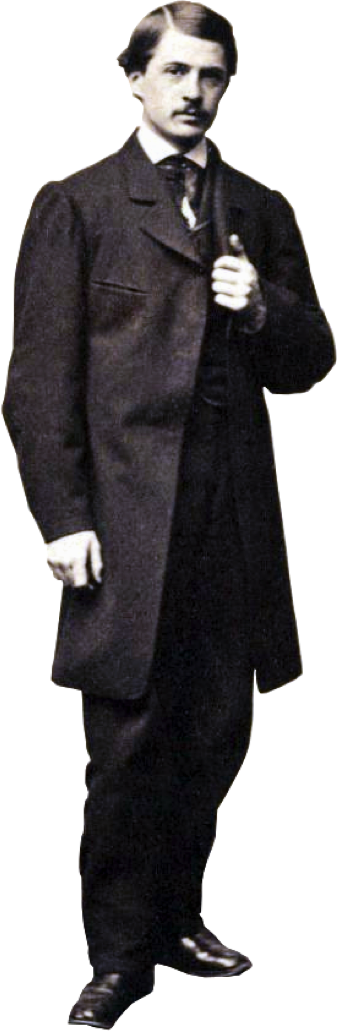
\includegraphics[width=1.7cm]{../figures/photo_pierce.png}
      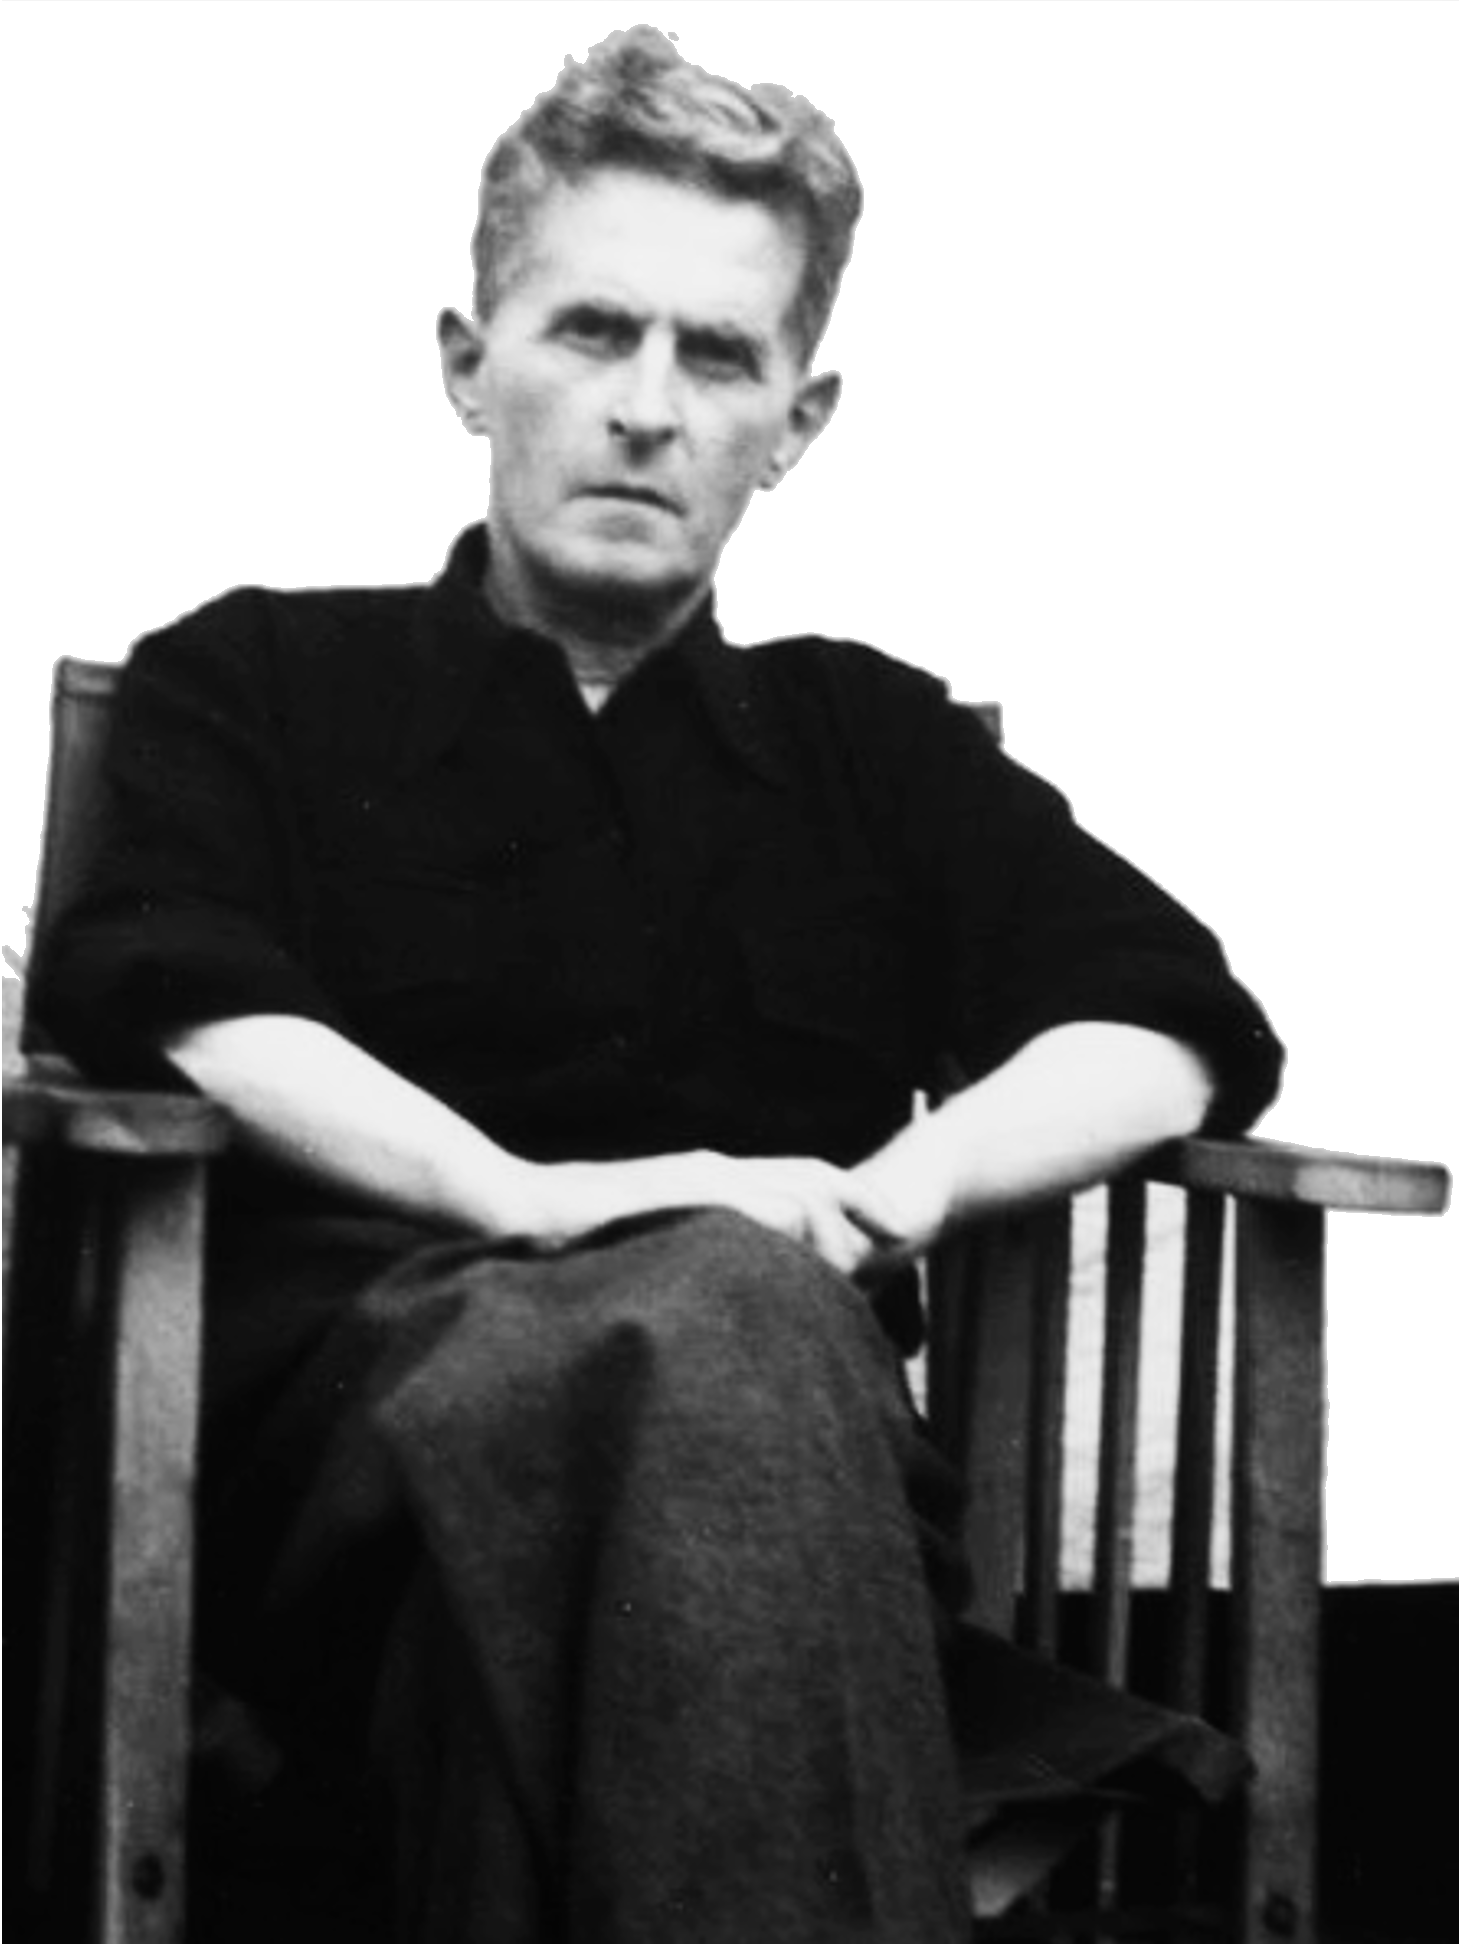
\includegraphics[width=2.6cm]{../figures/photo_wittgenstein.png}
    \end{column}
  \end{columns}
\end{frame}

\begin{frame}[fragile]{Common sources of syntax errors}
  \begin{itemize}
    \item Reading impairments (e.g., dyslexia, dysgraphia)
    \item Motor impairments (e.g., tremors, Parkinson's)
    \item Speech impediments (e.g., stuttering, apraxia, Tourette's)
    \item Visual impairments (e.g., poor eyesight, blindness)
    \item Language barriers (e.g., foreign and non-native speakers)
    \item Inexperience (e.g., novice programmers)
    \item Distraction (e.g., multitasking, fatigue, stress)
    \item Time pressure (e.g., deadlines, interview coding)
    \item Inattention (e.g., typographic mistakes, boredom, apathy)
    \item Lack of feedback (e.g., no syntax highlighting or IDE)
  \end{itemize}
\end{frame}

\begin{frame}[fragile]{Syntax repair as a language game}

  \begin{itemize}
    \item Imagine a game between two players, \textit{Editor} and \textit{Author}.
    \item They both see the same grammar, $\mathcal{G}$ and invalid string $\err\sigma \notin \mathcal{L}(\mathcal{G})$.
    % Both players move simultaneously after a short period of deliberation. As soon as Player A repairs $\err\sigma$, Player B must move immediately.
    \item Author moves by selecting a single valid string, $\sigma \in \mathcal{L}(\mathcal{G})$.
    \item Editor moves continuously, sampling a list of $\tilde{\bm\sigma} \in \mathcal{P}(\mathcal{L}(\mathcal{G}))$.
    \item As soon as Author repairs $\err\sigma$, the turn immediately ends.
    \item Neither player sees the other's move(s) before making their own.
    \item If Editor anticipates Author's move, i.e., $\sigma \in \tilde{\bm\sigma}$, they both win.
    \item If Author surprises Editor with a valid move, i.e., $\sigma \notin \tilde{\bm\sigma}$, Author wins.
    \item We may consider a refinement where Editor wins in proportion to the time taken to anticipate Author's move.
  \end{itemize}

\end{frame}
\begin{frame}{From Error-Correcting Codes to Correcting Coding Errors}
  \begin{itemize}
    \item Error-correcting codes are a well-studied topic in information theory used to detect and correct errors in data transmission.
    \item Introduces parity bits to detect and correct transmission errors assuming a certain noise model (e.g., Hamming distance).
    \item Like ECCs, we also assume a certain noise model (Levenshtein distance) and error tolerance (n-lexical tokens).
    \item Instead of injecting parity bits, we use the grammar and mutual information between tokens to detect and correct errors.
    \item Unlike ECCs, we do not assume a unique solution, but a set of admissible solutions ranked by statistical likliehood.
    \end{itemize}
  \setlength{\epigraphwidth}{0.97\textwidth}
  \epigraph{``\textit{Damn it, if the machine can detect an error, why can't it\\\phantom{``}locate the position of the error and correct it?'}''}{Richard Hamming, 1915-1998}
\end{frame}

\begin{frame}[fragile]{Our Contribution}
  Helps novice programmers fix syntax errors in source code. We do so by solving the \textbf{Realtime Bounded Levenshtein Reachability Problem}:\vspace{10pt}

  Given a context-free language $\ell: \mathcal{L}(\mathcal{G})$ and an invalid string $\err{\sigma}: \Sigma^*$, find every syntactically admissible edit $\tilde{\sigma}$ satisfying $\{\tilde{\sigma} \in \ell \mid \Delta(\err{\sigma}, \ell) < r\}$, ranked by a probability metric $\Delta$, under hard realtime constraints.

  \begin{center}
    \resizebox{0.42\textwidth}{!}{
      \def\secondcirclepath{(1.15,0) coordinate (e) circle (2cm)}
      \begin{tikzpicture}[
        dot/.style = {circle, inner sep=0pt, minimum size=1mm, fill,
        node contents={}}
      ]
        \def\firstcircle{(-2.1,0) coordinate (a) circle (2.4cm)}
        \def\firstcirclea{(-2.1,0) coordinate (b) circle (0.6cm)}
        \def\firstcircleb{(-2.1,0) coordinate (c) circle (1.2cm)}
        \def\firstcirclec{(-2.1,0) coordinate (d) circle (1.8cm)}
        \def\secondcircle{(1.2,0) coordinate (e) circle (1.5cm)}

        \begin{scope}
          \clip[decorate, decoration={snake, amplitude=0.6mm, segment length=5.01mm}] \secondcirclepath;
          \fill[black!15] \firstcircle;
        \end{scope}

        \draw \firstcircle node[dot,label=$\err{\sigma}$](z0);
        \draw [dashed] \firstcirclea;
        \draw [dashed] \firstcircleb;
        \draw [dashed] \firstcirclec;
        \draw[-stealth] (-2.1,0) -- (-1.5, 0) node[midway,below]{$d_1$};
        \draw[-stealth] (-1.5,0) -- (-0.9, 0) node[midway,below]{$d_2$};
        \draw[-stealth] (-0.9,0) -- (-0.3, 0) node[midway,below]{$d^*$};
        \draw[-stealth] (-0.3,0) -- (0.3, 0) node[midway,above]{$\tilde{\sigma}$};
        \draw[-stealth] (-0.3,0) -- (0.3, 0) node[midway,below]{$d^+$};

        \draw[decorate, decoration={snake, amplitude=0.6mm, segment length=5.01mm}] \secondcirclepath;
        \node [above] at (current bounding box.north -| a) {$\mathcal{L}\bigl(G(\err\sigma, d^*)\bigr)$};
        \node [above,yshift=2.1cm] at (e) {$\mathcal{L}(\mathcal{G}')$};
      \end{tikzpicture}
    }
    \scalebox{7}{\large$^+$\Huge\fontspec{Arial Unicode MS}^^^^231b}
  \end{center}

  \textbf{Natural language:}
  \textit{Rapidly finds syntactically valid edits within a small neighborhood, ranked by tokenwise similarity and statistical likliehood.}
\end{frame}

\begin{frame}[fragile]{Bounded Levenshtein Reachability}
  Syntax repair can be treated as a language intersection problem between a context-free language (CFL) and a regular language.

  \begin{definition}[Bounded Levenshtein-CFL reachability]
    Given a CFL $\ell$ and an invalid string $\err{\sigma}: \ell^\complement$, the BCFLR problem is to find every valid string reachable within $d$ edits of $\err{\sigma}$, i.e., we seek $L(\err\sigma, d) \cap \ell$ where $L(\err\sigma, d) \coloneqq \{\sigma \mid \Delta(\err{\sigma}, \sigma) \leq d\}$ and $\Delta$ is the Levenshtein metric.
  \end{definition}

  To solve this problem, we will first pose a simpler problem that only considers localized edits, then turn our attention back to BCFLR.

  \begin{definition}[Porous completion]
    Let $\underline\Sigma \coloneqq \Sigma \cup \{\_\}$, where $\_$ denotes a hole. We denote $\sqsubseteq: \Sigma^n \times \underline\Sigma^n$ as the relation $\{\langle\sigma', \sigma\rangle \mid \sigma_i \in \Sigma \implies \sigma_i' = \sigma_i\}$ and the set of all inhabitants $\{\sigma' \mid \sigma' \sqsubseteq \sigma\}$ as $\text{H}(\sigma)$. Given a \textit{porous string}, $\sigma: \underline\Sigma^*$ we seek all syntactically admissible inhabitants, i.e., $A(\sigma)\coloneqq\text{H}(\sigma)\cap\ell$.
  \end{definition}
\end{frame}

\begin{frame}[fragile]{Ranked repair under realtime constraints}
  $A(\sigma)$ is often a very large-cardinality set, so we want a procedure which prioritizes likely repairs first, without exhaustive enumeration. Specifically,
  \begin{definition}[Ranked repair]
    Given a finite language $\ell^\cap = L(\err\sigma, d) \cap \ell$ and a probabilistic language model $P_\theta: \Sigma^* \rightarrow [0, 1] \subset \mathbb{R}$, the ranked repair problem is to find the top-$k$ repairs by likelihood under the language model. That is,
    \begin{equation}
      R(\ell^\cap, P_\theta) \coloneqq \argmax_{\{\bm{\sigma} \mid \bm{\sigma} \subseteq \ell^\cap, |\bm{\sigma}| \leq k\}} \sum_{\sigma \in \bm{\sigma}}\text{P}(\sigma\mid\err\sigma, \theta)
    \end{equation}
    % On average, across all $G, \sigma$ $\hat{R}$ should approximate $R$.
    We want a procedure $\hat{R}$, minimizing $\mathbb{E}_{G, \sigma}\big[D_{\text{KL}}(\hat{R} \parallel R)\big]$ and total latency.
  \end{definition}
\end{frame}

\begin{frame}[fragile]{An Simple Reachability Proof}
  \begin{lemma}
    For any nonempty language $\ell: \mathcal{L}(\mathcal{G})$ and invalid string $\err{\sigma}: \Sigma^n$, there exists an $(\tilde{\sigma}, m)$ such that $\tilde{\sigma} \in \ell\cap\Sigma^m$ and $0 < \Delta(\err{\sigma}, \ell) \leq \max(m, n) < \infty$, where $\Delta$ denotes the Levenshtein edit distance.\\
  \end{lemma}

  \begin{proof}
  Since $\ell$ is nonempty, it must have at least one inhabitant $\sigma \in \ell$. Let $\tilde{\sigma}$ be the smallest such member. Since $\tilde{\sigma}$ is a valid sentence in $\ell$, by definition it must be that $|\tilde{\sigma}|<\infty$. Let $m:=|\tilde{\sigma}|$. Since we know $\err{\sigma} \notin \ell$, it follows that $0 < \Delta(\err{\sigma}, \ell)$. Let us consider two cases, either $\tilde{\sigma} = \varepsilon$, or $0 < |\tilde{\sigma}|$:

  \begin{itemize}
    \item If $\tilde{\sigma} = \varepsilon$, then $\Delta(\err{\sigma}, \tilde{\sigma}) = n$ by full erasure of $\err{\sigma}$, or
    \item If $0 < m$, then $\Delta(\err{\sigma}, \tilde{\sigma}) \leq \max(m, n)$ by overwriting.
  \end{itemize}

  In either case, it follows $\Delta(\err{\sigma}, \ell) \leq \max(m, n)$ and $\ell$ is always reachable via a finite nonempty set of Levenshtein edits, i.e., $0 < \Delta(\err{\sigma}, \ell) < \infty$.
    \end{proof}
\end{frame}

\begin{frame}[fragile]{From CFL Reachability to Real World Program Repair}
  To fix real code, we needed to overcome a variety of interesting challenges:\vspace{10pt}

  \begin{itemize}
    \item \textbf{Syntax mismatch}: The syntax of real-world programming languages does not exactly correspond to the theory of formal languages.
    \item \textbf{Source code $\approx$ PL}: Most of the time, source code in the wild is incomplete or only loosely approximates a programming language.
    \item \textbf{Responsiveness}: The usefulness of synthetic repairs is inversely proportional to the amount of time required to generate them.
    \item \textbf{Edit generation}: How do we generate edits that are (1) syntactically admissible (2) statistically plausible and (3) semantically meaningful?
    \item \textbf{Evaluation}: Big code and version control is too coarse-grained, contains irrelevant edits, not representative of small errors/fixes.
  \end{itemize}
\end{frame}

\begin{frame}[fragile]{High-level architecture overview}
  \begin{center}
    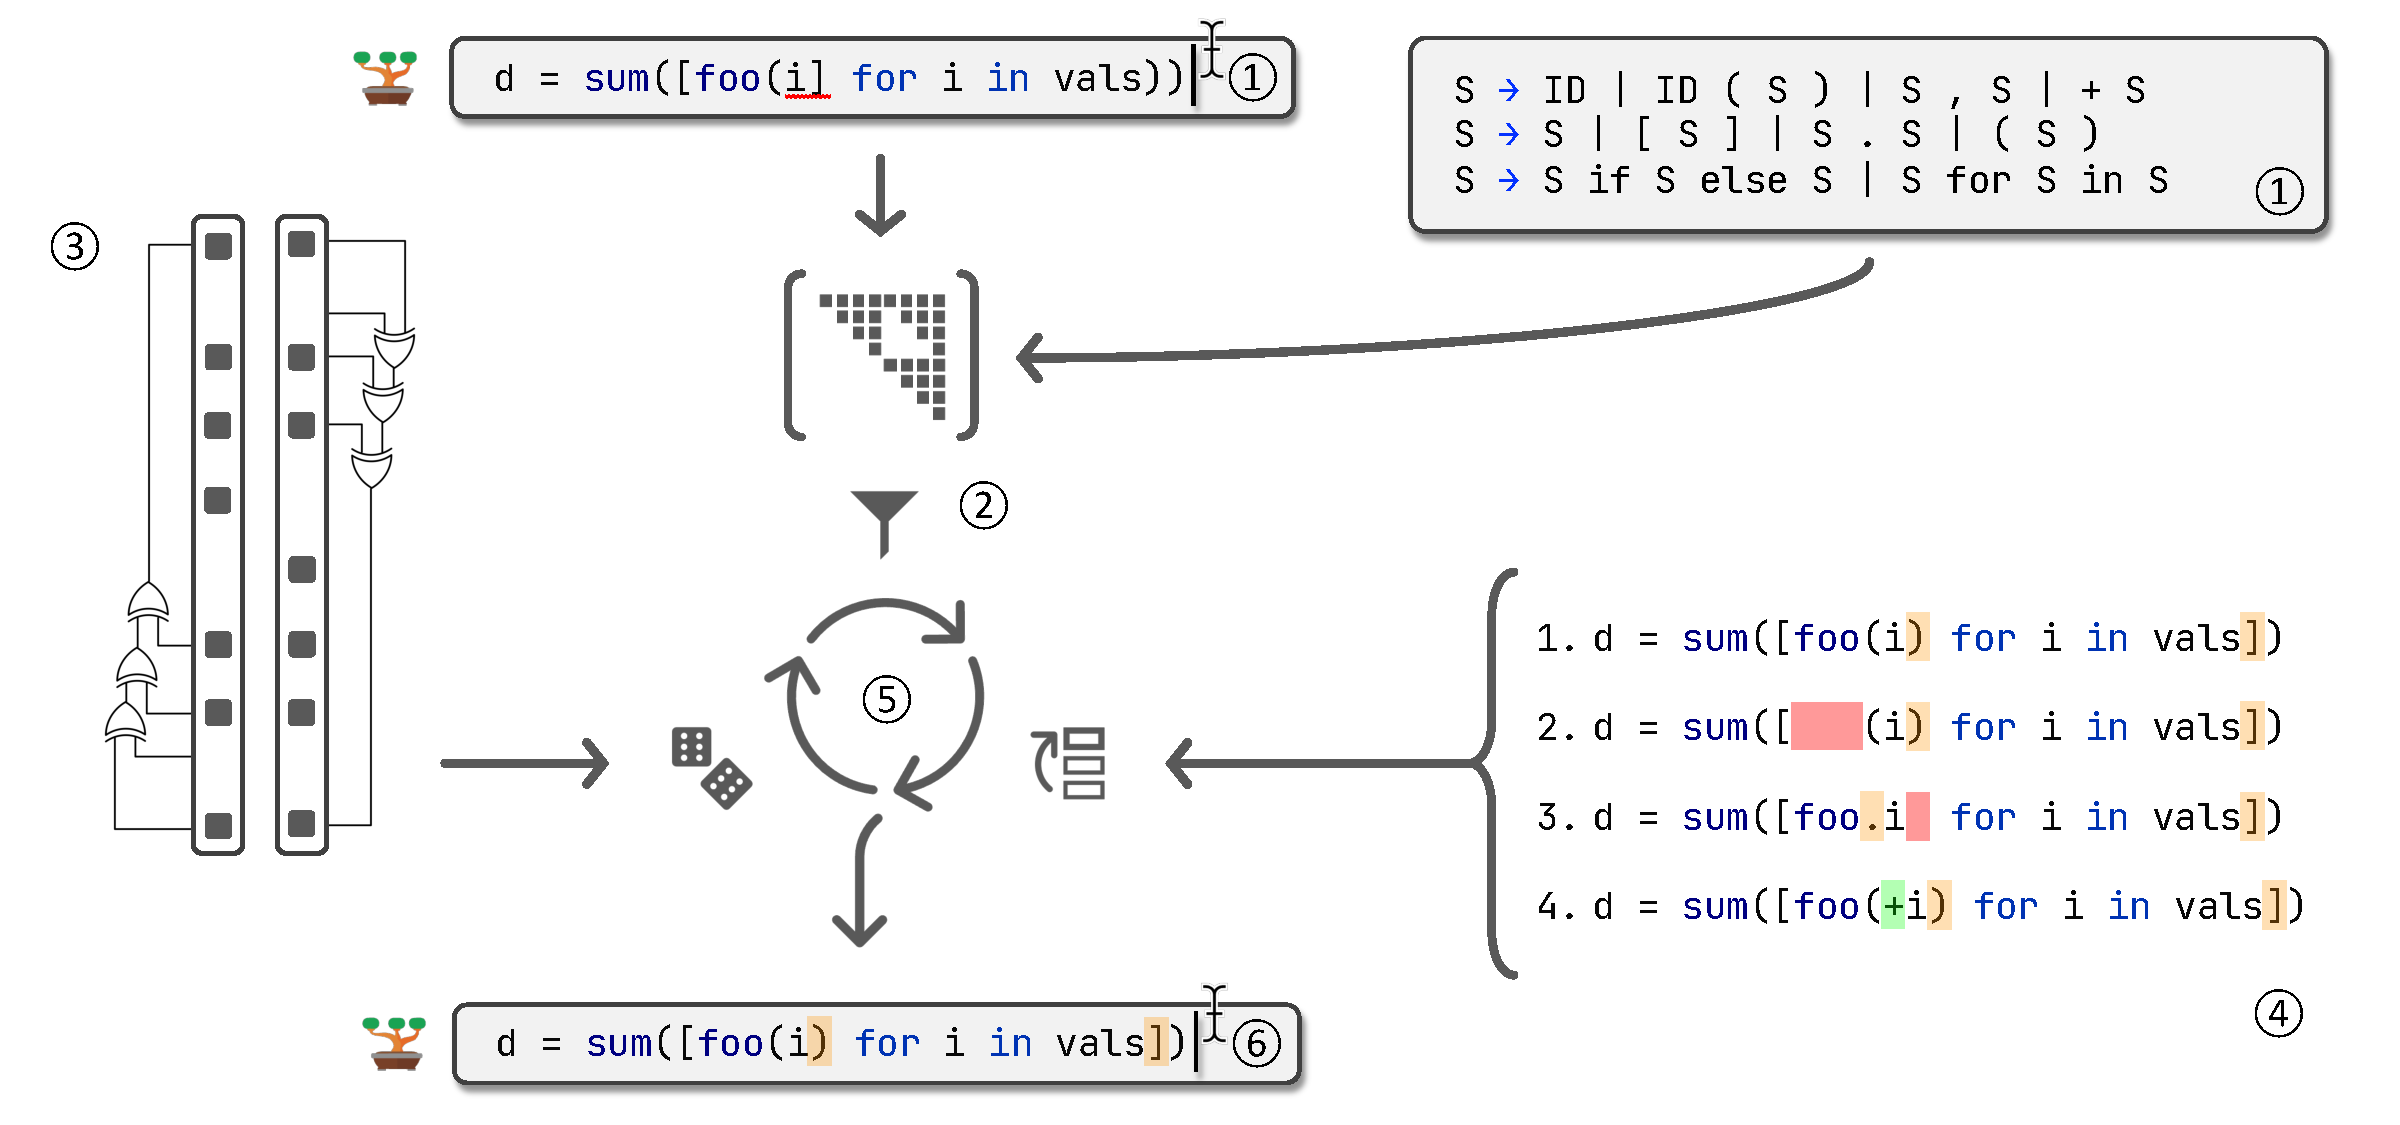
\includegraphics[width=0.9\linewidth]{../figures/architecture_overview.pdf}
  \end{center}
  \vspace{-10pt}
  \begin{footnotesize}
    Our framework consists of three components, (2) a solver, (4) ranker and (3) sampler. Given an invalid string and grammar (1), we first compile them into a multilinear system of equations which can be solved directly, yielding a set of repairs that are ranked using a suitable scoring function (4). Optionally, we may introduce stochastic edits to the string using the Levenshtein ball sampler (3) and extract the solutions incrementally (5).
  \end{footnotesize}
\end{frame}

\begin{frame}[fragile]{Uniform sampling benchmark on natural syntax errors}
  \begin{figure}[H]
    \resizebox{.3\textwidth}{!}{% This file was created with tikzplotlib v0.10.1.
\begin{tikzpicture}

\definecolor{darkgray176}{RGB}{176,176,176}
\definecolor{darkviolet1270255}{RGB}{127,0,255}
\definecolor{deepskyblue3176236}{RGB}{3,176,236}
\definecolor{dodgerblue45123246}{RGB}{45,123,246}
\definecolor{lightgray204}{RGB}{204,204,204}
\definecolor{royalblue8762253}{RGB}{87,62,253}

\begin{axis}[
legend cell align={left},
legend style={fill opacity=0.8, draw opacity=1, text opacity=1, draw=lightgray204, legend columns=-1, legend pos=north west},
tick align=outside,
tick pos=left,
title={$\Delta\in[1,3]$ Repair Precision},
x grid style={darkgray176},
xlabel={Seconds},
xmin=-0.4925, xmax=6.4925,
xtick style={color=black},
xtick={0,1,2,3,4,5,6},
xticklabels={20,60,100,140,180,220,260},
y grid style={darkgray176},
ylabel={Precision@k},
ymin=0, ymax=0.6741,
ytick style={color=black}
]
\addlegendimage{empty legend}
\addlegendentry{P@}
\draw[draw=none,fill=darkviolet1270255] (axis cs:-0.175,0) rectangle (axis cs:0.175,0.133);
\addlegendimage{ybar,ybar legend,draw=none,fill=darkviolet1270255}
\addlegendentry{All}

\draw[draw=none,fill=darkviolet1270255] (axis cs:0.825,0) rectangle (axis cs:1.175,0.272);
\draw[draw=none,fill=darkviolet1270255] (axis cs:1.825,0) rectangle (axis cs:2.175,0.382);
\draw[draw=none,fill=darkviolet1270255] (axis cs:2.825,0) rectangle (axis cs:3.175,0.474);
\draw[draw=none,fill=darkviolet1270255] (axis cs:3.825,0) rectangle (axis cs:4.175,0.543);
\draw[draw=none,fill=darkviolet1270255] (axis cs:4.825,0) rectangle (axis cs:5.175,0.618);
\draw[draw=none,fill=darkviolet1270255] (axis cs:5.825,0) rectangle (axis cs:6.175,0.642);
\draw[draw=none,fill=royalblue8762253] (axis cs:-0.175,0) rectangle (axis cs:0.175,0.133);
\addlegendimage{ybar,ybar legend,draw=none,fill=royalblue8762253}
\addlegendentry{10}

\draw[draw=none,fill=royalblue8762253] (axis cs:0.825,0) rectangle (axis cs:1.175,0.266);
\draw[draw=none,fill=royalblue8762253] (axis cs:1.825,0) rectangle (axis cs:2.175,0.353);
\draw[draw=none,fill=royalblue8762253] (axis cs:2.825,0) rectangle (axis cs:3.175,0.445);
\draw[draw=none,fill=royalblue8762253] (axis cs:3.825,0) rectangle (axis cs:4.175,0.509);
\draw[draw=none,fill=royalblue8762253] (axis cs:4.825,0) rectangle (axis cs:5.175,0.566);
\draw[draw=none,fill=royalblue8762253] (axis cs:5.825,0) rectangle (axis cs:6.175,0.572);
\draw[draw=none,fill=dodgerblue45123246] (axis cs:-0.175,0) rectangle (axis cs:0.175,0.133);
\addlegendimage{ybar,ybar legend,draw=none,fill=dodgerblue45123246}
\addlegendentry{5}

\draw[draw=none,fill=dodgerblue45123246] (axis cs:0.825,0) rectangle (axis cs:1.175,0.249);
\draw[draw=none,fill=dodgerblue45123246] (axis cs:1.825,0) rectangle (axis cs:2.175,0.335);
\draw[draw=none,fill=dodgerblue45123246] (axis cs:2.825,0) rectangle (axis cs:3.175,0.405);
\draw[draw=none,fill=dodgerblue45123246] (axis cs:3.825,0) rectangle (axis cs:4.175,0.445);
\draw[draw=none,fill=dodgerblue45123246] (axis cs:4.825,0) rectangle (axis cs:5.175,0.468);
\draw[draw=none,fill=dodgerblue45123246] (axis cs:5.825,0) rectangle (axis cs:6.175,0.474);
\draw[draw=none,fill=deepskyblue3176236] (axis cs:-0.175,0) rectangle (axis cs:0.175,0.098);
\addlegendimage{ybar,ybar legend,draw=none,fill=deepskyblue3176236}
\addlegendentry{1}

\draw[draw=none,fill=deepskyblue3176236] (axis cs:0.825,0) rectangle (axis cs:1.175,0.162);
\draw[draw=none,fill=deepskyblue3176236] (axis cs:1.825,0) rectangle (axis cs:2.175,0.202);
\draw[draw=none,fill=deepskyblue3176236] (axis cs:2.825,0) rectangle (axis cs:3.175,0.243);
\draw[draw=none,fill=deepskyblue3176236] (axis cs:3.825,0) rectangle (axis cs:4.175,0.272);
\draw[draw=none,fill=deepskyblue3176236] (axis cs:4.825,0) rectangle (axis cs:5.175,0.295);
\draw[draw=none,fill=deepskyblue3176236] (axis cs:5.825,0) rectangle (axis cs:6.175,0.306);
\end{axis}

\end{tikzpicture}
}
    \resizebox{.3\textwidth}{!}{% This file was created with tikzplotlib v0.10.1.
\begin{tikzpicture}

\definecolor{darkgray176}{RGB}{176,176,176}
\definecolor{darkviolet1270255}{RGB}{127,0,255}
\definecolor{deepskyblue3176236}{RGB}{3,176,236}
\definecolor{dodgerblue45123246}{RGB}{45,123,246}
\definecolor{lightgray204}{RGB}{204,204,204}
\definecolor{royalblue8762253}{RGB}{87,62,253}

\begin{axis}[
legend cell align={left},
legend style={fill opacity=0.8, draw opacity=1, text opacity=1, draw=lightgray204, legend columns=-1, legend pos=north west},
tick align=outside,
tick pos=left,
title={$\Delta=1$ Repair Precision},
x grid style={darkgray176},
xlabel={Seconds},
xmin=-0.4925, xmax=6.4925,
xtick style={color=black},
xtick={0,1,2,3,4,5,6},
xticklabels={20,60,100,140,180,220,260},
y grid style={darkgray176},
ylabel={\phantom{Precision@k}},
ymin=0, ymax=0.77595,
ytick style={color=black}
]
\addlegendimage{empty legend}
\addlegendentry{P@}
\draw[draw=none,fill=darkviolet1270255] (axis cs:-0.175,0) rectangle (axis cs:0.175,0.145);
\addlegendimage{ybar,ybar legend,draw=none,fill=darkviolet1270255}
\addlegendentry{All}

\draw[draw=none,fill=darkviolet1270255] (axis cs:0.825,0) rectangle (axis cs:1.175,0.304);
\draw[draw=none,fill=darkviolet1270255] (axis cs:1.825,0) rectangle (axis cs:2.175,0.42);
\draw[draw=none,fill=darkviolet1270255] (axis cs:2.825,0) rectangle (axis cs:3.175,0.507);
\draw[draw=none,fill=darkviolet1270255] (axis cs:3.825,0) rectangle (axis cs:4.175,0.594);
\draw[draw=none,fill=darkviolet1270255] (axis cs:4.825,0) rectangle (axis cs:5.175,0.71);
\draw[draw=none,fill=darkviolet1270255] (axis cs:5.825,0) rectangle (axis cs:6.175,0.739);
\draw[draw=none,fill=royalblue8762253] (axis cs:-0.175,0) rectangle (axis cs:0.175,0.145);
\addlegendimage{ybar,ybar legend,draw=none,fill=royalblue8762253}
\addlegendentry{10}

\draw[draw=none,fill=royalblue8762253] (axis cs:0.825,0) rectangle (axis cs:1.175,0.304);
\draw[draw=none,fill=royalblue8762253] (axis cs:1.825,0) rectangle (axis cs:2.175,0.42);
\draw[draw=none,fill=royalblue8762253] (axis cs:2.825,0) rectangle (axis cs:3.175,0.507);
\draw[draw=none,fill=royalblue8762253] (axis cs:3.825,0) rectangle (axis cs:4.175,0.594);
\draw[draw=none,fill=royalblue8762253] (axis cs:4.825,0) rectangle (axis cs:5.175,0.703);
\draw[draw=none,fill=royalblue8762253] (axis cs:5.825,0) rectangle (axis cs:6.175,0.732);
\draw[draw=none,fill=dodgerblue45123246] (axis cs:-0.175,0) rectangle (axis cs:0.175,0.145);
\addlegendimage{ybar,ybar legend,draw=none,fill=dodgerblue45123246}
\addlegendentry{5}

\draw[draw=none,fill=dodgerblue45123246] (axis cs:0.825,0) rectangle (axis cs:1.175,0.304);
\draw[draw=none,fill=dodgerblue45123246] (axis cs:1.825,0) rectangle (axis cs:2.175,0.42);
\draw[draw=none,fill=dodgerblue45123246] (axis cs:2.825,0) rectangle (axis cs:3.175,0.493);
\draw[draw=none,fill=dodgerblue45123246] (axis cs:3.825,0) rectangle (axis cs:4.175,0.565);
\draw[draw=none,fill=dodgerblue45123246] (axis cs:4.825,0) rectangle (axis cs:5.175,0.638);
\draw[draw=none,fill=dodgerblue45123246] (axis cs:5.825,0) rectangle (axis cs:6.175,0.667);
\draw[draw=none,fill=deepskyblue3176236] (axis cs:-0.175,0) rectangle (axis cs:0.175,0.116);
\addlegendimage{ybar,ybar legend,draw=none,fill=deepskyblue3176236}
\addlegendentry{1}

\draw[draw=none,fill=deepskyblue3176236] (axis cs:0.825,0) rectangle (axis cs:1.175,0.203);
\draw[draw=none,fill=deepskyblue3176236] (axis cs:1.825,0) rectangle (axis cs:2.175,0.268);
\draw[draw=none,fill=deepskyblue3176236] (axis cs:2.825,0) rectangle (axis cs:3.175,0.312);
\draw[draw=none,fill=deepskyblue3176236] (axis cs:3.825,0) rectangle (axis cs:4.175,0.355);
\draw[draw=none,fill=deepskyblue3176236] (axis cs:4.825,0) rectangle (axis cs:5.175,0.428);
\draw[draw=none,fill=deepskyblue3176236] (axis cs:5.825,0) rectangle (axis cs:6.175,0.442);
\end{axis}

\end{tikzpicture}
}
    \resizebox{.3\textwidth}{!}{% This file was created with tikzplotlib v0.10.1.
\begin{tikzpicture}

\definecolor{darkgray176}{RGB}{176,176,176}
\definecolor{darkviolet1270255}{RGB}{127,0,255}
\definecolor{deepskyblue3176236}{RGB}{3,176,236}
\definecolor{dodgerblue45123246}{RGB}{45,123,246}
\definecolor{lightgray204}{RGB}{204,204,204}
\definecolor{royalblue8762253}{RGB}{87,62,253}

\begin{axis}[
legend cell align={left},
legend style={fill opacity=0.8, draw opacity=1, text opacity=1, draw=lightgray204, legend columns=-1, legend pos=north west},
tick align=outside,
tick pos=left,
title={$\Delta=2$ Repair Precision},
x grid style={darkgray176},
xlabel={Seconds},
xmin=-0.4925, xmax=6.4925,
xtick style={color=black},
xtick={0,1,2,3,4,5,6},
xticklabels={20,60,100,140,180,220,260},
y grid style={darkgray176},
ylabel={\phantom{Precision@k}},
ymin=0, ymax=0.40635,
ytick style={color=black}
]
\addlegendimage{empty legend}
\addlegendentry{P@}
\draw[draw=none,fill=darkviolet1270255] (axis cs:-0.175,0) rectangle (axis cs:0.175,0.048);
\addlegendimage{ybar,ybar legend,draw=none,fill=darkviolet1270255}
\addlegendentry{All}

\draw[draw=none,fill=darkviolet1270255] (axis cs:0.825,0) rectangle (axis cs:1.175,0.081);
\draw[draw=none,fill=darkviolet1270255] (axis cs:1.825,0) rectangle (axis cs:2.175,0.177);
\draw[draw=none,fill=darkviolet1270255] (axis cs:2.825,0) rectangle (axis cs:3.175,0.274);
\draw[draw=none,fill=darkviolet1270255] (axis cs:3.825,0) rectangle (axis cs:4.175,0.306);
\draw[draw=none,fill=darkviolet1270255] (axis cs:4.825,0) rectangle (axis cs:5.175,0.355);
\draw[draw=none,fill=darkviolet1270255] (axis cs:5.825,0) rectangle (axis cs:6.175,0.387);
\draw[draw=none,fill=royalblue8762253] (axis cs:-0.175,0) rectangle (axis cs:0.175,0.048);
\addlegendimage{ybar,ybar legend,draw=none,fill=royalblue8762253}
\addlegendentry{10}

\draw[draw=none,fill=royalblue8762253] (axis cs:0.825,0) rectangle (axis cs:1.175,0.081);
\draw[draw=none,fill=royalblue8762253] (axis cs:1.825,0) rectangle (axis cs:2.175,0.113);
\draw[draw=none,fill=royalblue8762253] (axis cs:2.825,0) rectangle (axis cs:3.175,0.21);
\draw[draw=none,fill=royalblue8762253] (axis cs:3.825,0) rectangle (axis cs:4.175,0.226);
\draw[draw=none,fill=royalblue8762253] (axis cs:4.825,0) rectangle (axis cs:5.175,0.258);
\draw[draw=none,fill=royalblue8762253] (axis cs:5.825,0) rectangle (axis cs:6.175,0.242);
\draw[draw=none,fill=dodgerblue45123246] (axis cs:-0.175,0) rectangle (axis cs:0.175,0.048);
\addlegendimage{ybar,ybar legend,draw=none,fill=dodgerblue45123246}
\addlegendentry{5}

\draw[draw=none,fill=dodgerblue45123246] (axis cs:0.825,0) rectangle (axis cs:1.175,0.032);
\draw[draw=none,fill=dodgerblue45123246] (axis cs:1.825,0) rectangle (axis cs:2.175,0.065);
\draw[draw=none,fill=dodgerblue45123246] (axis cs:2.825,0) rectangle (axis cs:3.175,0.129);
\draw[draw=none,fill=dodgerblue45123246] (axis cs:3.825,0) rectangle (axis cs:4.175,0.113);
\draw[draw=none,fill=dodgerblue45123246] (axis cs:4.825,0) rectangle (axis cs:5.175,0.129);
\draw[draw=none,fill=dodgerblue45123246] (axis cs:5.825,0) rectangle (axis cs:6.175,0.113);
\draw[draw=none,fill=deepskyblue3176236] (axis cs:-0.175,0) rectangle (axis cs:0.175,0.016);
\addlegendimage{ybar,ybar legend,draw=none,fill=deepskyblue3176236}
\addlegendentry{1}

\draw[draw=none,fill=deepskyblue3176236] (axis cs:0.825,0) rectangle (axis cs:1.175,0);
\draw[draw=none,fill=deepskyblue3176236] (axis cs:1.825,0) rectangle (axis cs:2.175,0.016);
\draw[draw=none,fill=deepskyblue3176236] (axis cs:2.825,0) rectangle (axis cs:3.175,0.065);
\draw[draw=none,fill=deepskyblue3176236] (axis cs:3.825,0) rectangle (axis cs:4.175,0.048);
\draw[draw=none,fill=deepskyblue3176236] (axis cs:4.825,0) rectangle (axis cs:5.175,0.032);
\draw[draw=none,fill=deepskyblue3176236] (axis cs:5.825,0) rectangle (axis cs:6.175,0.032);
\end{axis}

\end{tikzpicture}
}
%\resizebox{.3\textwidth}{!}{% This file was created with tikzplotlib v0.10.1.
\begin{tikzpicture}

\definecolor{darkgray176}{RGB}{176,176,176}
\definecolor{darkviolet1270255}{RGB}{127,0,255}
\definecolor{deepskyblue3176236}{RGB}{3,176,236}
\definecolor{dodgerblue45123246}{RGB}{45,123,246}
\definecolor{lightgray204}{RGB}{204,204,204}
\definecolor{royalblue8762253}{RGB}{87,62,253}

\begin{axis}[
legend cell align={left},
legend style={fill opacity=0.8, draw opacity=1, text opacity=1, draw=lightgray204, legend columns=-1, legend pos=north west},
tick align=outside,
tick pos=left,
title={$\Delta=1$ Repair Precision},
x grid style={darkgray176},
xlabel={Seconds},
xmin=-0.4925, xmax=6.4925,
xtick style={color=black},
xtick={0,1,2,3,4,5,6},
xticklabels={20,60,100,140,180,220,260},
y grid style={darkgray176},
ylabel={\phantom{Precision@k}},
ymin=0, ymax=0.77595,
ytick style={color=black}
]
\addlegendimage{empty legend}
\addlegendentry{P@}
\draw[draw=none,fill=darkviolet1270255] (axis cs:-0.175,0) rectangle (axis cs:0.175,0.145);
\addlegendimage{ybar,ybar legend,draw=none,fill=darkviolet1270255}
\addlegendentry{All}

\draw[draw=none,fill=darkviolet1270255] (axis cs:0.825,0) rectangle (axis cs:1.175,0.304);
\draw[draw=none,fill=darkviolet1270255] (axis cs:1.825,0) rectangle (axis cs:2.175,0.42);
\draw[draw=none,fill=darkviolet1270255] (axis cs:2.825,0) rectangle (axis cs:3.175,0.507);
\draw[draw=none,fill=darkviolet1270255] (axis cs:3.825,0) rectangle (axis cs:4.175,0.594);
\draw[draw=none,fill=darkviolet1270255] (axis cs:4.825,0) rectangle (axis cs:5.175,0.71);
\draw[draw=none,fill=darkviolet1270255] (axis cs:5.825,0) rectangle (axis cs:6.175,0.739);
\draw[draw=none,fill=royalblue8762253] (axis cs:-0.175,0) rectangle (axis cs:0.175,0.145);
\addlegendimage{ybar,ybar legend,draw=none,fill=royalblue8762253}
\addlegendentry{10}

\draw[draw=none,fill=royalblue8762253] (axis cs:0.825,0) rectangle (axis cs:1.175,0.304);
\draw[draw=none,fill=royalblue8762253] (axis cs:1.825,0) rectangle (axis cs:2.175,0.42);
\draw[draw=none,fill=royalblue8762253] (axis cs:2.825,0) rectangle (axis cs:3.175,0.507);
\draw[draw=none,fill=royalblue8762253] (axis cs:3.825,0) rectangle (axis cs:4.175,0.594);
\draw[draw=none,fill=royalblue8762253] (axis cs:4.825,0) rectangle (axis cs:5.175,0.703);
\draw[draw=none,fill=royalblue8762253] (axis cs:5.825,0) rectangle (axis cs:6.175,0.732);
\draw[draw=none,fill=dodgerblue45123246] (axis cs:-0.175,0) rectangle (axis cs:0.175,0.145);
\addlegendimage{ybar,ybar legend,draw=none,fill=dodgerblue45123246}
\addlegendentry{5}

\draw[draw=none,fill=dodgerblue45123246] (axis cs:0.825,0) rectangle (axis cs:1.175,0.304);
\draw[draw=none,fill=dodgerblue45123246] (axis cs:1.825,0) rectangle (axis cs:2.175,0.42);
\draw[draw=none,fill=dodgerblue45123246] (axis cs:2.825,0) rectangle (axis cs:3.175,0.493);
\draw[draw=none,fill=dodgerblue45123246] (axis cs:3.825,0) rectangle (axis cs:4.175,0.565);
\draw[draw=none,fill=dodgerblue45123246] (axis cs:4.825,0) rectangle (axis cs:5.175,0.638);
\draw[draw=none,fill=dodgerblue45123246] (axis cs:5.825,0) rectangle (axis cs:6.175,0.667);
\draw[draw=none,fill=deepskyblue3176236] (axis cs:-0.175,0) rectangle (axis cs:0.175,0.116);
\addlegendimage{ybar,ybar legend,draw=none,fill=deepskyblue3176236}
\addlegendentry{1}

\draw[draw=none,fill=deepskyblue3176236] (axis cs:0.825,0) rectangle (axis cs:1.175,0.203);
\draw[draw=none,fill=deepskyblue3176236] (axis cs:1.825,0) rectangle (axis cs:2.175,0.268);
\draw[draw=none,fill=deepskyblue3176236] (axis cs:2.825,0) rectangle (axis cs:3.175,0.312);
\draw[draw=none,fill=deepskyblue3176236] (axis cs:3.825,0) rectangle (axis cs:4.175,0.355);
\draw[draw=none,fill=deepskyblue3176236] (axis cs:4.825,0) rectangle (axis cs:5.175,0.428);
\draw[draw=none,fill=deepskyblue3176236] (axis cs:5.825,0) rectangle (axis cs:6.175,0.442);
\end{axis}

\end{tikzpicture}
}
%\resizebox{.307\textwidth}{!}{% This file was created with tikzplotlib v0.10.1.
\begin{tikzpicture}

\definecolor{darkgray176}{RGB}{176,176,176}
\definecolor{darkviolet1270255}{RGB}{127,0,255}
\definecolor{deepskyblue3176236}{RGB}{3,176,236}
\definecolor{dodgerblue45123246}{RGB}{45,123,246}
\definecolor{lightgray204}{RGB}{204,204,204}
\definecolor{royalblue8762253}{RGB}{87,62,253}

\begin{axis}[
legend cell align={left},
legend style={fill opacity=0.8, draw opacity=1, text opacity=1, draw=lightgray204, legend columns=-1, legend pos=north west},
tick align=outside,
tick pos=left,
title={$\Delta=2$ Repair Precision},
x grid style={darkgray176},
xlabel={Seconds},
xmin=-0.4925, xmax=6.4925,
xtick style={color=black},
xtick={0,1,2,3,4,5,6},
xticklabels={20,60,100,140,180,220,260},
y grid style={darkgray176},
ylabel={\phantom{Precision@k}},
ymin=0, ymax=0.40635,
ytick style={color=black}
]
\addlegendimage{empty legend}
\addlegendentry{P@}
\draw[draw=none,fill=darkviolet1270255] (axis cs:-0.175,0) rectangle (axis cs:0.175,0.048);
\addlegendimage{ybar,ybar legend,draw=none,fill=darkviolet1270255}
\addlegendentry{All}

\draw[draw=none,fill=darkviolet1270255] (axis cs:0.825,0) rectangle (axis cs:1.175,0.081);
\draw[draw=none,fill=darkviolet1270255] (axis cs:1.825,0) rectangle (axis cs:2.175,0.177);
\draw[draw=none,fill=darkviolet1270255] (axis cs:2.825,0) rectangle (axis cs:3.175,0.274);
\draw[draw=none,fill=darkviolet1270255] (axis cs:3.825,0) rectangle (axis cs:4.175,0.306);
\draw[draw=none,fill=darkviolet1270255] (axis cs:4.825,0) rectangle (axis cs:5.175,0.355);
\draw[draw=none,fill=darkviolet1270255] (axis cs:5.825,0) rectangle (axis cs:6.175,0.387);
\draw[draw=none,fill=royalblue8762253] (axis cs:-0.175,0) rectangle (axis cs:0.175,0.048);
\addlegendimage{ybar,ybar legend,draw=none,fill=royalblue8762253}
\addlegendentry{10}

\draw[draw=none,fill=royalblue8762253] (axis cs:0.825,0) rectangle (axis cs:1.175,0.081);
\draw[draw=none,fill=royalblue8762253] (axis cs:1.825,0) rectangle (axis cs:2.175,0.113);
\draw[draw=none,fill=royalblue8762253] (axis cs:2.825,0) rectangle (axis cs:3.175,0.21);
\draw[draw=none,fill=royalblue8762253] (axis cs:3.825,0) rectangle (axis cs:4.175,0.226);
\draw[draw=none,fill=royalblue8762253] (axis cs:4.825,0) rectangle (axis cs:5.175,0.258);
\draw[draw=none,fill=royalblue8762253] (axis cs:5.825,0) rectangle (axis cs:6.175,0.242);
\draw[draw=none,fill=dodgerblue45123246] (axis cs:-0.175,0) rectangle (axis cs:0.175,0.048);
\addlegendimage{ybar,ybar legend,draw=none,fill=dodgerblue45123246}
\addlegendentry{5}

\draw[draw=none,fill=dodgerblue45123246] (axis cs:0.825,0) rectangle (axis cs:1.175,0.032);
\draw[draw=none,fill=dodgerblue45123246] (axis cs:1.825,0) rectangle (axis cs:2.175,0.065);
\draw[draw=none,fill=dodgerblue45123246] (axis cs:2.825,0) rectangle (axis cs:3.175,0.129);
\draw[draw=none,fill=dodgerblue45123246] (axis cs:3.825,0) rectangle (axis cs:4.175,0.113);
\draw[draw=none,fill=dodgerblue45123246] (axis cs:4.825,0) rectangle (axis cs:5.175,0.129);
\draw[draw=none,fill=dodgerblue45123246] (axis cs:5.825,0) rectangle (axis cs:6.175,0.113);
\draw[draw=none,fill=deepskyblue3176236] (axis cs:-0.175,0) rectangle (axis cs:0.175,0.016);
\addlegendimage{ybar,ybar legend,draw=none,fill=deepskyblue3176236}
\addlegendentry{1}

\draw[draw=none,fill=deepskyblue3176236] (axis cs:0.825,0) rectangle (axis cs:1.175,0);
\draw[draw=none,fill=deepskyblue3176236] (axis cs:1.825,0) rectangle (axis cs:2.175,0.016);
\draw[draw=none,fill=deepskyblue3176236] (axis cs:2.825,0) rectangle (axis cs:3.175,0.065);
\draw[draw=none,fill=deepskyblue3176236] (axis cs:3.825,0) rectangle (axis cs:4.175,0.048);
\draw[draw=none,fill=deepskyblue3176236] (axis cs:4.825,0) rectangle (axis cs:5.175,0.032);
\draw[draw=none,fill=deepskyblue3176236] (axis cs:5.825,0) rectangle (axis cs:6.175,0.032);
\end{axis}

\end{tikzpicture}
}
    \caption{Repairs discovered before the latency cutoff are reranked based on their tokenwise perplexity and compared for an exact lexical match with the human repair at or below rank k. We note that the uniform sampling procedure is not intended to be used in practice, but provides a baseline for the empirical density of the admissible set, and an upper bound on the latency required to attain a given precision.}\label{fig:human}
  \end{figure}
\end{frame}

\begin{frame}[fragile]{Adaptive sampling benchmark on natural syntax errors}
  \begin{figure}[H]
    \resizebox{.24\textwidth}{!}{% This file was created with tikzplotlib v0.10.1.
\begin{tikzpicture}

\definecolor{darkgray176}{RGB}{176,176,176}
\definecolor{darkviolet1270255}{RGB}{127,0,255}
\definecolor{deepskyblue3176236}{RGB}{3,176,236}
\definecolor{dodgerblue45123246}{RGB}{45,123,246}
\definecolor{lightgray204}{RGB}{204,204,204}
\definecolor{royalblue8762253}{RGB}{87,62,253}

\begin{axis}[
legend cell align={left},
legend style={fill opacity=0.8, draw opacity=1, text opacity=1, draw=lightgray204, legend columns=-1, legend pos=north west},
tick align=outside,
tick pos=left,
title={\(\displaystyle \Delta\in[1,3]\) Repair Precision},
x grid style={darkgray176},
xlabel={Seconds},
xmin=-0.5925, xmax=8.5925,
ymin=0.0, ymax=0.7,
xtick style={color=black},
xtick={0,1,2,3,4,5,6,7,8},
xticklabels={0.1,0.3,0.5,0.7,0.9,1.1,1.3,1.5,1.7},
y grid style={darkgray176},
ylabel={Precision@k},
ytick style={color=black},
width=0.5\textwidth,
height=0.48\textwidth,
]
\addlegendimage{empty legend}
\addlegendentry{P@}
\draw[draw=none,fill=darkviolet1270255] (axis cs:-0.175,0) rectangle (axis cs:0.175,0.245);
\addlegendimage{ybar,ybar legend,draw=none,fill=darkviolet1270255}
\addlegendentry{All}

\draw[draw=none,fill=darkviolet1270255] (axis cs:0.825,0) rectangle (axis cs:1.175,0.417);
\draw[draw=none,fill=darkviolet1270255] (axis cs:1.825,0) rectangle (axis cs:2.175,0.496);
\draw[draw=none,fill=darkviolet1270255] (axis cs:2.825,0) rectangle (axis cs:3.175,0.535);
\draw[draw=none,fill=darkviolet1270255] (axis cs:3.825,0) rectangle (axis cs:4.175,0.562);
\draw[draw=none,fill=darkviolet1270255] (axis cs:4.825,0) rectangle (axis cs:5.175,0.584);
\draw[draw=none,fill=darkviolet1270255] (axis cs:5.825,0) rectangle (axis cs:6.175,0.603);
\draw[draw=none,fill=darkviolet1270255] (axis cs:6.825,0) rectangle (axis cs:7.175,0.619);
\draw[draw=none,fill=darkviolet1270255] (axis cs:7.825,0) rectangle (axis cs:8.175,0.629);
\draw[draw=none,fill=royalblue8762253] (axis cs:-0.175,0) rectangle (axis cs:0.175,0.234);
\addlegendimage{ybar,ybar legend,draw=none,fill=royalblue8762253}
\addlegendentry{10}

\draw[draw=none,fill=royalblue8762253] (axis cs:0.825,0) rectangle (axis cs:1.175,0.387);
\draw[draw=none,fill=royalblue8762253] (axis cs:1.825,0) rectangle (axis cs:2.175,0.451);
\draw[draw=none,fill=royalblue8762253] (axis cs:2.825,0) rectangle (axis cs:3.175,0.481);
\draw[draw=none,fill=royalblue8762253] (axis cs:3.825,0) rectangle (axis cs:4.175,0.502);
\draw[draw=none,fill=royalblue8762253] (axis cs:4.825,0) rectangle (axis cs:5.175,0.517);
\draw[draw=none,fill=royalblue8762253] (axis cs:5.825,0) rectangle (axis cs:6.175,0.53);
\draw[draw=none,fill=royalblue8762253] (axis cs:6.825,0) rectangle (axis cs:7.175,0.54);
\draw[draw=none,fill=royalblue8762253] (axis cs:7.825,0) rectangle (axis cs:8.175,0.546);
\draw[draw=none,fill=dodgerblue45123246] (axis cs:-0.175,0) rectangle (axis cs:0.175,0.218);
\addlegendimage{ybar,ybar legend,draw=none,fill=dodgerblue45123246}
\addlegendentry{5}

\draw[draw=none,fill=dodgerblue45123246] (axis cs:0.825,0) rectangle (axis cs:1.175,0.353);
\draw[draw=none,fill=dodgerblue45123246] (axis cs:1.825,0) rectangle (axis cs:2.175,0.406);
\draw[draw=none,fill=dodgerblue45123246] (axis cs:2.825,0) rectangle (axis cs:3.175,0.43);
\draw[draw=none,fill=dodgerblue45123246] (axis cs:3.825,0) rectangle (axis cs:4.175,0.444);
\draw[draw=none,fill=dodgerblue45123246] (axis cs:4.825,0) rectangle (axis cs:5.175,0.455);
\draw[draw=none,fill=dodgerblue45123246] (axis cs:5.825,0) rectangle (axis cs:6.175,0.467);
\draw[draw=none,fill=dodgerblue45123246] (axis cs:6.825,0) rectangle (axis cs:7.175,0.474);
\draw[draw=none,fill=dodgerblue45123246] (axis cs:7.825,0) rectangle (axis cs:8.175,0.479);
\draw[draw=none,fill=deepskyblue3176236] (axis cs:-0.175,0) rectangle (axis cs:0.175,0.117);
\addlegendimage{ybar,ybar legend,draw=none,fill=deepskyblue3176236}
\addlegendentry{1}

\draw[draw=none,fill=deepskyblue3176236] (axis cs:0.825,0) rectangle (axis cs:1.175,0.187);
\draw[draw=none,fill=deepskyblue3176236] (axis cs:1.825,0) rectangle (axis cs:2.175,0.219);
\draw[draw=none,fill=deepskyblue3176236] (axis cs:2.825,0) rectangle (axis cs:3.175,0.233);
\draw[draw=none,fill=deepskyblue3176236] (axis cs:3.825,0) rectangle (axis cs:4.175,0.244);
\draw[draw=none,fill=deepskyblue3176236] (axis cs:4.825,0) rectangle (axis cs:5.175,0.25);
\draw[draw=none,fill=deepskyblue3176236] (axis cs:5.825,0) rectangle (axis cs:6.175,0.258);
\draw[draw=none,fill=deepskyblue3176236] (axis cs:6.825,0) rectangle (axis cs:7.175,0.262);
\draw[draw=none,fill=deepskyblue3176236] (axis cs:7.825,0) rectangle (axis cs:8.175,0.265);
\addplot [red, thick] coordinates {(-0.8925,0.35) (14.8925,0.35)};
\end{axis}

\end{tikzpicture}
}
    \resizebox{.25\textwidth}{!}{% This file was created with tikzplotlib v0.10.1.
\begin{tikzpicture}

\definecolor{darkgray176}{RGB}{176,176,176}
\definecolor{darkviolet1270255}{RGB}{127,0,255}
\definecolor{deepskyblue3176236}{RGB}{3,176,236}
\definecolor{dodgerblue45123246}{RGB}{45,123,246}
\definecolor{lightgray204}{RGB}{204,204,204}
\definecolor{royalblue8762253}{RGB}{87,62,253}

\begin{axis}[
legend cell align={left},
legend style={fill opacity=0.8, draw opacity=1, text opacity=1, draw=lightgray204, legend columns=-1, legend pos=north west},
tick align=outside,
tick pos=left,
title={$\Delta=1$ Repair Precision},
x grid style={darkgray176},
xlabel={Seconds},
xmin=-0.5925, xmax=8.5925,
xtick style={color=black},
xtick={0,1,2,3,4,5,6,7,8},
xticklabels={0.1,0.3,0.5,0.7,0.9,1.1,1.3,1.5,1.7},
y grid style={darkgray176},
ymin=0, ymax=1.0,
ytick style={color=black}
width=0.43\textwidth,
height=0.49\textwidth,
]
\addlegendimage{empty legend}
\addlegendentry{P@}
\draw[draw=none,fill=darkviolet1270255] (axis cs:-0.175,0) rectangle (axis cs:0.175,0.416);
\addlegendimage{ybar,ybar legend,draw=none,fill=darkviolet1270255}
\addlegendentry{All}

\draw[draw=none,fill=darkviolet1270255] (axis cs:0.825,0) rectangle (axis cs:1.175,0.672);
\draw[draw=none,fill=darkviolet1270255] (axis cs:1.825,0) rectangle (axis cs:2.175,0.773);
\draw[draw=none,fill=darkviolet1270255] (axis cs:2.825,0) rectangle (axis cs:3.175,0.822);
\draw[draw=none,fill=darkviolet1270255] (axis cs:3.825,0) rectangle (axis cs:4.175,0.849);
\draw[draw=none,fill=darkviolet1270255] (axis cs:4.825,0) rectangle (axis cs:5.175,0.873);
\draw[draw=none,fill=darkviolet1270255] (axis cs:5.825,0) rectangle (axis cs:6.175,0.891);
\draw[draw=none,fill=darkviolet1270255] (axis cs:6.825,0) rectangle (axis cs:7.175,0.904);
\draw[draw=none,fill=darkviolet1270255] (axis cs:7.825,0) rectangle (axis cs:8.175,0.912);
\draw[draw=none,fill=royalblue8762253] (axis cs:-0.175,0) rectangle (axis cs:0.175,0.402);
\addlegendimage{ybar,ybar legend,draw=none,fill=royalblue8762253}
\addlegendentry{10}

\draw[draw=none,fill=royalblue8762253] (axis cs:0.825,0) rectangle (axis cs:1.175,0.645);
\draw[draw=none,fill=royalblue8762253] (axis cs:1.825,0) rectangle (axis cs:2.175,0.741);
\draw[draw=none,fill=royalblue8762253] (axis cs:2.825,0) rectangle (axis cs:3.175,0.786);
\draw[draw=none,fill=royalblue8762253] (axis cs:3.825,0) rectangle (axis cs:4.175,0.812);
\draw[draw=none,fill=royalblue8762253] (axis cs:4.825,0) rectangle (axis cs:5.175,0.834);
\draw[draw=none,fill=royalblue8762253] (axis cs:5.825,0) rectangle (axis cs:6.175,0.851);
\draw[draw=none,fill=royalblue8762253] (axis cs:6.825,0) rectangle (axis cs:7.175,0.862);
\draw[draw=none,fill=royalblue8762253] (axis cs:7.825,0) rectangle (axis cs:8.175,0.87);
\draw[draw=none,fill=dodgerblue45123246] (axis cs:-0.175,0) rectangle (axis cs:0.175,0.379);
\addlegendimage{ybar,ybar legend,draw=none,fill=dodgerblue45123246}
\addlegendentry{5}

\draw[draw=none,fill=dodgerblue45123246] (axis cs:0.825,0) rectangle (axis cs:1.175,0.601);
\draw[draw=none,fill=dodgerblue45123246] (axis cs:1.825,0) rectangle (axis cs:2.175,0.686);
\draw[draw=none,fill=dodgerblue45123246] (axis cs:2.825,0) rectangle (axis cs:3.175,0.724);
\draw[draw=none,fill=dodgerblue45123246] (axis cs:3.825,0) rectangle (axis cs:4.175,0.743);
\draw[draw=none,fill=dodgerblue45123246] (axis cs:4.825,0) rectangle (axis cs:5.175,0.762);
\draw[draw=none,fill=dodgerblue45123246] (axis cs:5.825,0) rectangle (axis cs:6.175,0.777);
\draw[draw=none,fill=dodgerblue45123246] (axis cs:6.825,0) rectangle (axis cs:7.175,0.785);
\draw[draw=none,fill=dodgerblue45123246] (axis cs:7.825,0) rectangle (axis cs:8.175,0.791);
\draw[draw=none,fill=deepskyblue3176236] (axis cs:-0.175,0) rectangle (axis cs:0.175,0.211);
\addlegendimage{ybar,ybar legend,draw=none,fill=deepskyblue3176236}
\addlegendentry{1}

\draw[draw=none,fill=deepskyblue3176236] (axis cs:0.825,0) rectangle (axis cs:1.175,0.327);
\draw[draw=none,fill=deepskyblue3176236] (axis cs:1.825,0) rectangle (axis cs:2.175,0.378);
\draw[draw=none,fill=deepskyblue3176236] (axis cs:2.825,0) rectangle (axis cs:3.175,0.401);
\draw[draw=none,fill=deepskyblue3176236] (axis cs:3.825,0) rectangle (axis cs:4.175,0.418);
\draw[draw=none,fill=deepskyblue3176236] (axis cs:4.825,0) rectangle (axis cs:5.175,0.428);
\draw[draw=none,fill=deepskyblue3176236] (axis cs:5.825,0) rectangle (axis cs:6.175,0.437);
\draw[draw=none,fill=deepskyblue3176236] (axis cs:6.825,0) rectangle (axis cs:7.175,0.442);
\draw[draw=none,fill=deepskyblue3176236] (axis cs:7.825,0) rectangle (axis cs:8.175,0.446);
\addplot [red, thick] coordinates {(-0.8925,0.45) (14.8925,0.45)};
\end{axis}

\end{tikzpicture}
}
    \resizebox{.24\textwidth}{!}{% This file was created with tikzplotlib v0.10.1.
\begin{tikzpicture}

\definecolor{darkgray176}{RGB}{176,176,176}
\definecolor{darkviolet1270255}{RGB}{127,0,255}
\definecolor{deepskyblue3176236}{RGB}{3,176,236}
\definecolor{dodgerblue45123246}{RGB}{45,123,246}
\definecolor{lightgray204}{RGB}{204,204,204}
\definecolor{royalblue8762253}{RGB}{87,62,253}

\begin{axis}[
legend cell align={left},
legend style={fill opacity=0.8, draw opacity=1, text opacity=1, draw=lightgray204, legend columns=-1, legend pos=north west},
tick align=outside,
tick pos=left,
axis lines*=left,
title={$\Delta=2$ Repair Precision},
x grid style={darkgray176},
xlabel={Seconds},
xmin=-0.5925, xmax=8.5925,
xtick style={color=black},
xtick={0,1,2,3,4,5,6,7,8},
xticklabels={0.1,0.3,0.5,0.7,0.9,1.1,1.3,1.5,1.7},
y grid style={darkgray176},
ymin=0, ymax=0.3843,
ytick style={color=black},
width=0.55\textwidth,
height=0.49\textwidth,
]
\addlegendimage{empty legend}
\addlegendentry{P@}
\draw[draw=none,fill=darkviolet1270255] (axis cs:-0.175,0) rectangle (axis cs:0.175,0.067);
\addlegendimage{ybar,ybar legend,draw=none,fill=darkviolet1270255}
\addlegendentry{All}

\draw[draw=none,fill=darkviolet1270255] (axis cs:0.825,0) rectangle (axis cs:1.175,0.165);
\draw[draw=none,fill=darkviolet1270255] (axis cs:1.825,0) rectangle (axis cs:2.175,0.225);
\draw[draw=none,fill=darkviolet1270255] (axis cs:2.825,0) rectangle (axis cs:3.175,0.261);
\draw[draw=none,fill=darkviolet1270255] (axis cs:3.825,0) rectangle (axis cs:4.175,0.292);
\draw[draw=none,fill=darkviolet1270255] (axis cs:4.825,0) rectangle (axis cs:5.175,0.309);
\draw[draw=none,fill=darkviolet1270255] (axis cs:5.825,0) rectangle (axis cs:6.175,0.335);
\draw[draw=none,fill=darkviolet1270255] (axis cs:6.825,0) rectangle (axis cs:7.175,0.353);
\draw[draw=none,fill=darkviolet1270255] (axis cs:7.825,0) rectangle (axis cs:8.175,0.366);
\draw[draw=none,fill=royalblue8762253] (axis cs:-0.175,0) rectangle (axis cs:0.175,0.06);
\addlegendimage{ybar,ybar legend,draw=none,fill=royalblue8762253}
\addlegendentry{10}

\draw[draw=none,fill=royalblue8762253] (axis cs:0.825,0) rectangle (axis cs:1.175,0.128);
\draw[draw=none,fill=royalblue8762253] (axis cs:1.825,0) rectangle (axis cs:2.175,0.164);
\draw[draw=none,fill=royalblue8762253] (axis cs:2.825,0) rectangle (axis cs:3.175,0.182);
\draw[draw=none,fill=royalblue8762253] (axis cs:3.825,0) rectangle (axis cs:4.175,0.2);
\draw[draw=none,fill=royalblue8762253] (axis cs:4.825,0) rectangle (axis cs:5.175,0.208);
\draw[draw=none,fill=royalblue8762253] (axis cs:5.825,0) rectangle (axis cs:6.175,0.221);
\draw[draw=none,fill=royalblue8762253] (axis cs:6.825,0) rectangle (axis cs:7.175,0.23);
\draw[draw=none,fill=royalblue8762253] (axis cs:7.825,0) rectangle (axis cs:8.175,0.238);
\draw[draw=none,fill=dodgerblue45123246] (axis cs:-0.175,0) rectangle (axis cs:0.175,0.05);
\addlegendimage{ybar,ybar legend,draw=none,fill=dodgerblue45123246}
\addlegendentry{5}

\draw[draw=none,fill=dodgerblue45123246] (axis cs:0.825,0) rectangle (axis cs:1.175,0.1);
\draw[draw=none,fill=dodgerblue45123246] (axis cs:1.825,0) rectangle (axis cs:2.175,0.123);
\draw[draw=none,fill=dodgerblue45123246] (axis cs:2.825,0) rectangle (axis cs:3.175,0.132);
\draw[draw=none,fill=dodgerblue45123246] (axis cs:3.825,0) rectangle (axis cs:4.175,0.142);
\draw[draw=none,fill=dodgerblue45123246] (axis cs:4.825,0) rectangle (axis cs:5.175,0.144);
\draw[draw=none,fill=dodgerblue45123246] (axis cs:5.825,0) rectangle (axis cs:6.175,0.155);
\draw[draw=none,fill=dodgerblue45123246] (axis cs:6.825,0) rectangle (axis cs:7.175,0.163);
\draw[draw=none,fill=dodgerblue45123246] (axis cs:7.825,0) rectangle (axis cs:8.175,0.167);
\draw[draw=none,fill=deepskyblue3176236] (axis cs:-0.175,0) rectangle (axis cs:0.175,0.016);
\addlegendimage{ybar,ybar legend,draw=none,fill=deepskyblue3176236}
\addlegendentry{1}

\draw[draw=none,fill=deepskyblue3176236] (axis cs:0.825,0) rectangle (axis cs:1.175,0.038);
\draw[draw=none,fill=deepskyblue3176236] (axis cs:1.825,0) rectangle (axis cs:2.175,0.052);
\draw[draw=none,fill=deepskyblue3176236] (axis cs:2.825,0) rectangle (axis cs:3.175,0.057);
\draw[draw=none,fill=deepskyblue3176236] (axis cs:3.825,0) rectangle (axis cs:4.175,0.061);
\draw[draw=none,fill=deepskyblue3176236] (axis cs:4.825,0) rectangle (axis cs:5.175,0.064);
\draw[draw=none,fill=deepskyblue3176236] (axis cs:5.825,0) rectangle (axis cs:6.175,0.072);
\draw[draw=none,fill=deepskyblue3176236] (axis cs:6.825,0) rectangle (axis cs:7.175,0.076);
\draw[draw=none,fill=deepskyblue3176236] (axis cs:7.825,0) rectangle (axis cs:8.175,0.078);
\addplot [red, thick] coordinates {(-0.8925,0.16) (14.8925,0.16)};
\end{axis}

\end{tikzpicture}
}
    \resizebox{.24\textwidth}{!}{% This file was created with tikzplotlib v0.10.1.
\begin{tikzpicture}

\definecolor{darkgray176}{RGB}{176,176,176}
\definecolor{darkviolet1270255}{RGB}{127,0,255}
\definecolor{deepskyblue3176236}{RGB}{3,176,236}
\definecolor{dodgerblue45123246}{RGB}{45,123,246}
\definecolor{lightgray204}{RGB}{204,204,204}
\definecolor{royalblue8762253}{RGB}{87,62,253}

\begin{axis}[
legend cell align={left},
legend style={fill opacity=0.8, draw opacity=1, text opacity=1, draw=lightgray204, legend columns=-1, legend pos=north west},
tick align=outside,
tick pos=left,
axis lines*=left,
title={$\Delta=3$ Repair Precision},
x grid style={darkgray176},
xlabel={Seconds},
xmin=-0.5925, xmax=8.5925,
xtick style={color=black},
xtick={0,1,2,3,4,5,6,7,8},
xticklabels={0.1,0.3,0.5,0.7,0.9,1.1,1.3,1.5,1.7},
yticklabels={0, 0.05, 0.10, 0.15, 0.20},
y grid style={darkgray176},
ymin=0, ymax=0.15225,
ytick style={color=black},
width=0.53\textwidth,
height=0.48\textwidth,
]
\addlegendimage{empty legend}
\addlegendentry{P@}
\draw[draw=none,fill=darkviolet1270255] (axis cs:-0.175,0) rectangle (axis cs:0.175,0.01);
\addlegendimage{ybar,ybar legend,draw=none,fill=darkviolet1270255}
\addlegendentry{All}

\draw[draw=none,fill=darkviolet1270255] (axis cs:0.825,0) rectangle (axis cs:1.175,0.035);
\draw[draw=none,fill=darkviolet1270255] (axis cs:1.825,0) rectangle (axis cs:2.175,0.064);
\draw[draw=none,fill=darkviolet1270255] (axis cs:2.825,0) rectangle (axis cs:3.175,0.072);
\draw[draw=none,fill=darkviolet1270255] (axis cs:3.825,0) rectangle (axis cs:4.175,0.09);
\draw[draw=none,fill=darkviolet1270255] (axis cs:4.825,0) rectangle (axis cs:5.175,0.109);
\draw[draw=none,fill=darkviolet1270255] (axis cs:5.825,0) rectangle (axis cs:6.175,0.116);
\draw[draw=none,fill=darkviolet1270255] (axis cs:6.825,0) rectangle (axis cs:7.175,0.133);
\draw[draw=none,fill=darkviolet1270255] (axis cs:7.825,0) rectangle (axis cs:8.175,0.145);
\draw[draw=none,fill=royalblue8762253] (axis cs:-0.175,0) rectangle (axis cs:0.175,0.003);
\addlegendimage{ybar,ybar legend,draw=none,fill=royalblue8762253}
\addlegendentry{10}

\draw[draw=none,fill=royalblue8762253] (axis cs:0.825,0) rectangle (axis cs:1.175,0.01);
\draw[draw=none,fill=royalblue8762253] (axis cs:1.825,0) rectangle (axis cs:2.175,0.01);
\draw[draw=none,fill=royalblue8762253] (axis cs:2.825,0) rectangle (axis cs:3.175,0.014);
\draw[draw=none,fill=royalblue8762253] (axis cs:3.825,0) rectangle (axis cs:4.175,0.018);
\draw[draw=none,fill=royalblue8762253] (axis cs:4.825,0) rectangle (axis cs:5.175,0.019);
\draw[draw=none,fill=royalblue8762253] (axis cs:5.825,0) rectangle (axis cs:6.175,0.018);
\draw[draw=none,fill=royalblue8762253] (axis cs:6.825,0) rectangle (axis cs:7.175,0.023);
\draw[draw=none,fill=royalblue8762253] (axis cs:7.825,0) rectangle (axis cs:8.175,0.023);
\draw[draw=none,fill=dodgerblue45123246] (axis cs:-0.175,0) rectangle (axis cs:0.175,0.002);
\addlegendimage{ybar,ybar legend,draw=none,fill=dodgerblue45123246}
\addlegendentry{5}

\draw[draw=none,fill=dodgerblue45123246] (axis cs:0.825,0) rectangle (axis cs:1.175,0.005);
\draw[draw=none,fill=dodgerblue45123246] (axis cs:1.825,0) rectangle (axis cs:2.175,0.008);
\draw[draw=none,fill=dodgerblue45123246] (axis cs:2.825,0) rectangle (axis cs:3.175,0.01);
\draw[draw=none,fill=dodgerblue45123246] (axis cs:3.825,0) rectangle (axis cs:4.175,0.011);
\draw[draw=none,fill=dodgerblue45123246] (axis cs:4.825,0) rectangle (axis cs:5.175,0.011);
\draw[draw=none,fill=dodgerblue45123246] (axis cs:5.825,0) rectangle (axis cs:6.175,0.011);
\draw[draw=none,fill=dodgerblue45123246] (axis cs:6.825,0) rectangle (axis cs:7.175,0.014);
\draw[draw=none,fill=dodgerblue45123246] (axis cs:7.825,0) rectangle (axis cs:8.175,0.018);
\draw[draw=none,fill=deepskyblue3176236] (axis cs:-0.175,0) rectangle (axis cs:0.175,0);
\addlegendimage{ybar,ybar legend,draw=none,fill=deepskyblue3176236}
\addlegendentry{1}

\draw[draw=none,fill=deepskyblue3176236] (axis cs:0.825,0) rectangle (axis cs:1.175,0.003);
\draw[draw=none,fill=deepskyblue3176236] (axis cs:1.825,0) rectangle (axis cs:2.175,0.008);
\draw[draw=none,fill=deepskyblue3176236] (axis cs:2.825,0) rectangle (axis cs:3.175,0.008);
\draw[draw=none,fill=deepskyblue3176236] (axis cs:3.825,0) rectangle (axis cs:4.175,0.011);
\draw[draw=none,fill=deepskyblue3176236] (axis cs:4.825,0) rectangle (axis cs:5.175,0.011);
\draw[draw=none,fill=deepskyblue3176236] (axis cs:5.825,0) rectangle (axis cs:6.175,0.011);
\draw[draw=none,fill=deepskyblue3176236] (axis cs:6.825,0) rectangle (axis cs:7.175,0.013);
\draw[draw=none,fill=deepskyblue3176236] (axis cs:7.825,0) rectangle (axis cs:8.175,0.013);
\addplot [red, thick] coordinates {(-0.8925,0.096) (14.8925,0.096)};
\addplot [orange, thick] coordinates {(-0.8925,0.02) (14.8925,0.02)};
\end{axis}

\end{tikzpicture}
}
    \caption{Adaptive sampling repairs. The red line indicates Seq2Parse precision@1 on the same dataset. Since it only supports generating one repair, we do not report precision@k or the intermediate latency cutoffs.}\label{fig:adaptive}
  \end{figure}
\end{frame}

\begin{frame}[fragile]{Precision on Error Correction in Synthetic Language}
  \begin{figure}[H]
\begin{tikzpicture}[scale=0.41]
\begin{axis}[
width=8.3cm,
height=7cm,
title={\hspace{-1cm}\textbf{(1a) Latency with known locations}},
ybar,
bar width=6pt,
xlabel={Number of holes},
ylabel={ms to synthesize 10 repairs},
xtick=data,
axis x line*=bottom,
axis y line*=left,
ytick pos=left,
xticklabels from table={\loctimings}{holes},
ymajorgrids,
legend pos=north west,
legend columns=2,
error bars/y dir=both,
error bars/y explicit
]
\addplot table [x expr=\coordindex, y=d1, y error=d1err]{\loctimings};
\addplot table [x expr=\coordindex, y=d2, y error=d2err]{\loctimings};
\addplot table [x expr=\coordindex, y=d3, y error=d3err]{\loctimings};
\addplot table [x expr=\coordindex, y=d4, y error=d4err]{\loctimings};
\legend{Dyck-1, Dyck-2, Dyck-3, Dyck-4}
\end{axis}
\end{tikzpicture}
\begin{tikzpicture}[scale=0.41]
\begin{axis}[
width=8.3cm,
height=7cm,
title={\hspace{-1cm}\textbf{(1b) Latency with unknown locations}},
ybar,
bar width=20pt,
xlabel={Number of errors},
%ylabel={ms to synthesize 1 repair},
xtick=data,
axis x line*=bottom,
axis y line*=left,
enlarge x limits={abs=0.5},
ymode=log,
ytick pos=left,
xticklabels from table={\unloctimings}{errors},
ymajorgrids,
legend pos=north west,
error bars/y dir=both,
error bars/y explicit
]
\addplot table [x expr=\coordindex, y=d1]{\unloctimings};
\addplot table [x expr=\coordindex, y=d2]{\unloctimings};
\addplot table [x expr=\coordindex, y=d3]{\unloctimings};
\legend{Dyck-1, Dyck-2, Dyck-3}
\end{axis}
\end{tikzpicture}\\
\begin{tikzpicture}[scale=0.41]
  \begin{axis}[
  width=8.3cm,
  height=7cm,
%    title={\hspace{-1cm}\textbf{Java Brackets}},
  ybar,
  bar width=10pt,
  xlabel={$|\Sigma^*|$},
  ylabel={Top-1 parser acceptance},
  title={\textbf{(2a) Synthetic Java bracket error correction}},
  xtick=data,
  axis x line*=bottom,
  axis y line*=left,
  enlarge x limits={abs=0.5},
  ytick pos=left,
  xticklabels from table={\syntheticerrors}{len},
  ymajorgrids,
  legend pos=north east,
  legend columns=3,
  error bars/y dir=both,
  error bars/y explicit
  ]
  \addplot table [x expr=\coordindex, y=10s]{\syntheticerrors};
  \addplot table [x expr=\coordindex, y=30s]{\syntheticerrors};
  \addplot table [x expr=\coordindex, y=60s]{\syntheticerrors};
  \legend{10s, 30s, 60s}
  \end{axis}
\end{tikzpicture}
\begin{tikzpicture}[scale=0.41]
  \begin{axis}[
  width=8.3cm,
  height=7cm,
  title={\textbf{(2b) Organic Python bracket error correction}},
  ybar,
  bar width=10pt,
  xlabel={$|\Sigma^*|$},
%ylabel={Parser acceptance},
  xtick=data,
  axis x line*=bottom,
  axis y line*=left,
  enlarge x limits={abs=0.5},
  ytick pos=left,
  xticklabels from table={\naturalerrors}{len},
  ymajorgrids,
  y tick label style={/pgf/number format/.cd,%
  scaled y ticks = false,
  set thousands separator={},
  fixed},
  legend pos=north east,
  legend columns=3,
  error bars/y dir=both,
  error bars/y explicit
  ]
  \addplot table [x expr=\coordindex, y=10s]{\naturalerrors};
  \addplot table [x expr=\coordindex, y=30s]{\naturalerrors};
  \addplot table [x expr=\coordindex, y=60s]{\naturalerrors};
  \legend{10s, 30s, 60s}
  \end{axis}
\end{tikzpicture}
  \caption{Benchmarking bracket correction latency and accuracy across two bracketing langauges, one generated from Dyck-n, and the second uses an abstracted source code snippet with imbalanced parentheses.}
\end{figure}
\end{frame}

\begin{frame}[fragile]{Uniform sampling benchmark}
  \begin{figure}
    \resizebox{.5\textwidth}{!}{% This file was created with tikzplotlib v0.10.1.
\begin{tikzpicture}
\begin{axis}[
  legend cell align={left},
  legend style={fill opacity=0.8, draw opacity=1, text opacity=1, legend columns=-1, legend pos=north east},
  tick align=outside,
  tick pos=left,
  axis lines*=left,
  title={\textbf{Average throughput}},
  x grid style={darkgray176},
  xlabel={Lexical tokens},
  xmin=-0.95, xmax=19.95,
  xtick style={color=black},
  xtick={0,1,2,3,4,5,6,7,8,9,10,11,12,13,14,15,16,17,18,19},
  xticklabels={4, , 8, , 12, , 16, , 20, , 24, , 28, , 32, , 36, , 40,},
  y grid style={darkgray176},
  ylabel={Total repairs discovered},
  ymin=0, ymax=200000,
  ymode=log,
  legend pos=north east,
  ytick style={color=black}
]
\addlegendimage{empty legend}
\addlegendentry{$\Delta(\err\sigma, \sigma')=$}
\addlegendentry{\footnotesize{$1,$}}
\addlegendentry{\footnotesize{$2,$}}
\addlegendentry{\footnotesize{$3,$}}
\addlegendentry{\footnotesize{$4$}}
\addplot [semithick, green, mark=*, mark size=3, mark options={solid}]
table {%
  0 7.14285714285714
  1 12.1666666666667
  2 9.27272727272727
  3 10.6041666666667
  4 7.22857142857143
  5 6.4
  6 10.3956043956044
  7 7.86075949367089
  8 9.81818181818182
  9 8.28089887640449
  10 8.08695652173913
  11 10.0430107526882
  12 6.90476190476191
  13 6.94029850746269
  14 8.74698795180723
  15 7.70422535211268
  16 12.1414141414141
  17 4.1
};
\addplot [semithick, blue, mark=*, mark size=3, mark options={solid}]
table {%
0 46.625
1 135.653846153846
2 175.676923076923
3 79.0090909090909
4 87.6589147286822
5 69.9683544303797
6 83.9896373056995
7 85.9777777777778
8 73.3684210526316
9 67.7715517241379
10 92.1878172588832
11 186.568527918782
12 116.195945945946
13 87.8901734104046
14 99.6514285714286
15 154.44
16 123.658064516129
17 36.6111111111111
};
\addplot [semithick, orange, mark=*, mark size=3, mark options={solid}]
table {%
0 1506.8
1 2076.57142857143
2 5194.91304347826
3 413.939393939394
4 3749.34693877551
5 1130.83076923077
6 431.141025641026
7 601.172839506173
8 2135.26666666667
9 1233.85106382979
10 960.263888888889
11 932.225352112676
12 612.833333333333
13 880.2625
14 965.863636363636
15 725.139784946237
16 1199.05882352941
17 114.5
};
\addplot [semithick, red, mark=*, mark size=3, mark options={solid}]
table {%
0 nan
1 73461
2 24965
3 4220.4
4 35145.8181818182
5 2613.28571428571
6 68402.25
7 3300.5
8 10010
9 24536.5217391304
10 17497.6315789474
11 8883.58333333333
12 1948.23076923077
13 4175.27272727273
14 5145.45454545455
15 27785.8095238095
16 2468
17 4027.25
};
\end{axis}

\end{tikzpicture}}
    \caption{We evaluate throughput by sampling edits across invalid strings $|\err\sigma| \leq 40$ from the StackOverflow dataset of varying length, and measure the total number of syntactically valid edits discovered, as a function of string length and language edit distance $\Delta\in[1, 3]$. Each trial is terminated after 10 seconds, and the experiment is repeated across 7.3k total repairs.}
  \end{figure}
\end{frame}

\section{Formal Language Theory}\label{sec:fltheory}

%------------------------------------------------------------------------------------------------

\begin{frame}[fragile]{Background: Regular grammars}
  A regular grammar (RG) is a quadruple $\mathcal{G} = \langle V, \Sigma, P, S\rangle$ where $V$ are nonterminals, $\Sigma$ are terminals, $P: V\times (V \cup \Sigma)^{\leq 2}$ are the productions, and $S\in V$ is the start symbol, i.e., all productions are of the form $A \rightarrow a$, $A \rightarrow a B$ (right-regular), or $A \rightarrow B a$ (left-regular). E.g., the following RG and NFA correspond to the language defined by the \textit{regex} \tinline{(a(ab)*)*(ba)*}:

  % https://www3.nd.edu/~kogge/courses/cse30151-fa17/Public/other/tikz_tutorial.pdf
  % Glushkov's algorithm: https://www.irif.fr/~jep/PDF/MPRI/MPRI.pdf#subsection.3.5.2
  \begin{figure}
    \hspace{-1cm}
    \begin{minipage}[t]{0.25\linewidth}
      \vspace{-2.4cm}\scalebox{0.6}{
        \begin{aligned}[t]
          S &\rightarrow Q_0 \mid Q_2 \mid Q_3 \mid Q_5\\
          Q_0 &\rightarrow \varepsilon \\
          Q_1 &\rightarrow Q_0 b \mid Q_2 b\\
          Q_2 &\rightarrow Q_1 a \\
          Q_3 &\rightarrow Q_0 a \mid Q_3 a \mid Q_5 a \\
          Q_4 &\rightarrow Q_3 a \mid Q_5 a \\
          Q_5 &\rightarrow Q_4 b \\
        \end{aligned}}
    \end{minipage}
    \hspace{0.5cm}
    \begin{minipage}[t]{0.48\linewidth}
      \scalebox{0.5}{
        \begin{tikzpicture}
          [->, >=stealth,]
          \node[state, initial above, accepting] (Q0) {$Q_0$};
          \node[state, left of=Q0] (Q1) {$Q_1$};
          \node[state, accepting, left of=Q1] (Q2) {$Q_2$};
          \node[state, accepting, right of=Q0] (Q3) {$Q_3$};
          \node[state, above right of=Q3] (Q4) {$Q_4$};
          \node[state, accepting, below right of=Q3] (Q5) {$Q_5$};
          \draw
          %        (Q0) edge[loop above] (Q0)
          (Q0) edge node{\ttinline b} (Q1)
          (Q0) edge node{\ttinline a} (Q3)
          (Q1) edge[bend right] node{\ttinline a} (Q2)
          (Q2) edge[bend right] node{\ttinline b} (Q1)
          (Q3) edge[loop above] node{\ttinline a} (Q3)
          (Q3) edge node{\ttinline a} (Q4)
          (Q5) edge node{\ttinline a} (Q3)
          (Q4) edge[bend left] node{\ttinline b} (Q5)
          (Q5) edge[bend left] node{\ttinline a} (Q4)
        \end{tikzpicture}
      }
    \end{minipage}
  \end{figure}

  \begin{center}
    \scalebox{0.8}{
      \begin{tikzpicture}[font=\sffamily,breathe dist/.initial=4ex]
        \foreach \X [count=\Y,remember=\Y as \LastY] in
          {finite,regular}
          {\ifnum\Y=1
        \node[ellipse,draw,outer sep=0pt] (F-\Y) {\X};
        \else
        \path[decoration={text along path,
        text={|\sffamily|\X},text align=center,raise=0.9ex},decorate]
        let \p1=($(F-\LastY.north)-(F-\LastY.west)$)
        in (F-\LastY.west) arc(180:0:\x1 and \y1);
        \path let \p1=($([yshift=\pgfkeysvalueof{/tikz/breathe dist}]F-\LastY.north)
        -(F-\LastY.south)$),
        \p2=($(F-1.east)-(F-1.west)$),\p3=($(F-1.north)-(F-1.south)$)
        in ($([yshift=\pgfkeysvalueof{/tikz/breathe dist}]F-\LastY.north)!0.5!(F-\LastY.south)$)
        node[minimum height=\y1,minimum width={\y1*\x2/\y3},
        draw,ellipse,inner sep=0pt, fill=black!30!white] (F-\Y){};
        \fi
        }
        \foreach \X [count=\Y,remember=\Y as \LastY] in
          {finite,regular,context-free}
          {\ifnum\Y=1
        \node[ellipse,draw,outer sep=0pt] (F-\Y) {\X};
        \else
        \path[decoration={text along path,
        text={|\sffamily|\X},text align=center,raise=0.9ex},decorate]
        let \p1=($(F-\LastY.north)-(F-\LastY.west)$)
        in (F-\LastY.west) arc(180:0:\x1 and \y1);
        \path let \p1=($([yshift=\pgfkeysvalueof{/tikz/breathe dist}]F-\LastY.north)
        -(F-\LastY.south)$),
        \p2=($(F-1.east)-(F-1.west)$),\p3=($(F-1.north)-(F-1.south)$)
        in ($([yshift=\pgfkeysvalueof{/tikz/breathe dist}]F-\LastY.north)!0.5!(F-\LastY.south)$)
        node[minimum height=\y1,minimum width={\y1*\x2/\y3},
        draw,ellipse,inner sep=0pt] (F-\Y){};
        \fi}
      \end{tikzpicture}
    }
  \end{center}
\end{frame}

\begin{frame}{Background: Context-free grammars}
  In a context-free grammar $\mathcal{G} = \langle V, \Sigma, P, S\rangle$ all productions are of the form $P: V\times (V \cup \Sigma)^+$, i.e., RHS may contain any number of nonterminals, $V$. Recognition decidable in $n^\omega$, n.b. CFLs are \textbf{not} closed under intersection!\newline\\
  %
  For example, consider the grammar $\underline{S \rightarrow S S \mid ( S ) \mid ()}$. This represents the language of balanced parentheses, e.g. $(), ()(), (()), ()(()), (()()), (())()\ldots$\newline\\
  %
  Every CFG has a normal form $P^*: V \times (V^2 \mid \Sigma)$, i.e., every production can be refactored into either $v_0 \rightarrow v_1 v_2$ or $v_0 \rightarrow \sigma$, where $v_{0\ldots2}: V$ and $\sigma: \Sigma$, e.g., $\{S \rightarrow S S \mid ( S ) \mid ()\}\Leftrightarrow^*\{S\rightarrow XR \mid SS \mid LR, L \rightarrow (, R \rightarrow ), X\rightarrow LS\}$

  \begin{center}
    \scalebox{0.8}{
      \begin{tikzpicture}[font=\sffamily,breathe dist/.initial=4ex]
        \foreach \X [count=\Y,remember=\Y as \LastY] in
          {finite,regular,context-free}
          {\ifnum\Y=1
        \node[ellipse,draw,outer sep=0pt] (F-\Y) {\X};
        \else
        \path[decoration={text along path,
        text={|\sffamily|\X},text align=center,raise=0.9ex},decorate]
        let \p1=($(F-\LastY.north)-(F-\LastY.west)$)
        in (F-\LastY.west) arc(180:0:\x1 and \y1);
        \path let \p1=($([yshift=\pgfkeysvalueof{/tikz/breathe dist}]F-\LastY.north)
        -(F-\LastY.south)$),
        \p2=($(F-1.east)-(F-1.west)$),\p3=($(F-1.north)-(F-1.south)$)
        in ($([yshift=\pgfkeysvalueof{/tikz/breathe dist}]F-\LastY.north)!0.5!(F-\LastY.south)$)
        node[minimum height=\y1,minimum width={\y1*\x2/\y3},
        draw,ellipse,inner sep=0pt, fill=black!30!white] (F-\Y){};
        \fi
        }
        \foreach \X [count=\Y,remember=\Y as \LastY] in
          {finite,regular,context-free,conjunctive}
          {\ifnum\Y=1
        \node[ellipse,draw,outer sep=0pt] (F-\Y) {\X};
        \else
        \path[decoration={text along path,
        text={|\sffamily|\X},text align=center,raise=0.9ex},decorate]
        let \p1=($(F-\LastY.north)-(F-\LastY.west)$)
        in (F-\LastY.west) arc(180:0:\x1 and \y1);
        \path let \p1=($([yshift=\pgfkeysvalueof{/tikz/breathe dist}]F-\LastY.north)
        -(F-\LastY.south)$),
        \p2=($(F-1.east)-(F-1.west)$),\p3=($(F-1.north)-(F-1.south)$)
        in ($([yshift=\pgfkeysvalueof{/tikz/breathe dist}]F-\LastY.north)!0.5!(F-\LastY.south)$)
        node[minimum height=\y1,minimum width={\y1*\x2/\y3},
        draw,ellipse,inner sep=0pt] (F-\Y){};
        \fi}
      \end{tikzpicture}
    }
  \end{center}
\end{frame}

\begin{frame}{Background: Conjunctive grammars}
  Conjunctive grammars naturally extend CFGs with CFL union and intersection, respecting closure under those operations. Equivalent to trellis automata, which are like contractive elementary cellular automata. Language inclusion is decidable in P.\\

  \begin{prooftree}
    \AxiomC{$\Gamma \vdash \mathcal{G}_1, \mathcal{G}_2 : \texttt{CG}$}
    \RightLabel{$\cap$}
    \UnaryInfC{$\Gamma \vdash \exists \:\mathcal{G}_3: \texttt{CG}\:.\:\mathcal{L}_{\mathcal{G}_1} \cap \mathcal{L}_{\mathcal{G}_1} \leftrightarrow \mathcal{G}_3$}
  \end{prooftree}

  \begin{center}
    \scalebox{0.8}{
      \begin{tikzpicture}[font=\sffamily,breathe dist/.initial=4ex]
        \foreach \X [count=\Y,remember=\Y as \LastY] in
          {finite,regular,context-free,conjunctive}
          {\ifnum\Y=1
        \node[ellipse,draw,outer sep=0pt] (F-\Y) {\X};
        \else
        \path[decoration={text along path,
        text={|\sffamily|\X},text align=center,raise=0.9ex},decorate]
        let \p1=($(F-\LastY.north)-(F-\LastY.west)$)
        in (F-\LastY.west) arc(180:0:\x1 and \y1);
        \path let \p1=($([yshift=\pgfkeysvalueof{/tikz/breathe dist}]F-\LastY.north)
        -(F-\LastY.south)$),
        \p2=($(F-1.east)-(F-1.west)$),\p3=($(F-1.north)-(F-1.south)$)
        in ($([yshift=\pgfkeysvalueof{/tikz/breathe dist}]F-\LastY.north)!0.5!(F-\LastY.south)$)
        node[minimum height=\y1,minimum width={\y1*\x2/\y3},
        draw,ellipse,inner sep=0pt, fill=black!30!white] (F-\Y){};
        \fi
        }
        \foreach \X [count=\Y,remember=\Y as \LastY] in
          {finite,regular,context-free,conjunctive,context sensitive}
          {\ifnum\Y=1
        \node[ellipse,draw,outer sep=0pt] (F-\Y) {\X};
        \else
        \path[decoration={text along path,
        text={|\sffamily|\X},text align=center,raise=0.9ex},decorate]
        let \p1=($(F-\LastY.north)-(F-\LastY.west)$)
        in (F-\LastY.west) arc(180:0:\x1 and \y1);
        \path let \p1=($([yshift=\pgfkeysvalueof{/tikz/breathe dist}]F-\LastY.north)
        -(F-\LastY.south)$),
        \p2=($(F-1.east)-(F-1.west)$),\p3=($(F-1.north)-(F-1.south)$)
        in ($([yshift=\pgfkeysvalueof{/tikz/breathe dist}]F-\LastY.north)!0.5!(F-\LastY.south)$)
        node[minimum height=\y1,minimum width={\y1*\x2/\y3},
        draw,ellipse,inner sep=0pt] (F-\Y){};
        \fi}
      \end{tikzpicture}
    }
  \end{center}
\end{frame}


\begin{frame}[fragile]{Background: Closure properties of formal languages}
  Formal languages are not always closed under set-theoretic operations, e.g., CFL $\cap$ CFL is not CFL in general. Let $\cdot$ denote concatenation, $\star$ be Kleene star, and $\complement$ be complementation:\\
  \begin{table}
    \begin{tabular}{c|ccccc}
      & $\cup$ & $\cap$ & $\cdot$ & $\star$ & $\complement$ \\
      \hline
      Finite$^1$                 & \cmark & \cmark & \cmark  & \cmark  & \cmark        \\
      Regular$^1$                & \cmark & \cmark & \cmark  & \cmark  & \cmark        \\
      Context-free$^1$           & \cmark & \xmark & \cmark  & \cmark  & \xmark        \\
      \rowcolor{slightgray} Conjunctive$^{1,2}$    & \cmark & \cmark & \cmark  & \cmark  & ?             \\
      Context-sensitive$^2$      & \cmark & \cmark & \cmark  & +       & \cmark        \\
      Recursively Enumerable$^2$ & \cmark & \cmark & \cmark  & \cmark  & \xmark        \\
    \end{tabular}
  \end{table}
  We would like a language family that is (1) tractable, i.e., has polynomial recognition and search complexity and (2) reasonably expressive, i.e., can represent syntactic properties of real-world programming languages.
\end{frame}

\section{Algebraic Parsing}\label{sec:algebraic-parsing}

\begin{frame}[fragile]{Context-free parsing, distilled}
  Given a CFG $\mathcal{G} \coloneqq \langle V, \Sigma, P, S\rangle$ in Chomsky Normal Form, we can construct a recognizer $R_\mathcal{G}: \Sigma^n \rightarrow \mathbb{B}$ for strings $\sigma: \Sigma^n$ as follows. Let $2^V$ be our domain, $0$ be $\varnothing$, $\oplus$ be $\cup$, and $\otimes$ be defined as follows:

  \vspace{-7pt}
  \[
    s_1 \otimes s_2 \coloneqq \{C \mid \langle A, B\rangle \in s_1 \times s_2, (C\rightarrow AB) \in P\}\\
    \text{e.g.},
    \{A \rightarrow BC, C \rightarrow AD, D \rightarrow BA\} \subseteq P \vdash \{A, B, C\} \otimes \{B, C, D\} = \{A, C\}
  \]
  \vspace{-20pt}

  \noindent If we define $\sigma_r^{\shur} \coloneqq \{w \mid (w \rightarrow \sigma_r) \in P\}$, then initialize $M^0_{r+1=c}(\mathcal{G}', e) := \;\sigma_r^{\shur}$ and solve for the fixpoint $M^* = M + M^2$,\vspace{-10pt}

  \begin{align*}
    M^0:=
    \begin{pNiceMatrix}[nullify-dots,xdots/line-style=loosely dotted]
      \varnothing & \sigma_1^\shri & \varnothing & \Cdots & \varnothing \\
      \Vdots      & \Ddots         & \Ddots      & \Ddots & \Vdots\\
                  &                &             &        & \varnothing\\
                  &                &             &        & \sigma_n^\shup \\
      \varnothing & \Cdots         &             &        & \varnothing
    \end{pNiceMatrix} &\Rightarrow \ldots \Rightarrow M^* =
    \begin{pNiceMatrix}[nullify-dots,xdots/line-style=loosely dotted]
      \varnothing & \sigma_1^\shri & \Lambda & \Cdots & \Lambda^*_\sigma\\
      \Vdots      & \Ddots         & \Ddots  & \Ddots & \Vdots\\
                  &                &         &        & \Lambda\\
                  &                &         &        & \sigma_n^\shup \\
      \varnothing & \Cdots         &         &        & \varnothing
    \end{pNiceMatrix}
  \end{align*}

  \noindent Valiant (1975) shows that $\sigma \in \mathcal{L}_{\mathcal{G}}$ iff $S \in \mathcal{T}$, i.e., $\mathds{1}_{\mathcal{T}}(S) \iff \mathds{1}_{\mathcal{L}_\mathcal{G}}(\sigma)$.
\end{frame}

\begin{frame}[fragile]{Lattices, Matrices and Trellises}
  The art of treillage has been practiced from ancient through modern times.
  \begin{center}
    \begin{tabular}{ c c c c c }
      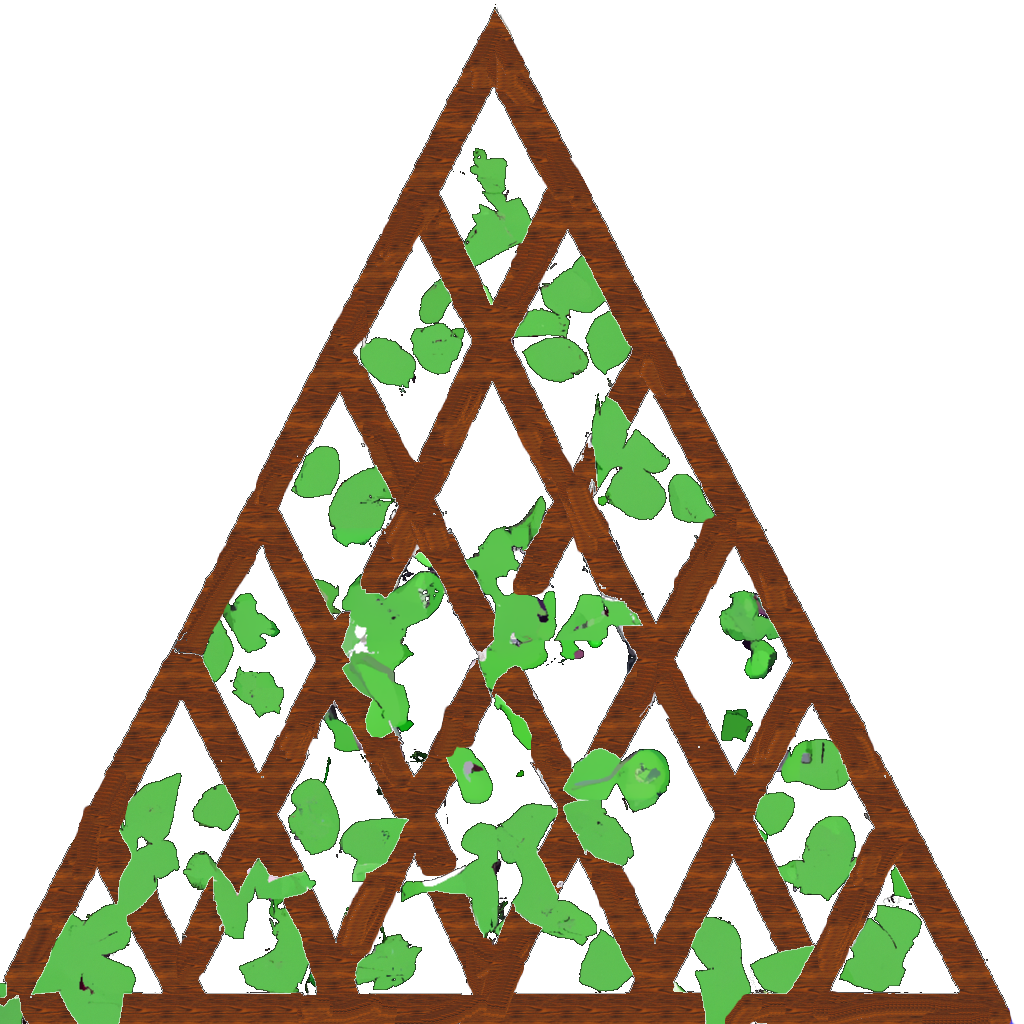
\includegraphics[width=0.17\textwidth]{../figures/trellis.png} & & 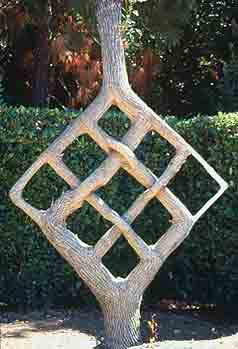
\includegraphics[width=0.12\textwidth]{../figures/grid_topiary.jpeg} & & 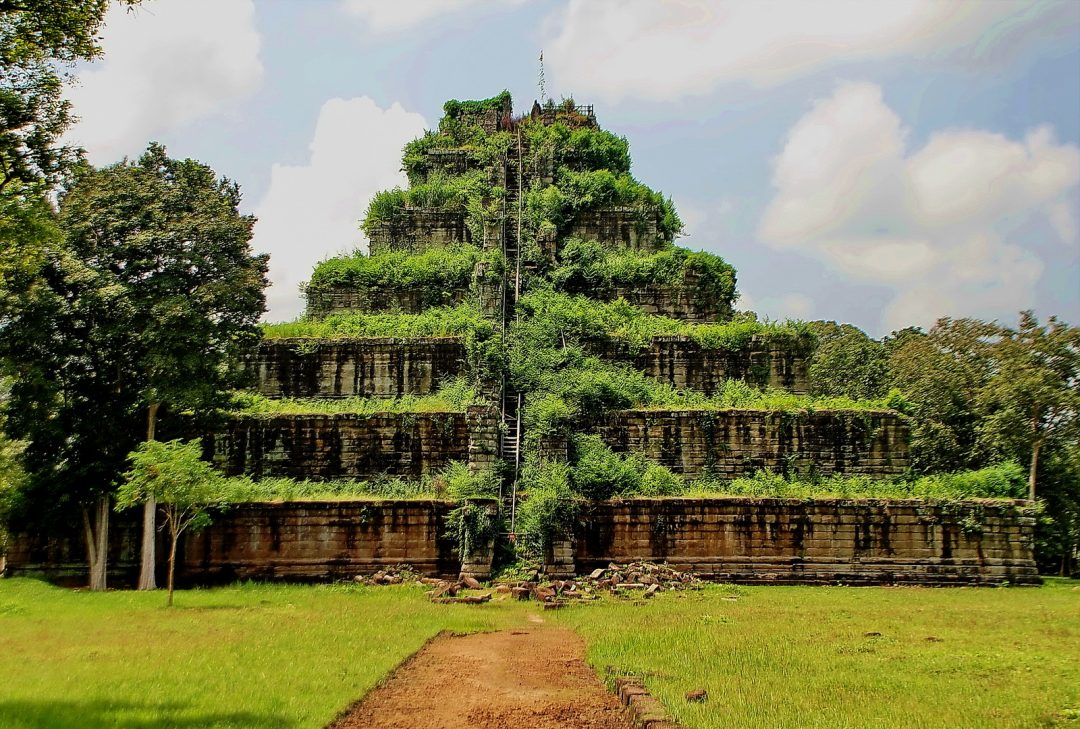
\includegraphics[width=0.23\textwidth]{../figures/tree_pyramid.jpeg} \\\\
      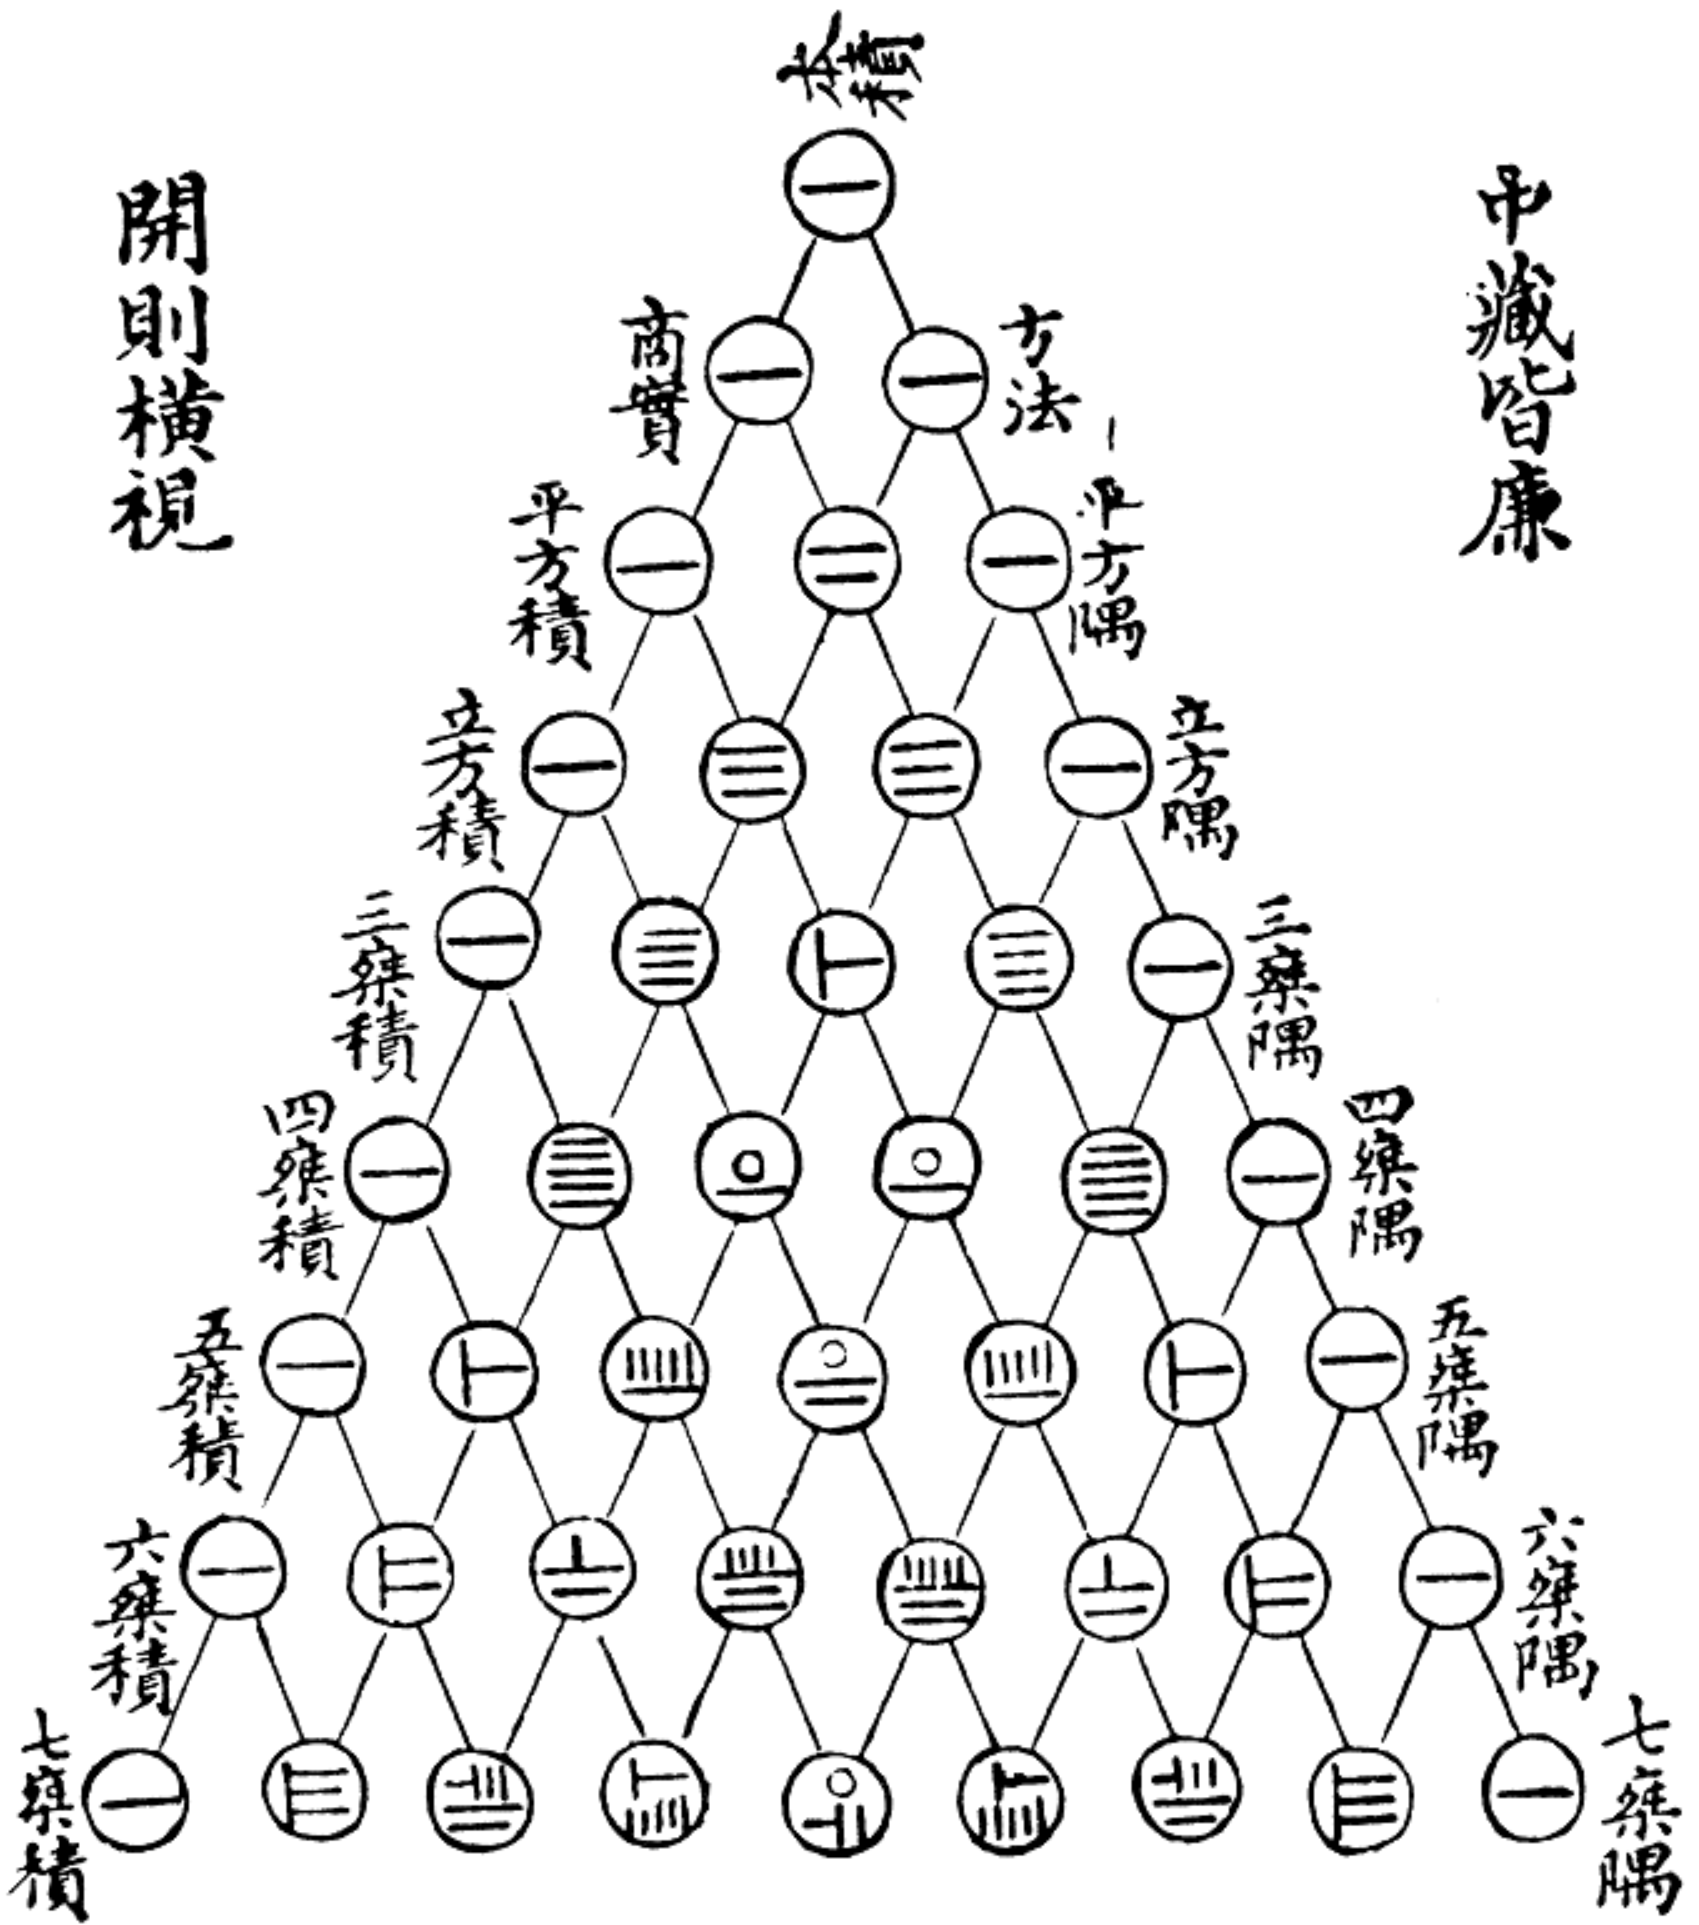
\includegraphics[width=0.17\textwidth]{../figures/jiaxian_triangle.png} & &
      \rotatebox{37}{\scalebox{0.9}{$
      \begin{pNiceMatrix}[nullify-dots,xdots/line-style=loosely dotted,delimiters-color=gray]
        \sigma_1^\shri & \Lambda & \Cdots & \Lambda^*_\sigma\\
                       & \Ddots  & \Ddots & \Vdots\\
                       &         &        & \Lambda\\
                       &         &        & \sigma_n^\shup \\
      \end{pNiceMatrix}$}} & & \scalebox{0.23}{\mkTrellis{9}}\\
      Jia Xian Triangle & & CYK Parsing & & Trellis Automaton\\
      Jia, $\sim$1030 A.D. & & Sakai, 1961 A.D. & & Dyer, 1980 A.D.\\
    \end{tabular}
  \end{center}
\end{frame}

\begin{frame}{A few observations on algebraic parsing}
  \begin{itemize}
    \item The matrix $\mathbf M^*$ is strictly upper triangular, i.e., nilpotent of degree $n$
    \item Recognizer can be translated into a parser by storing backpointers\\\\
  \end{itemize}\vspace{0.2cm}
  \begin{tabular}{ c c c }
    \small{$\mathbf{M}_1 = \mathbf{M}_0 + \mathbf{M}_0^2$} & \small{$\mathbf{M}_2 = \mathbf{M}_1 + \mathbf{M}_1^2$} & \small{$\mathbf{M}_3 = \mathbf{M}_2 + \mathbf{M}_2^2 = \mathbf{M}_4$} \\
    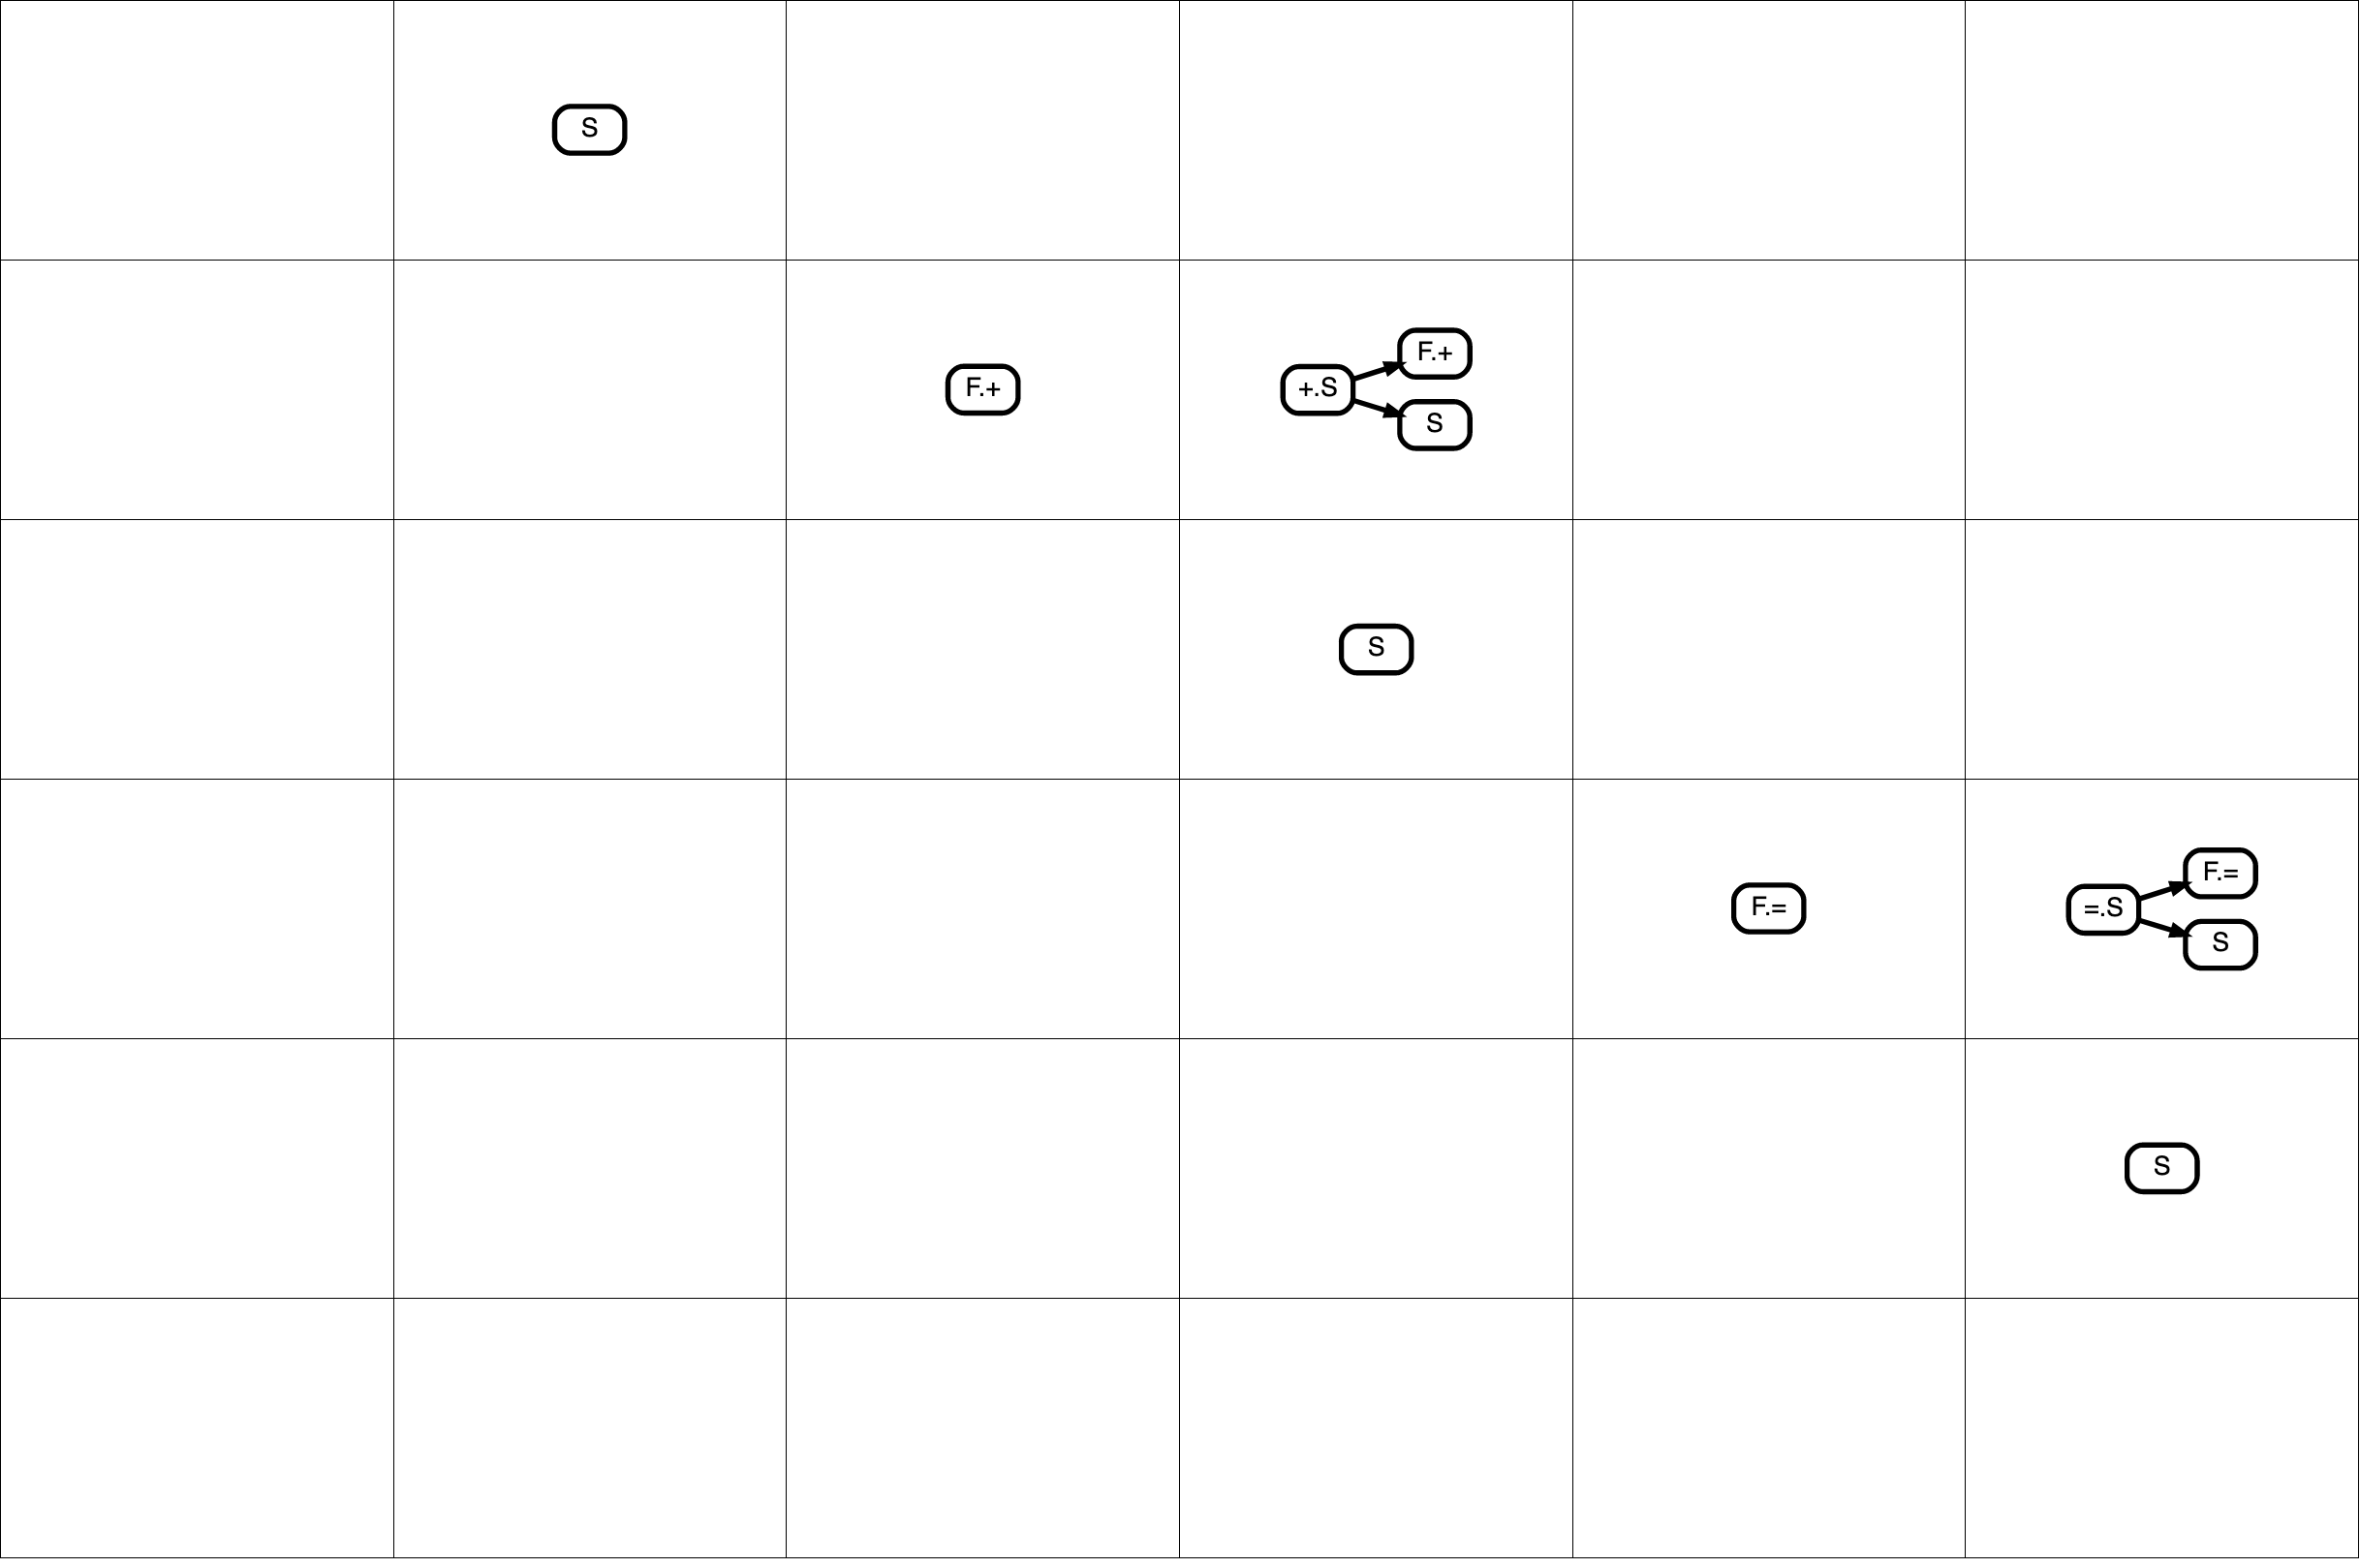
\includegraphics[trim=420 288 0 0,clip, width=3.6cm]{../figures/parse2.png} &
    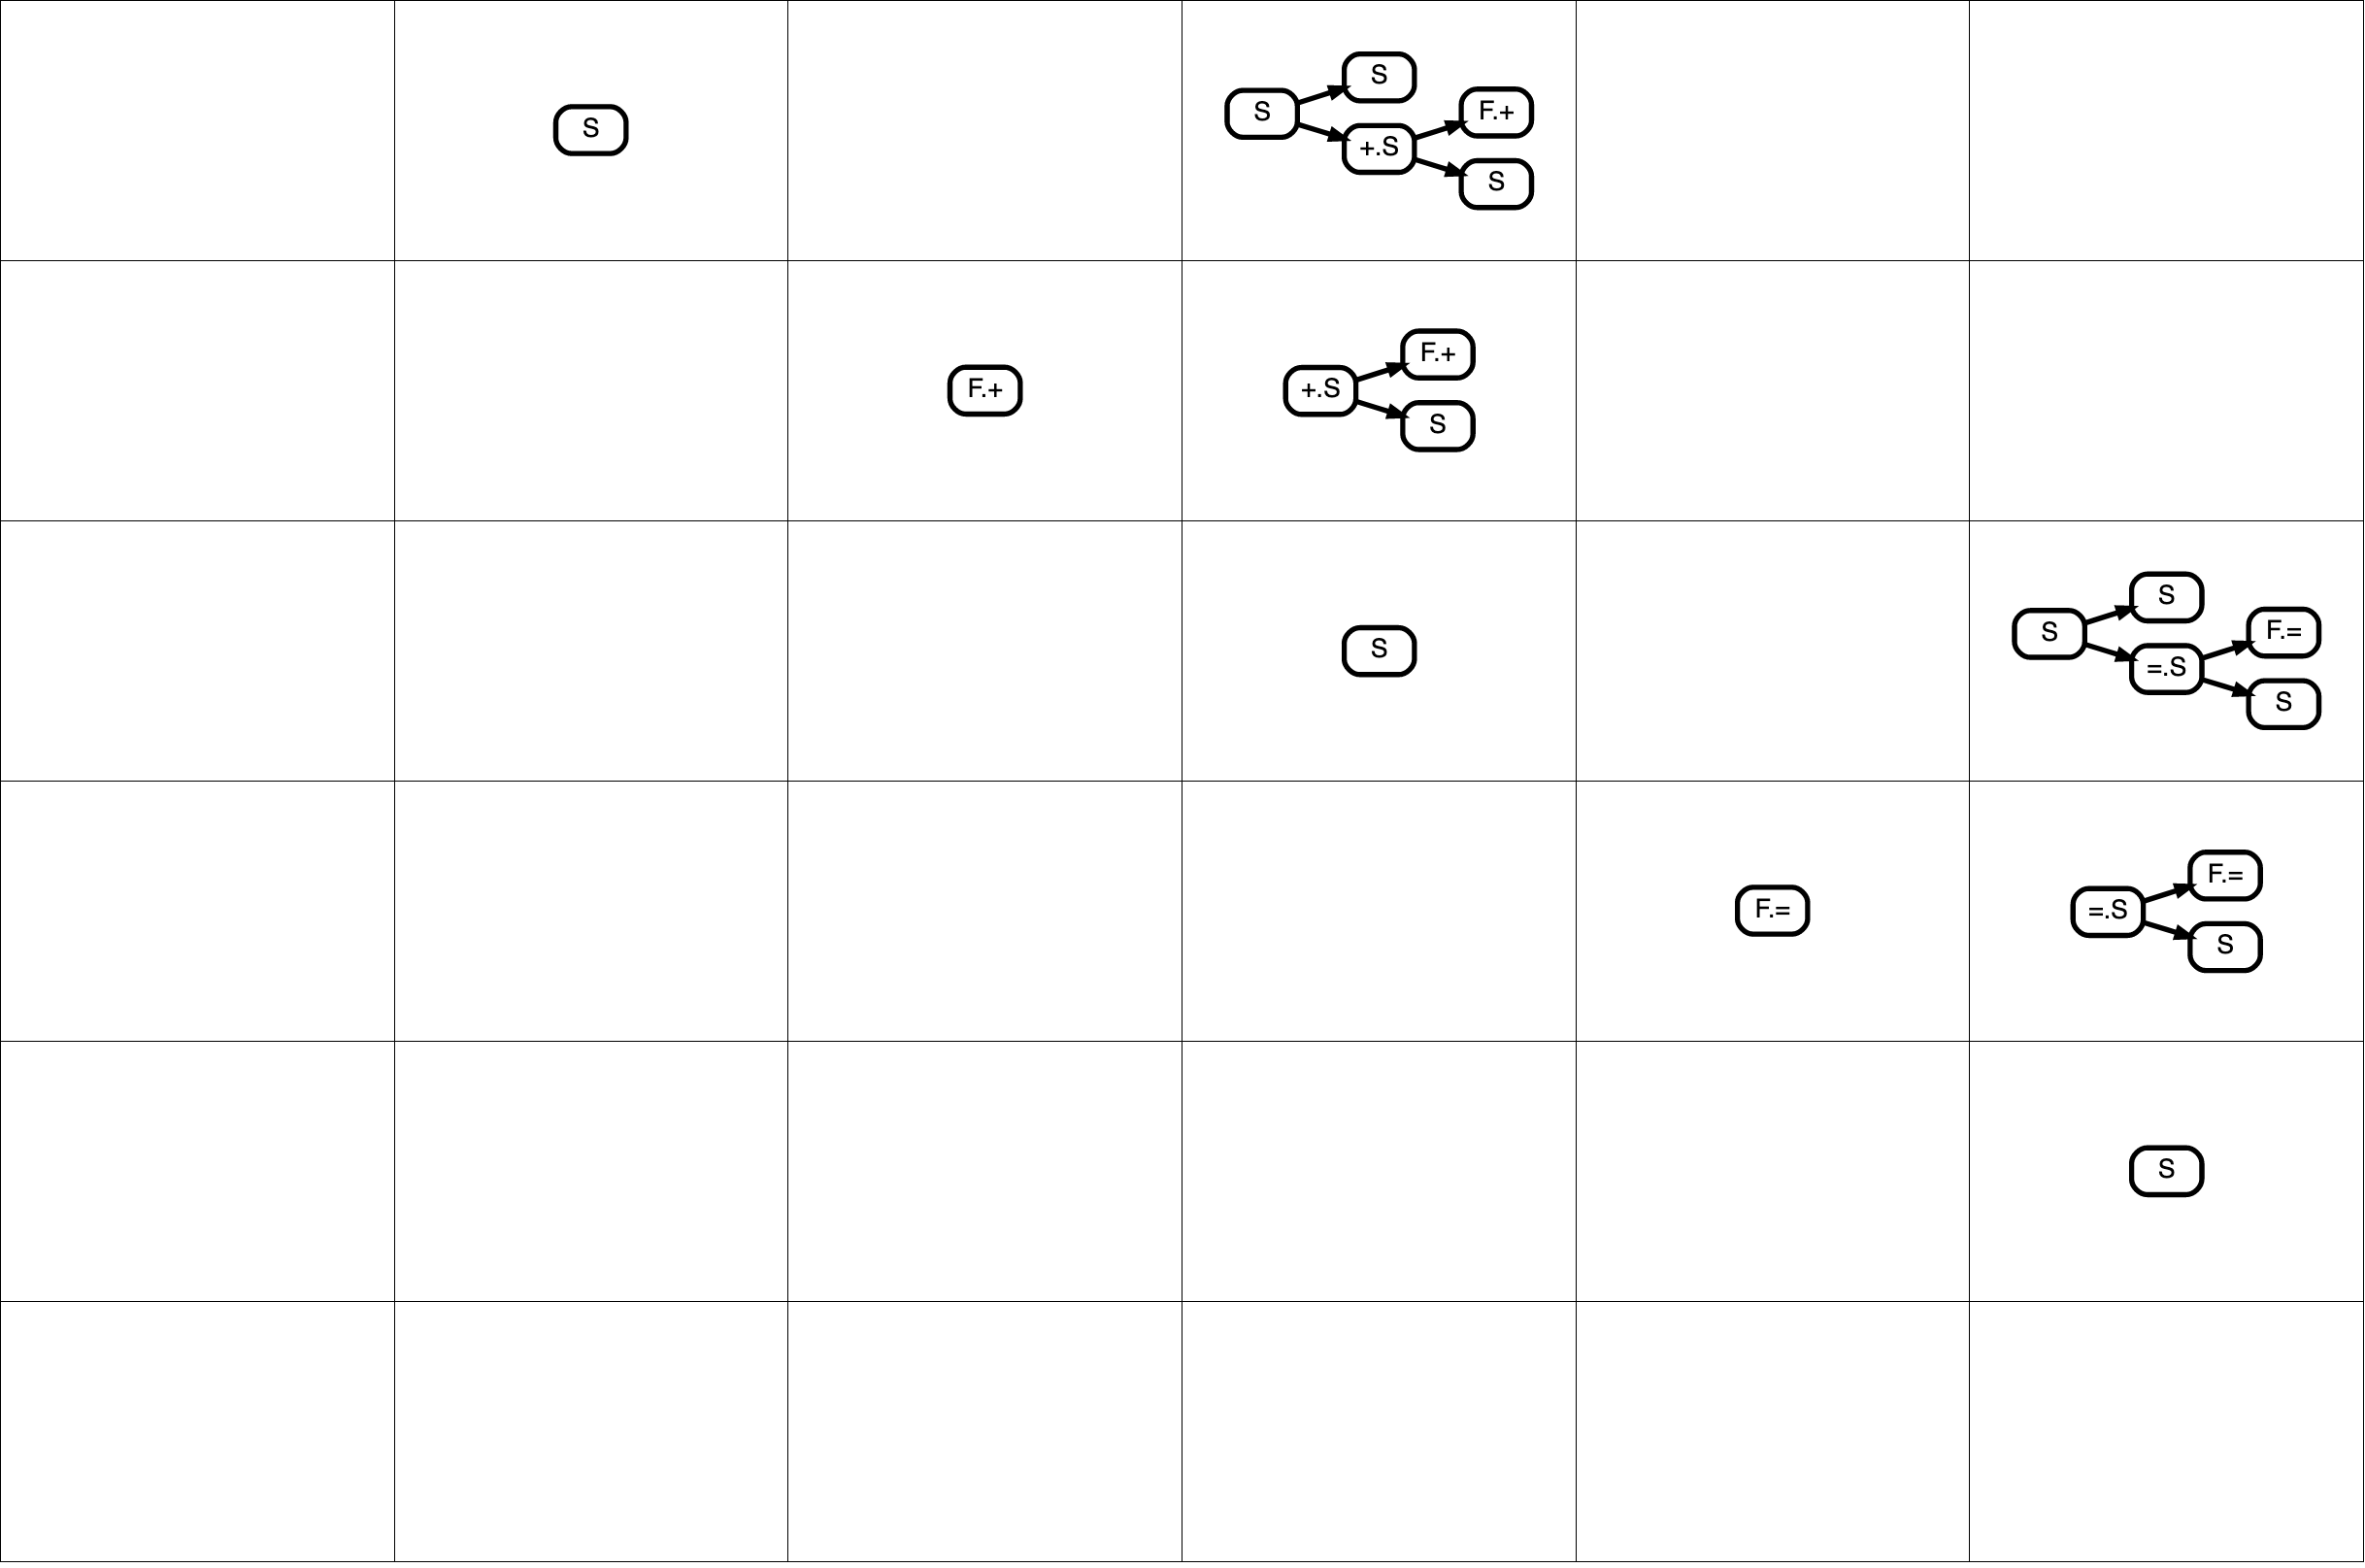
\includegraphics[trim=420 285 0 0,clip, width=3.6cm]{../figures/parse3.png} &
    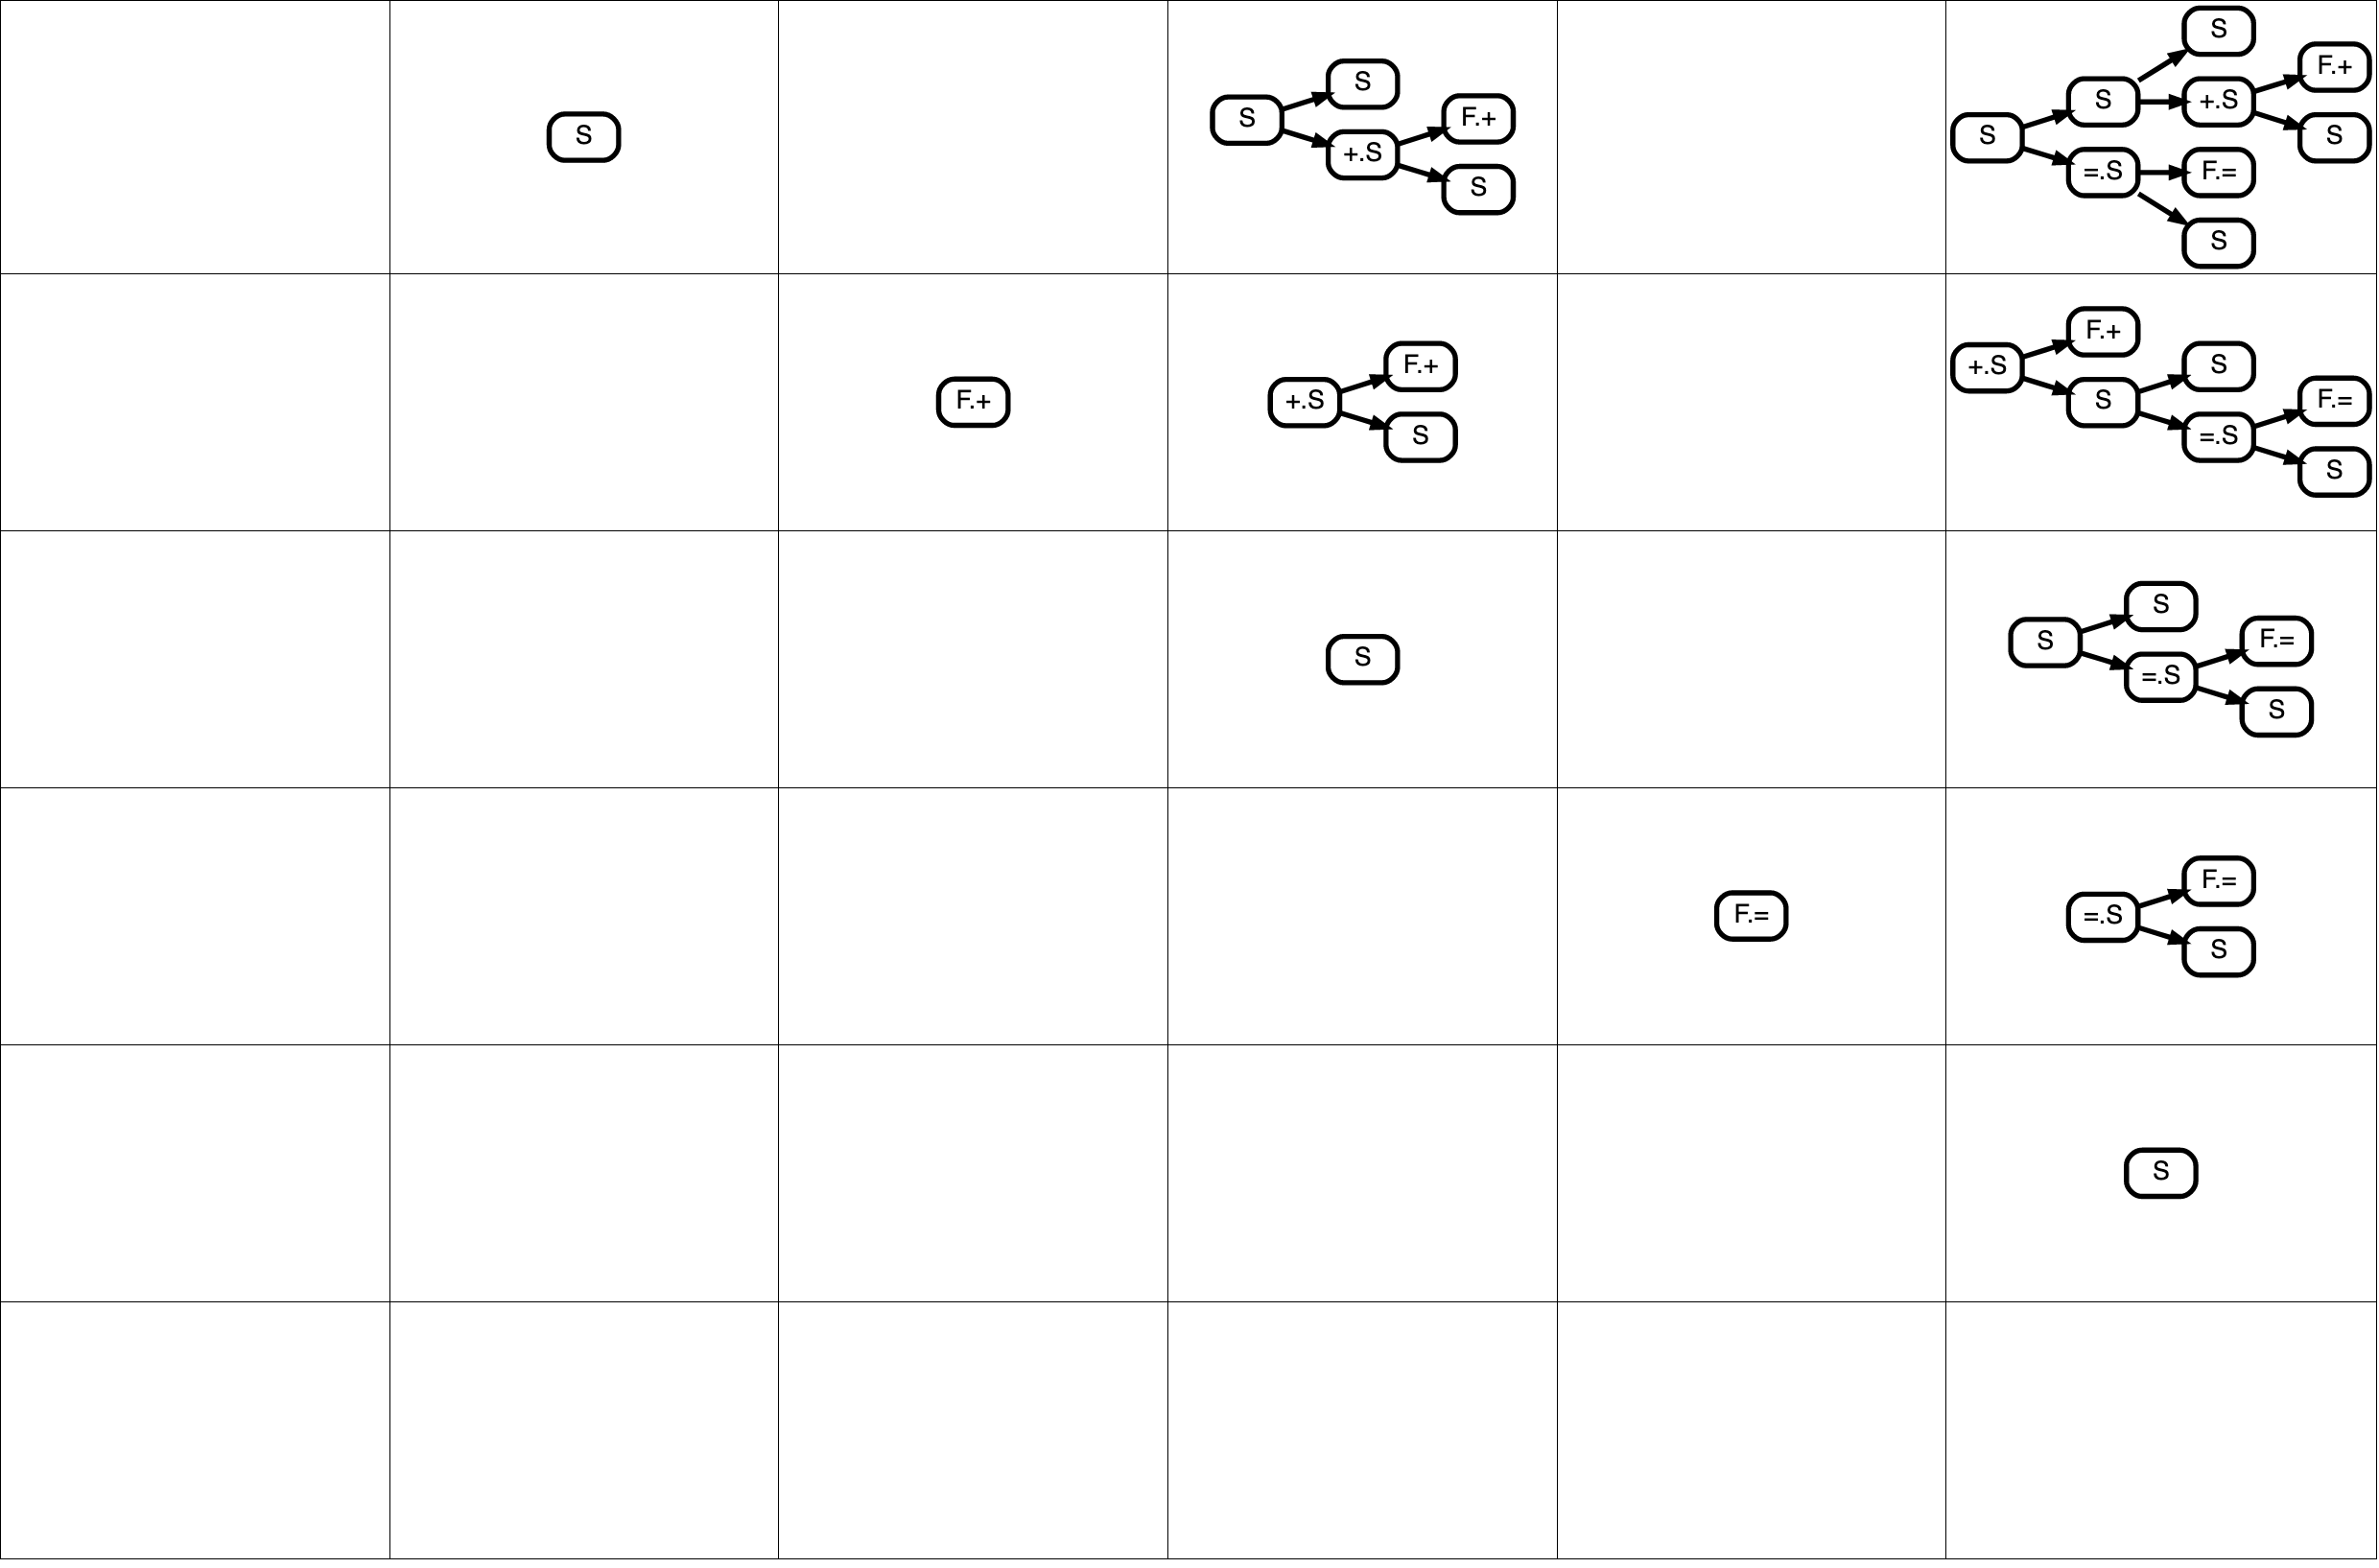
\includegraphics[trim=420 287 0 0,clip, width=3.63cm]{../figures/parse4.png}
  \end{tabular}
  \begin{itemize}
    \item The $\otimes$ operator is \textit{not} associative: $S \otimes (S \otimes S) \neq (S \otimes S) \otimes S$
    \item Built-in error recovery: nonempty submatrices = parsable fragments
    \item \texttt{seekFixpoint \{ it + it * it \}} is sufficient but unnecessary
    \item If we had a way to solve for $\mathbf{M = M + M}^2$ directly, power iteration would be unnecessary, could solve for $\mathbf{M = M}^2$ above superdiagonal
  \end{itemize}
\end{frame}

\begin{frame}[fragile]{Satisfiability + holes (our contribution)}
  \begin{itemize}
    \item Can be lowered onto a Boolean tensor $\mathbb{B}_2^{n\times n \times |V|}$ (Valiant, 1975)
    \item Binarized CYK parser can be efficiently compiled to a SAT solver
    \item Enables sketch-based synthesis in either $\sigma$ or $\mathcal G$: just use variables!
    \item We simply encode the characteristic function, i.e. $\mathds{1}_{\subseteq V}: V\rightarrow \mathbb{Z}_2^{|V|}$
    \item $\oplus, \otimes$ are defined as $\boxplus, \boxtimes$, so that the following diagram commutes:
    \[\begin{tikzcd}
        2^V \times 2^V \arrow[r, "\oplus/\otimes"] \arrow[d, "\mathds{1}^2"]
        & 2^V \arrow[d, "\mathds{1}\phantom{^{-1}}"] \\
        \mathbb{Z}_2^{|V|} \times \mathbb{Z}_2^{|V|} \arrow[r, "\boxplus/\boxtimes", labels=below] \arrow[u, "\mathds{1}^{-2}"]
        & \mathbb{Z}_2^{|V|} \arrow[u, "\mathds{1}^{-1}"]
    \end{tikzcd}\]
    \item These operators can be lifted into matrices/tensors in the usual way
    \item In most cases, only a few nonterminals are active at any given time
    \item More sophisticated representations are known for $\binom{n}{0 \leq k}$ subsets
    \item If density is desired, possible to use the Maculay representation
%            \item Set joins are an active topic of research in SQL query optimization
  \end{itemize}
\end{frame}

\begin{frame}[fragile]{Satisfiability + holes (our contribution)}
  Let us consider an example with two holes, $\sigma = 1$ \_ \_, and the grammar being $G\coloneqq\{S\rightarrow N O N, O \rightarrow + \mid \times, N \rightarrow 0 \mid 1\}$. This can be rewritten into CNF as $G'\coloneqq \{S \rightarrow N L, N \rightarrow 0 \mid 1, O \rightarrow × \mid +, L \rightarrow O N\}$. Using the algebra where $\oplus=\cup$, $X \otimes Z = \big\{\;w \mid \langle x, z\rangle \in X \times Z, (w\rightarrow xz) \in P\;\big\}$, the fixpoint $M' = M + M^2$ can be computed as follows:\\\vspace{10pt}

  \resizebox{\textwidth}{!}{
{\renewcommand{\arraystretch}{1.2}
\noindent\phantom{...}\begin{tabular}{|c|c|c|c|}
  \hline
  & $2^V$ & $\mathbb{Z}_2^{|V|}$ & $\mathbb{Z}_2^{|V|}\rightarrow\mathbb{Z}_2^{|V|}$\\\hline
  $M_0$ & \begin{pmatrix}
  \phantom{V} & \tiny{\{N\}} &         &             \\
              &              & \{N,O\} &             \\
              &              &         & \{N,O\} \\
              &              &         &
  \end{pmatrix} & \begin{pmatrix}
  \phantom{V} & \ws\bs\ws\ws &              &              \\
              &              & \ws\bs\bs\ws &              \\
              &              &              & \ws\bs\bs\ws \\
              &              &              &
  \end{pmatrix} & \begin{pmatrix}
     \phantom{V} & V_{0, 1} &          &          \\
                 &          & V_{1, 2} &          \\
                 &          &          & V_{2, 3} \\
                 &          &          &
  \end{pmatrix} \\\hline
  $M_1$ & \begin{pmatrix}
  \phantom{V} & \tiny{\{N\}} & \varnothing &         \\
              &              & \{N,O\}     & \{L\}   \\
              &              &             & \{N,O\} \\
              &              &             &
  \end{pmatrix} & \begin{pmatrix}
  \phantom{V} & \ws\bs\ws\ws & \ws\ws\ws\ws &              \\
              &              & \ws\bs\bs\ws & \bs\ws\ws\ws \\
              &              &              & \ws\bs\bs\ws \\
              &              &              &
  \end{pmatrix} & \begin{pmatrix}
                   \phantom{V} & V_{0, 1} & V_{0, 2} &          \\
                   &          & V_{1, 2} & V_{1, 3} \\
                   &          &          & V_{2, 3} \\
                   &          &          &
  \end{pmatrix} \\\hline
  $M_\infty$ & \begin{pmatrix}
  \phantom{V} & \tiny{\{N\}} & \varnothing & \{S\}   \\
              &              & \{N,O\}     & \{L\}   \\
              &              &             & \{N,O\} \\
              &              &             &
  \end{pmatrix} & \begin{pmatrix}
  \phantom{V} & \ws\bs\ws\ws & \ws\ws\ws\ws & \ws\ws\ws\bs \\
              &              & \ws\bs\bs\ws & \bs\ws\ws\ws \\
              &              &              & \ws\bs\bs\ws \\
              &              &              &
  \end{pmatrix} & \begin{pmatrix}
                   \phantom{V} & V_{0, 1} & V_{0, 2} & V_{0, 3} \\
                   &          & V_{1, 2} & V_{1, 3} \\
                   &          &          & V_{2, 3} \\
                   &          &          &
  \end{pmatrix}\\\hline
\end{tabular}
}
  }
\end{frame}

\begin{frame}[fragile]{Chomsky Denormalization}
  Chomksy normalization is needed for matrix-based parsing, however produces lopsided parse trees. We can denormalize them using a simple recusive procedure to restore the natural shape of the original CFG:\vspace{0.5cm}\\

  \begin{minipage}[l]{6cm}
    \vspace{0.3cm}\resizebox{\textwidth}{!}{
      \begin{tabular}{ll}
        \Tree [.\texttt{S} \tikz\node(v1){\texttt{true}} [.$\ccancel{\texttt{and.S}}$ \tikz\node(v3){\texttt{and}} [.\texttt{S} \tikz\node(v5){\texttt{(}} [.$\ccancel{\texttt{S.)}}$ [.\texttt{S} \tikz\node(v9){\texttt{false}} [.$\ccancel{\texttt{or.S}}$ \tikz\node(v11){\texttt{or}} [.\texttt{S} \texttt{!} \texttt{true} ] ] ] \tikz\node(v7){\texttt{)}} ] ] ] ]
%    \Tree [.S [.NP John ] [.VP [.\tikz\node(v1){V}; sleeps ] ] ]
        \hspace{-2cm}
        &
        \Tree [.\texttt{S} \tikz\node(v2){\texttt{true}} \tikz\node(v4){\texttt{and}} [.\texttt{S} \tikz\node(v6){\texttt{(}} [.\texttt{S} \tikz\node(v10){\texttt{false}} \tikz\node(v12){\texttt{or}} [.\texttt{S} \texttt{!} \texttt{true} ] ] \tikz\node(v8){\texttt{)}} ] ]\\\\
%    \Tree [.\tikz\node(v2){V}; [.\tikz\node(v3){V}; ] [.Adv {a lot} ] ]
        \hspace{1cm}\huge{Pre-Denormalization} & \hspace{3cm}\huge{Post-Denormalization}
      \end{tabular}
      \begin{tikzpicture}[overlay]
%    \draw [red,dashed,-stealth] (v1) to[bend left] (v2);
        \draw [red,dashed,-stealth] (v3) to[bend left] (v4);
%    \draw [red,dashed,-stealth] (v5) to[bend left] (v6);
        \draw [red,dashed,-stealth] (v7) to[bend left] (v8);
%    \draw [red,dashed,-stealth] (v9) to[bend right] (v10);
        \draw [red,dashed,-stealth] (v11) to[bend right] (v12);
      \end{tikzpicture}
    }
%    \caption{Result of applying Algorithm~\ref{alg:cap} to the tree obtained by parsing the string: \texttt{true and ( false or ! true )}.}
  \end{minipage}
  \hspace{-0.7cm}\scalebox{0.6}{
    \begin{minipage}[l]{10cm}
  \begin{algorithm}[H]
    \caption{Rewrite procedure for tree denormalization}\label{alg:cap}
    \begin{algorithmic}
      \Procedure{Denormalize}{\texttt{t: Tree}}
        \State $\texttt{stems} \leftarrow \{\:\textsc{Denormalize}(\texttt{c}) \mid \texttt{c} \in \texttt{t.children}\:\}$
        \If{$\texttt{t.root} \in V_{\mathcal{G}'} \setminus V_{\mathcal{G}}$}
          \State \textbf{return } \texttt{stems} \Comment{Drop synthetic nonterminals.}
        \Else\Comment{Graft the denormalized children on root.}
        \State \textbf{return } $\{\:\texttt{Tree(root, stems)}\:\}$
        \EndIf
      \EndProcedure
    \end{algorithmic}
  \end{algorithm}
  \end{minipage}
}

\vspace{1cm}All synthetic nonterminals are excised during Chomsky denormalization. Rewriting improves legibility but does not alter the underlying semantics.
\end{frame}

\begin{frame}[fragile]{Incremental parsing}
  Should only need to recompute submatrices affected by individual edits. In the worst case, each edit requires quadratic complexity in terms of $|\Sigma^*|$, assuming $\mathcal{O}(1)$ cost for each CNF-nonterminal subset join, $\mathbf{V}'_1\otimes \mathbf{V}'_2$.
  \begin{center}
    \begin{tabular}{ c c c c c }
      \scalebox{0.32}{\mkTrellisAppend{7}} & & \scalebox{0.32}{\mkTrellisInsert{6}}         & & \scalebox{0.32}{\mkTrellisInsert{7}}         \\
      Append                               & & Delete                                       & & Insert                                       \\
      $\mathcal{O}(n+1)$                     & & $\mathcal{O}\left(\frac{1}{4}(n-1)^2\right)$ & & $\mathcal{O}\left(\frac{1}{4}(n+1)^2\right)$ \\
    \end{tabular}
  \end{center}
  Related to \textbf{dynamic matrix inverse} and \textbf{incremental transitive closure} with vertex updates. With a careful encoding, we can incrementally update SAT constraints as new keystrokes are received to eliminate redundancy.
\end{frame}

%\begin{frame}{Error Recovery}
%  \begin{figure}[H]
%    \adjustbox{scale=0.75,center}{%
%    \hspace{-0.5cm}\begin{minipage}[l]{6cm}
%      \[
%        \begin{NiceMatrix}
%              \leftarrow & \nse & \nsi & \nfi & \nfo & \nth & \ntw & \non & \leftarrow & \ppp \\
%                         &      & \ddd & \ddd & \ddd & \ddd & \ddd & \ddd & \ddd & \ppp \\
%          \sigma_1^\shri & \cdd &      & A    &      &      &      &      &      & \ppp \\
%                    \vno & \ddd &  T_A & \vdd &      &      &      &      &      & \ppp \\
%                    \vdd & \ddd &      & \pcd & \cdd &      & B    &      &      & \ppp \\
%                         &      &      &      &      & T_B  & \vdd &      &      & \ppp \\
%                         &      &      &      &      &      & \pcd & \cdd &      & C    \\
%                         &      &      &      &      &      &      &      & T_C  & \vdd \\
%                         &      &      &      &      &      &      & \text{\emoji{cross-mark}} &      & \\
%                         &      &      &      &      &      &      &      &      & \\
%                         &      &      &      &      &      &      &      &      & \\
%                         &      &      &      &      &      &      &      & \ppp & \sigma_n^\shup \\
%                    \vno & \cdd &      &      &      &      &      &      & \vno &
%        \end{NiceMatrix}
%      \]
%    \end{minipage}
%    }
%    \hspace{1cm}
%
%    \caption{By recursing over upper diagonals of decreasing elevation and discarding subtrees that fall under the shadow of another's canopy, we can recover parseable subtrees.}
%  \end{figure}
%\end{frame}

\begin{frame}[fragile]{Conjunctive parsing}
  It is well-known that the family of CFLs is not closed under intersection. For example, consider $\mathcal{L}_\cap := \mathcal{L}_{\mathcal{G}_1} \cap \mathcal{L}_{\mathcal{G}_2}$:

  \begin{table}[H]
    \begin{tabular}{llll}
      $P_1 := \big\{\;S \rightarrow L R,$ & $L \rightarrow a b \mid a L b,$ & $R \rightarrow c \mid c R\;\big\}$\vspace{5pt} \\
      $P_2 := \big\{\;S \rightarrow L R,$ & $R \rightarrow b c \mid b R c,$ & $L \rightarrow a \mid a L\;\big\}$
    \end{tabular}
  \end{table}

  \noindent Note that $\mathcal{L}_\cap$ generates the language $\big\{\;a^d b^d c^d \mid d > 0\;\big\}$, which according to the pumping lemma is not context-free. To encode $\mathcal{L}_\cap$, we intersect all terminals $\Sigma_\cap := \bigcap_{i=1}^c \Sigma_i$, then for each $t_\cap \in \Sigma_\cap$ and CFG, construct an equivalence class $E(t_\cap, \mathcal{G}_i) = \{ w_i \mid (w_i \rightarrow t_\cap) \in P_i\}$ as follows:\vspace{-5pt}

  \begin{align}
    \bigwedge_{t\in\Sigma_\cap}\bigwedge_{j = 1}^{c-1}\bigwedge_{i=1}^{|\sigma|} E(t_{\cap}, \mathcal{G}_j) \equiv_{\sigma_i} E(t_{\cap}, \mathcal{G}_{j+1})
  \end{align}
  % Generated by cfl4_intersection.vox, open with https://voxelator.com/
  \begin{figure}[H]
    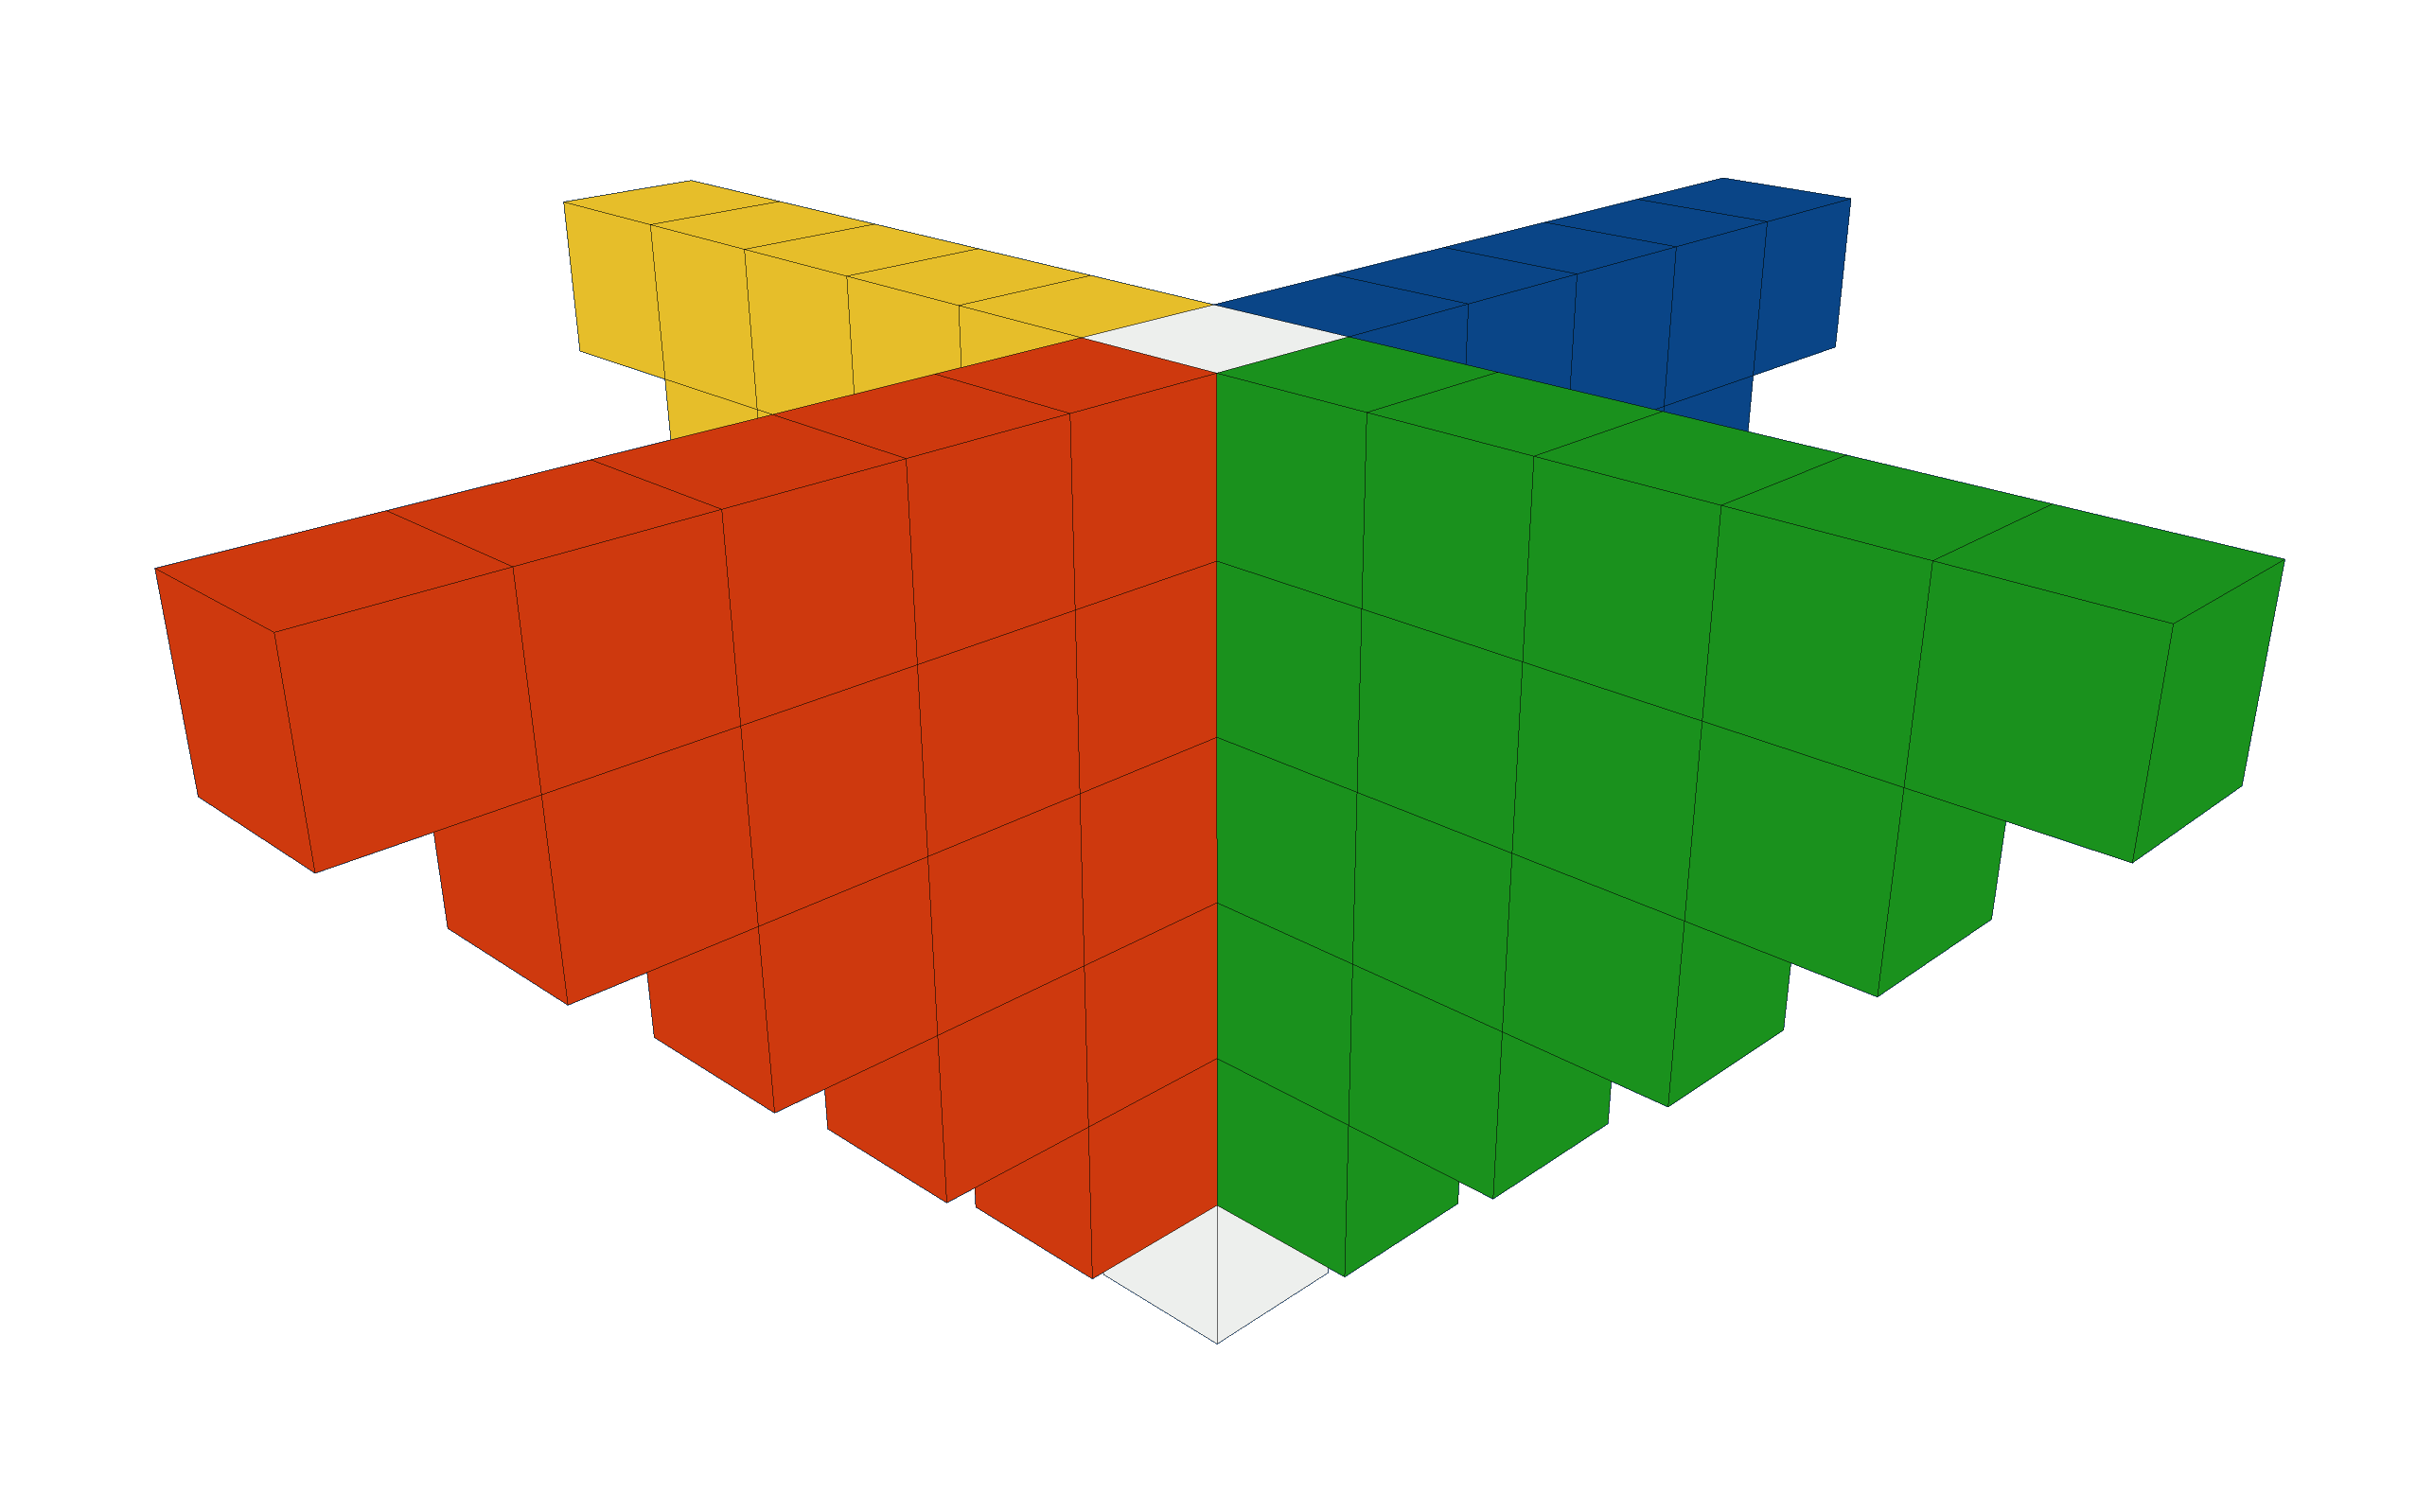
\includegraphics[height=0.093\textwidth]{../figures/angle1.png}\hspace{-5pt}
    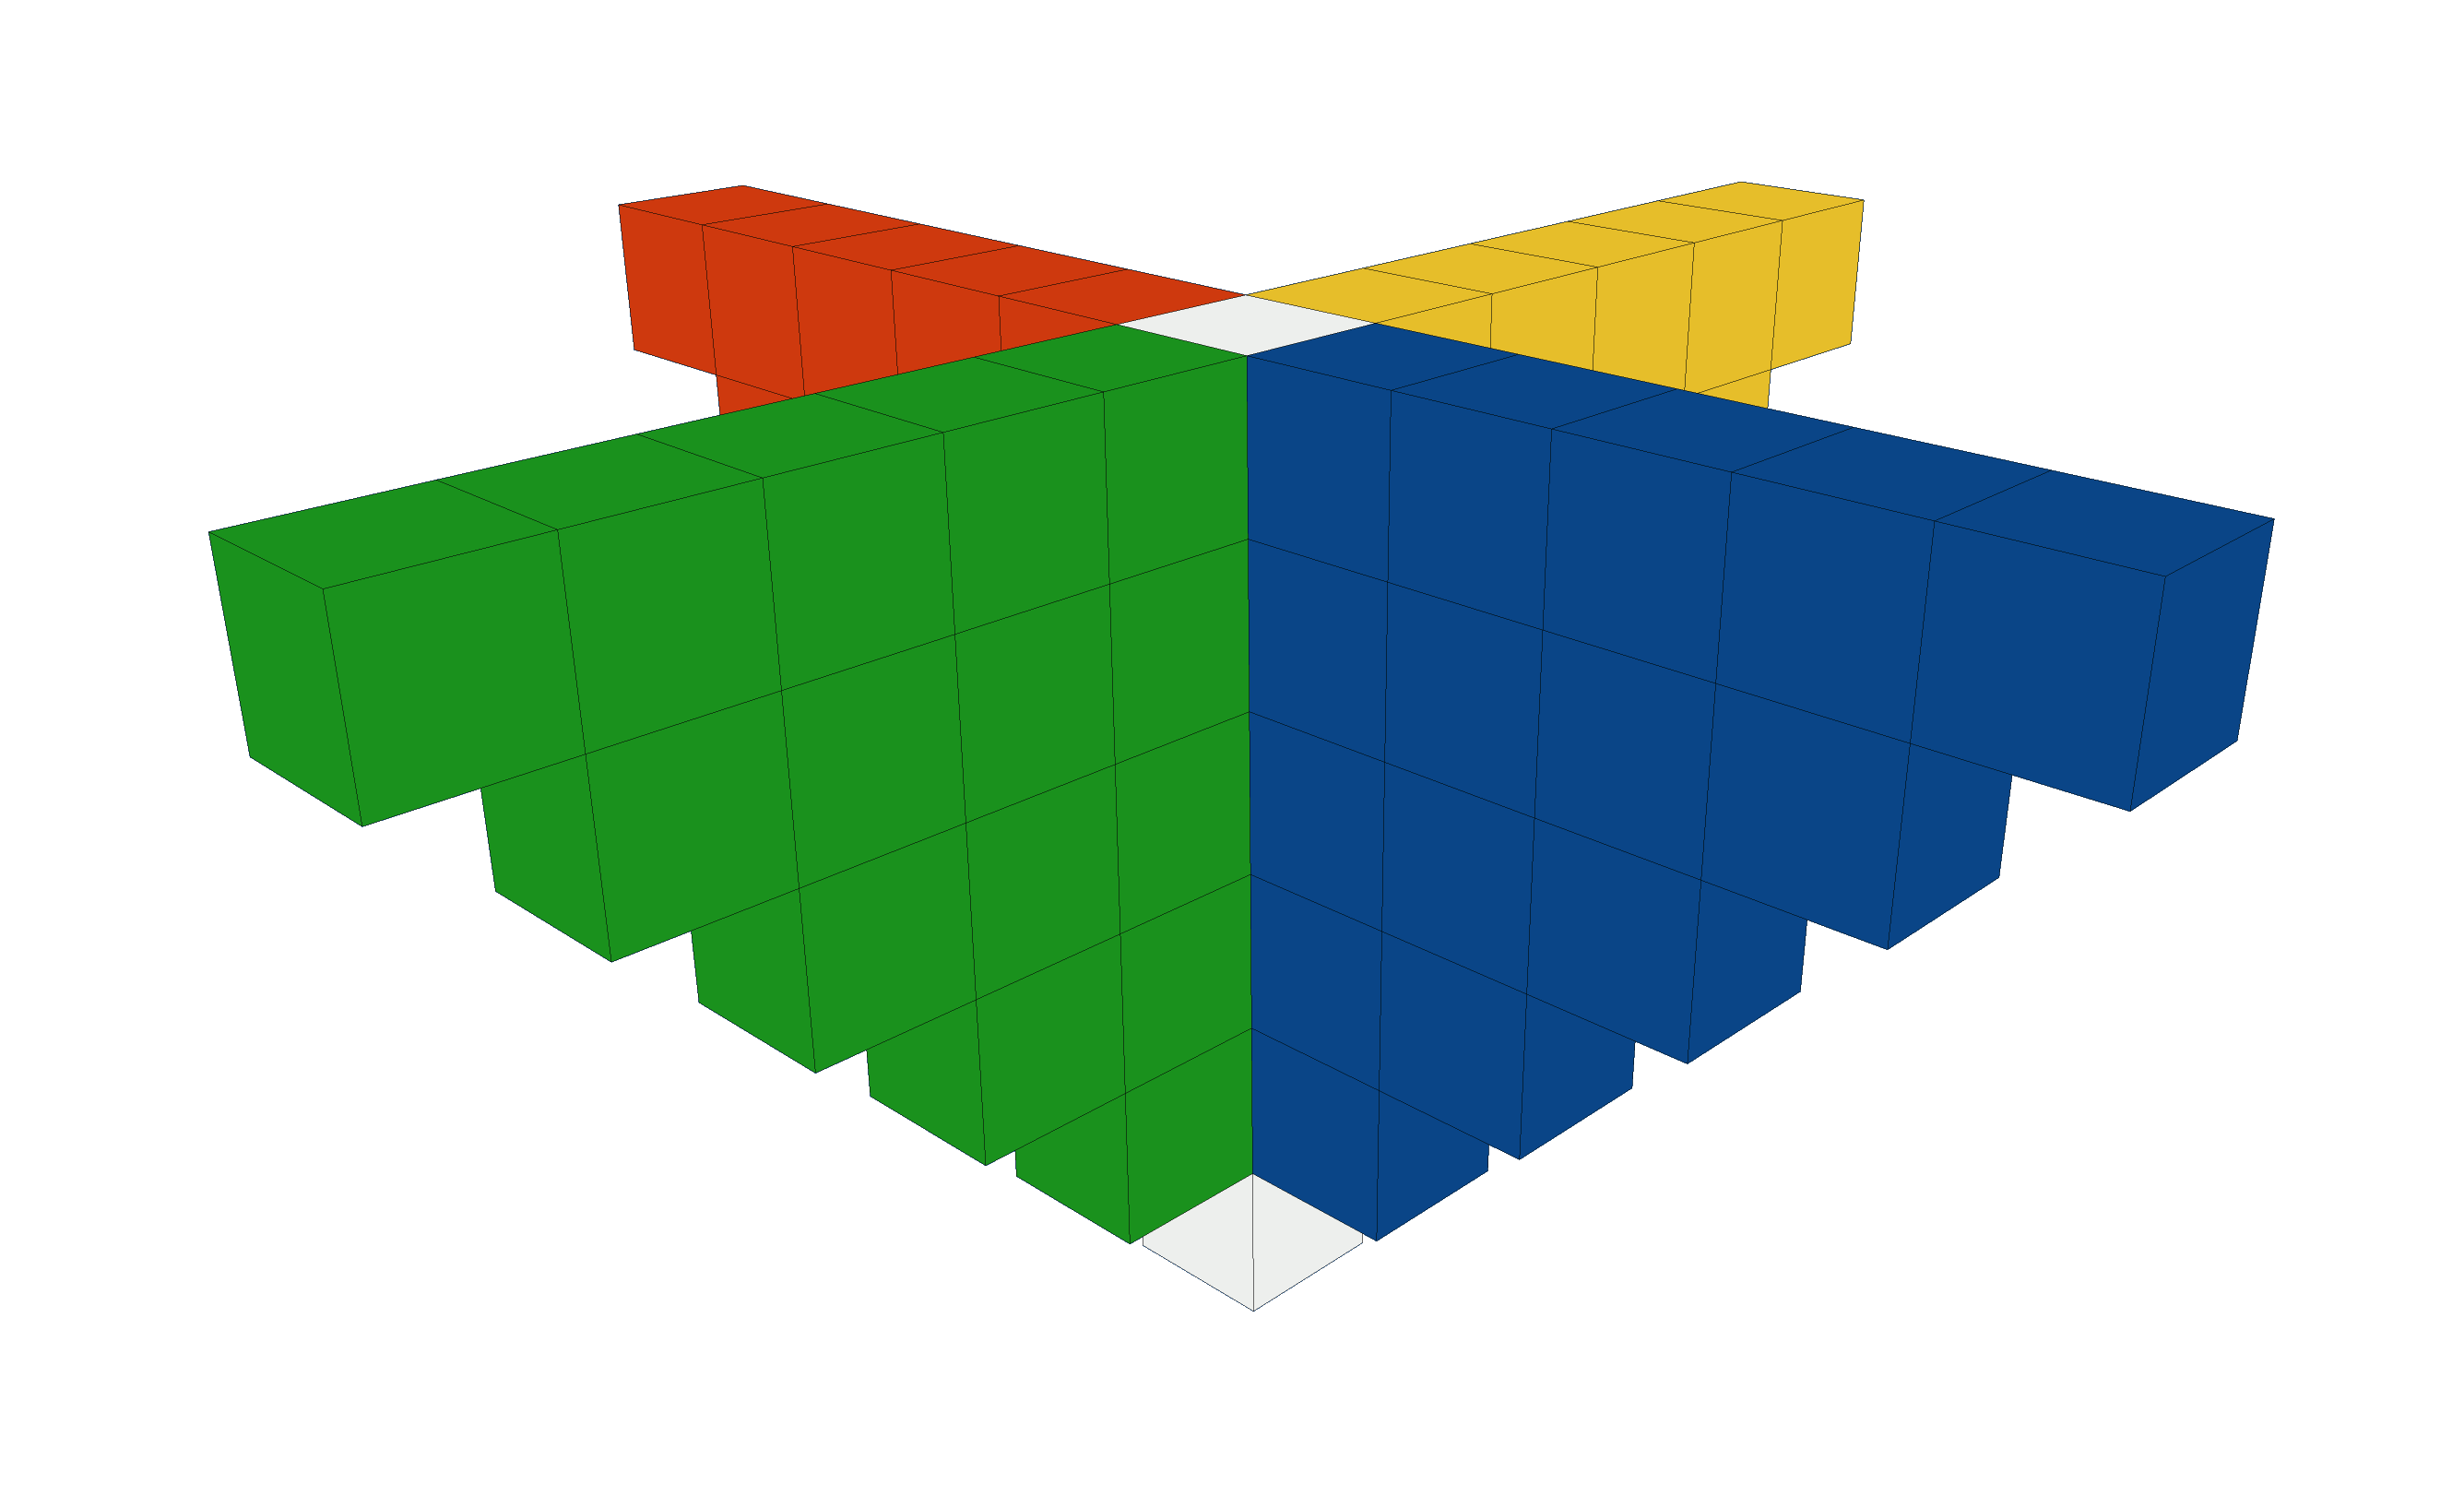
\includegraphics[height=0.093\textwidth]{../figures/angle2.png}\hspace{-5pt}
    
\includegraphics[height=0.093\textwidth]{../figures/angle5.png}\hspace{-5pt}
    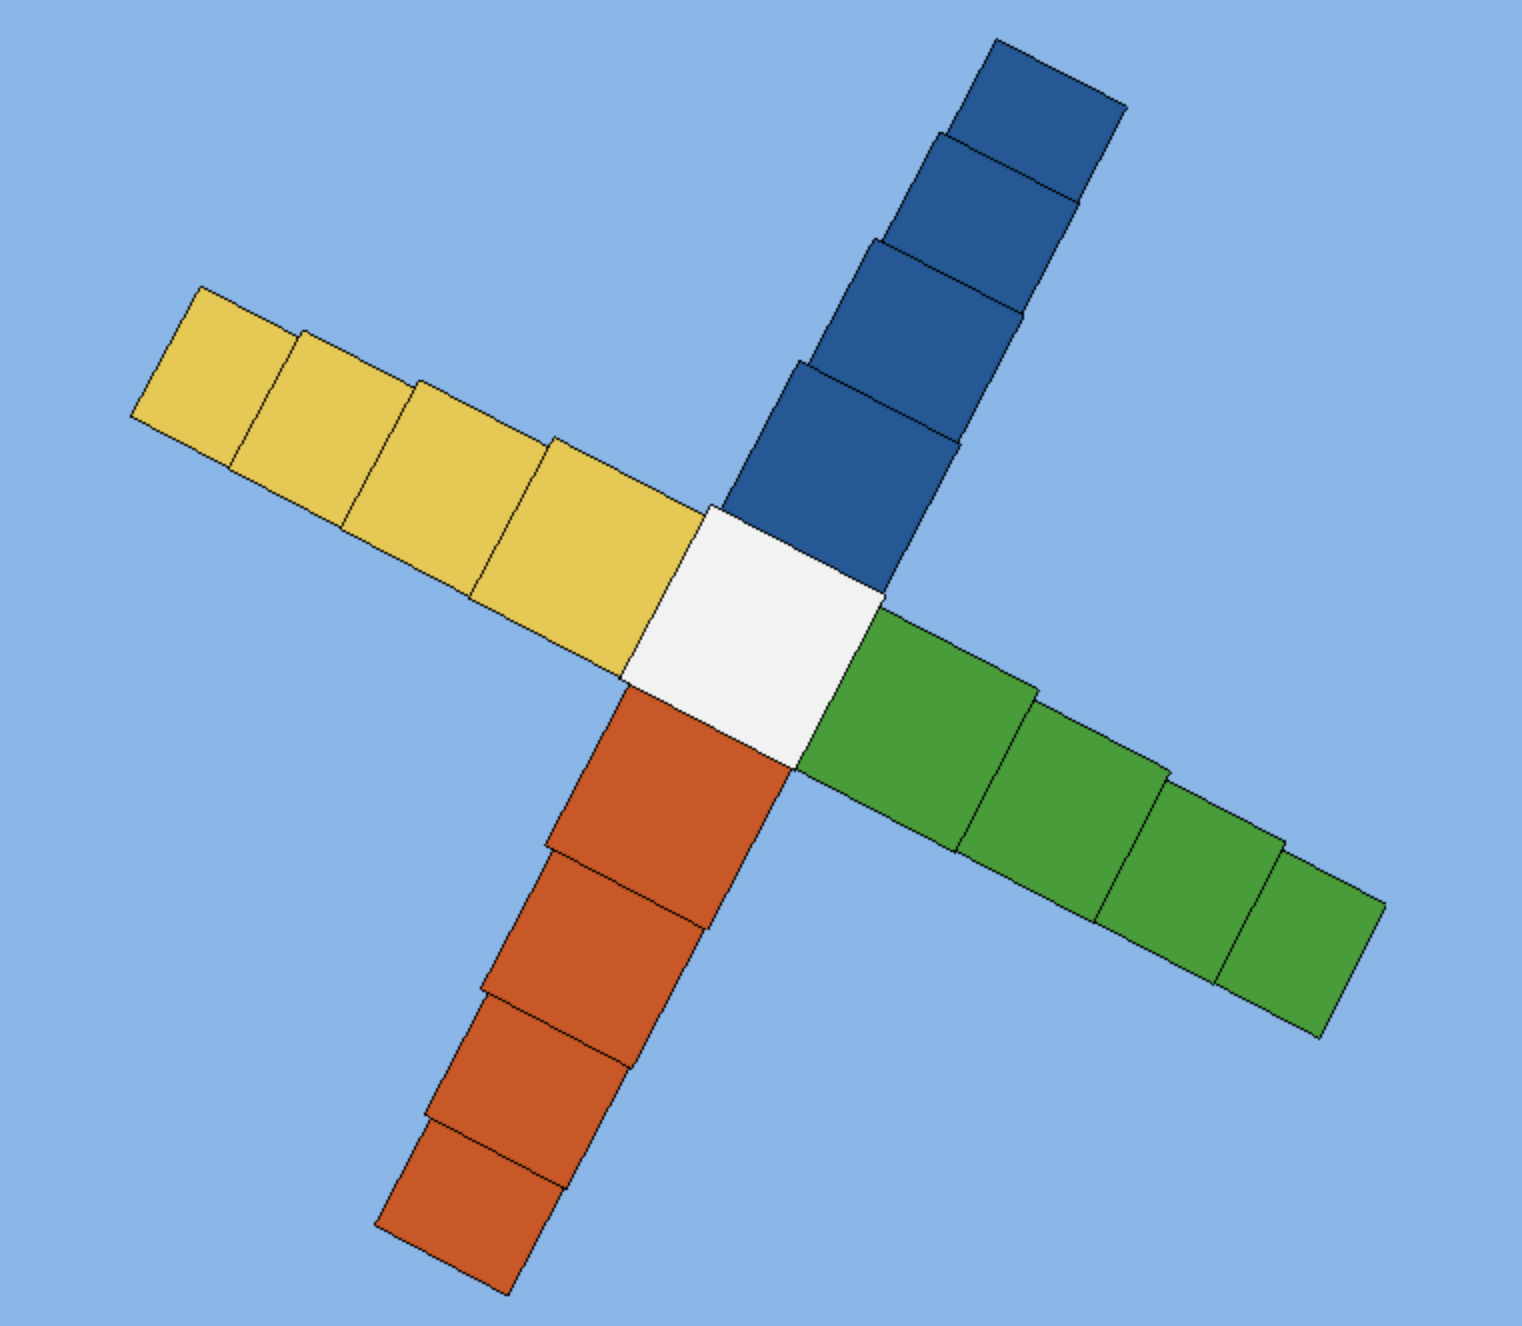
\includegraphics[height=0.093\textwidth]{../figures/angle3.png}\hspace{-3pt}
    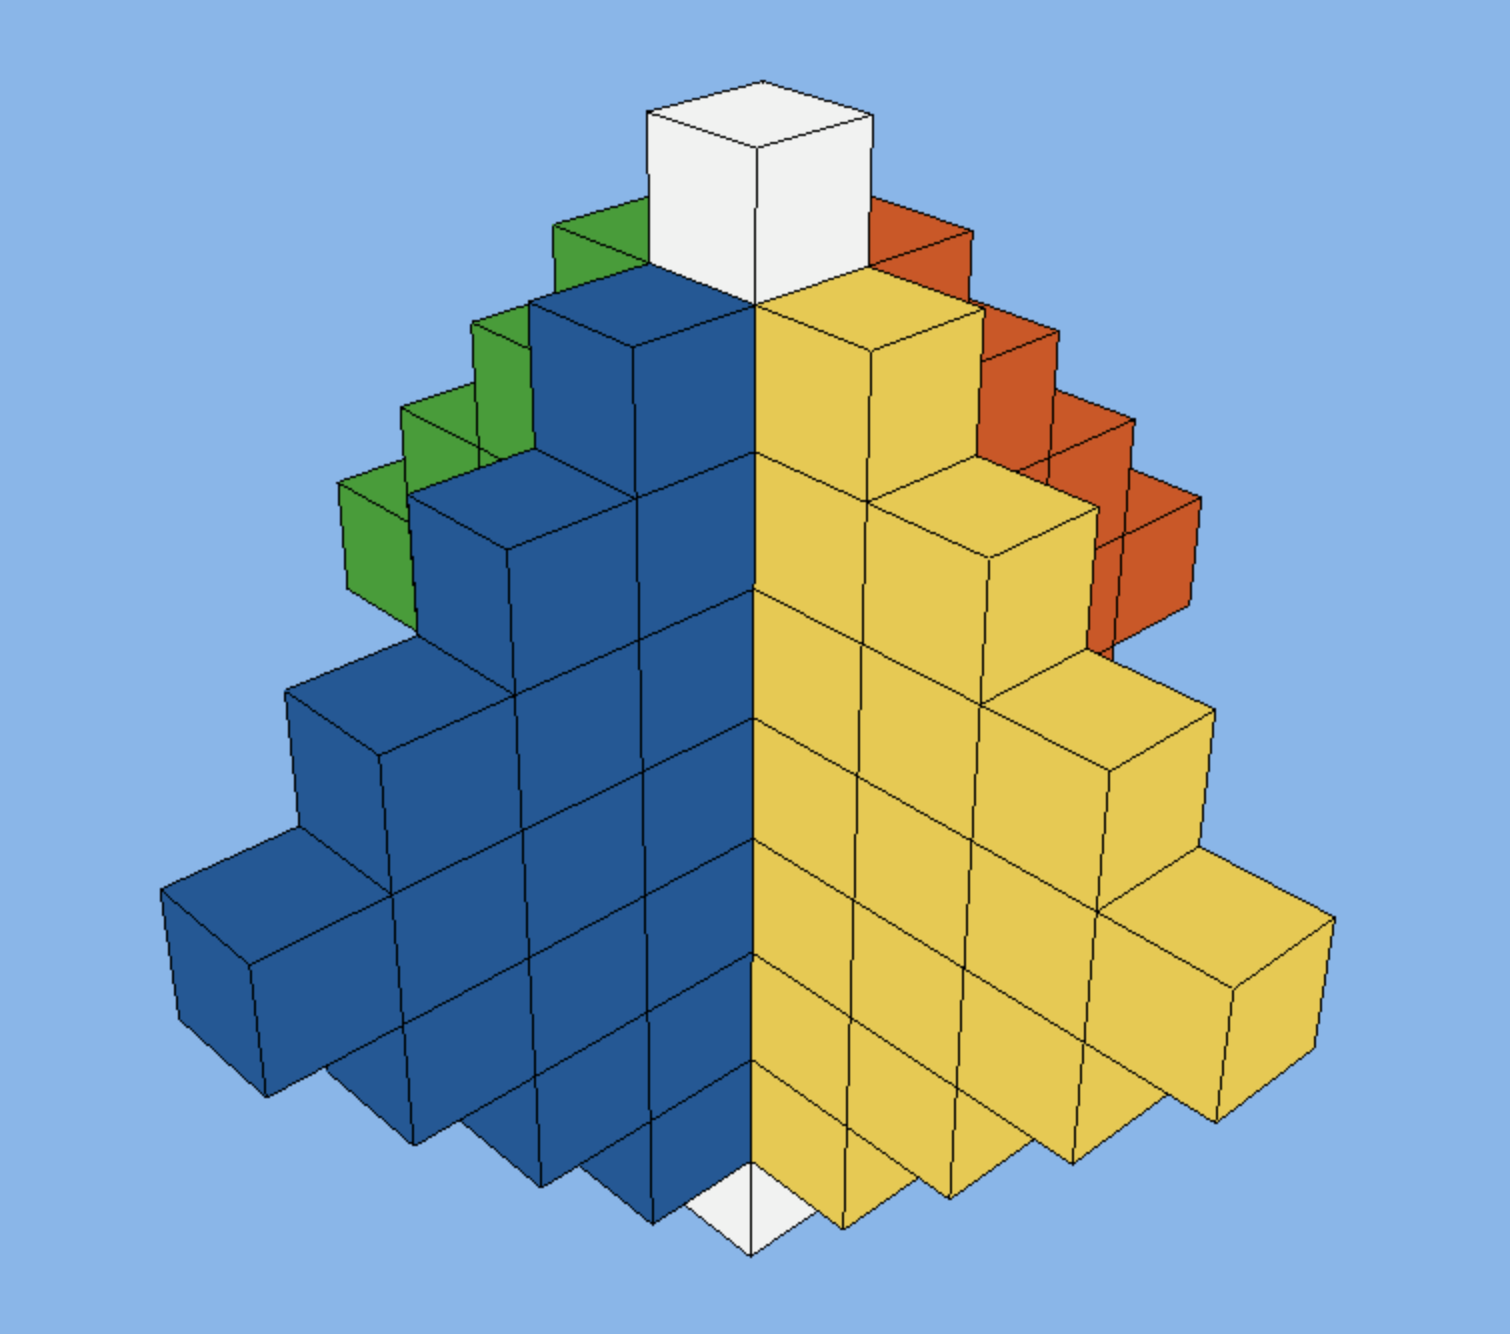
\includegraphics[height=0.093\textwidth]{../figures/angle4.png}
  \end{figure}
\end{frame}

\begin{frame}[fragile]{Levenshtein reachability and monotone infinite automata}
  \begin{figure}[H]
    \begin{minipage}[c]{0.5\textwidth}
      \centering
      \underline{MAIA}\vspace{10pt}
      \resizebox{\textwidth}{!}{
      \begin{tikzpicture}[
%->, % makes the edges directed
      >=stealth',
      node distance=2.5cm, % specifies the minimum distance between two nodes. Change if necessary.
%  every state/.style={thick, fill=gray!10}, % sets the properties for each ’state’ node
      initial text=$ $, % sets the text that appears on the start arrow
      ]
      \node[state, initial]                (00) {$q_{0,0}$};
      \node[state, right of=00]            (10) {$q_{1,0}$};
      \node[state, right of=10]            (20) {$q_{2,0}$};
      \node[state, right of=20]            (30) {$q_{3,0}$};
      \node[right of=30]                   (40) {$\vphantom{\vdots}\cdots$};
      \node[accepting, state, right of=40] (n0) {$q_{n,0}$};

      \node[state, above of=00]            (01) {$q_{0,1}$};
      \node[state, right of=01]            (11) {$q_{1,1}$};
      \node[state, right of=11]            (21) {$q_{2,1}$};
      \node[state, right of=21]            (31) {$q_{3,1}$};
      \node[right of=31]                   (41) {$\vphantom{\vdots}\cdots$};
      \node[accepting, state, right of=41] (n1) {$q_{n,1}$};

      \node[above of=01]                   (0j) {$\mathmakebox[\widthof{$\cdots$}]{\vdots}$};
\node[right of=0j]                   (1j) {$\mathmakebox[\widthof{$\cdots$}]{\vdots}$};
\node[right of=1j]                   (2j) {$\mathmakebox[\widthof{$\cdots$}]{\vdots}$};
\node[right of=2j]                   (3j) {$\mathmakebox[\widthof{$\cdots$}]{\vdots}$};
\node[right of=3j]                   (4j) {$\iddots$};
\node[accepting, right of=4j]        (nj) {$\mathmakebox[\widthof{$\cdots$}]{\vdots}$};

\node[state, above of=0j]            (0k) {$q_{0,k}$};
\node[state, right of=0k]            (1k) {$q_{1,k}$};
\node[state, right of=1k]            (2k) {$q_{2,k}$};
\node[state, right of=2k]            (3k) {$q_{3,k}$};
\node[right of=3k]                   (4k) {$\vphantom{\vdots}\cdots$};
\node[accepting, state, right of=4k] (nk) {$q_{n,k}$};

\draw [->] (00) edge[below] node{$\sigma_1$} (10);
\draw [->] (10) edge[below] node{$\sigma_2$} (20);
\draw [->] (20) edge[below] node{$\sigma_3$} (30);
\draw [->] (30) edge[below] node{$\sigma_4$} (40);
\draw [->] (40) edge[below] node{$\sigma_n$} (n0);

\draw [->] (01) edge[below] node{$\sigma_1$} (11);
\draw [->] (11) edge[below] node{$\sigma_2$} (21);
\draw [->] (21) edge[below] node{$\sigma_3$} (31);
\draw [->] (31) edge[below] node{$\sigma_4$} (41);
\draw [->] (41) edge[below] node{$\sigma_n$} (n1);

\draw [->] (0j) edge[below] node{$\sigma_1$} (1j);
\draw [->] (1j) edge[below] node{$\sigma_2$} (2j);
\draw [->] (2j) edge[below] node{$\sigma_3$} (3j);
\draw [->] (3j) edge[below] node{$\sigma_4$} (4j);
\draw [->] (4j) edge[below] node{$\sigma_n$} (nj);

\draw [->] (0k) edge[below] node{$\sigma_1$} (1k);
\draw [->] (1k) edge[below] node{$\sigma_2$} (2k);
\draw [->] (2k) edge[below] node{$\sigma_3$} (3k);
\draw [->] (3k) edge[below] node{$\sigma_4$} (4k);
\draw [->] (4k) edge[below] node{$\sigma_n$} (nk);

\draw [->] (00) edge[left] node{$*$}         (11);
\draw [->] (10) edge[left] node{$*$}         (21);
\draw [->] (20) edge[left] node{$*$}         (31);
\draw [->] (30) edge[left] node{$*$}         (41);
\draw [->] (30) edge[bend right, below] node{$\sigma_5$} (41);
\draw [->] (40) edge[           right] node{$\sigma_n$}  (n1);
\draw [->] (40) edge[bend right, left] node{$*$}         (n1);

\draw [->] (01) edge[left] node{$*$}                     (1j);
\draw [->] (11) edge[left] node{$*$}                     (2j);
\draw [->] (21) edge[left] node{$*$}                     (3j);
\draw [->] (31) edge[left] node{$*$}                     (4j);
\draw [->] (31) edge[bend right, below] node{$\sigma_5$} (4j);
\draw [->] (41) edge[           right] node{$\sigma_n$}  (nj);
\draw [->] (41) edge[bend right, left] node{$*$}         (nj);

\draw [->] (0j) edge[left] node{$*$}                     (1k);
\draw [->] (1j) edge[left] node{$*$}                     (2k);
\draw [->] (2j) edge[left] node{$*$}                     (3k);
\draw [->] (3j) edge[left] node{$*$}                     (4k);
\draw [->] (3j) edge[bend right, below] node{$\sigma_5$} (4k);
\draw [->] (4j) edge[           right] node{$\sigma_n$}  (nk);
\draw [->] (4j) edge[bend right, left] node{$*$}         (nk);

\draw [->] (00) edge[bend left, left] node{$*$}   (01);
\draw [->] (10) edge[bend left, left] node{$*$}   (11);
\draw [->] (20) edge[bend left, left] node{$*$}   (21);
\draw [->] (30) edge[bend left, left] node{$*$}   (31);
\draw [->] (40) edge[right] node{$*$}             (41);
\draw [->] (n0) edge[bend right, right] node{$*$} (n1);

\draw [->] (01) edge[bend left, left] node{$*$}   (0j);
\draw [->] (11) edge[bend left, left] node{$*$}   (1j);
\draw [->] (21) edge[bend left, left] node{$*$}   (2j);
\draw [->] (31) edge[bend left, left] node{$*$}   (3j);
\draw [->] (41) edge[right] node{$*$}             (4j);
\draw [->] (n1) edge[bend right, right] node{$*$} (nj);

\draw [->] (0j) edge[bend left, left] node{$*$}   (0k);
\draw [->] (1j) edge[bend left, left] node{$*$}   (1k);
\draw [->] (2j) edge[bend left, left] node{$*$}   (2k);
\draw [->] (3j) edge[bend left, left] node{$*$}   (3k);
\draw [->] (4j) edge[right] node{$*$}             (4k);
\draw [->] (nj) edge[bend right, right] node{$*$} (nk);

\draw [->] (00) edge[below] node{$\sigma_2$}    (21);
\draw [->] (10) edge[below] node{$\sigma_3$}    (31);
\draw [->] (20) edge[below] node{$\sigma_4$}    (41);

\draw [->] (01) edge[below] node{$\sigma_2$}    (2j);
\draw [->] (11) edge[below] node{$\sigma_3$}    (3j);
\draw [->] (21) edge[below] node{$\sigma_4$}    (4j);

\draw [->] (0j) edge[below] node{$\sigma_2$}    (2k);
\draw [->] (1j) edge[below] node{$\sigma_3$}    (3k);
\draw [->] (2j) edge[below] node{$\sigma_4$}    (4k);

%https://tex.stackexchange.com/a/20986/139648
\draw [decorate,decoration={brace,amplitude=10pt,raise=10pt,mirror}] (00.south west) -- (n0.south east) node[midway,yshift=-3em]{\textbf{String length}};
\draw [decorate,decoration={brace,amplitude=10pt,raise=20pt}] (00.south west) -- (0k.north west) node[midway,xshift=-40pt,rotate=90]{\textbf{Levenshtein edit distance}};
\end{tikzpicture}
}
\end{minipage}
\hfill
\begin{minipage}[l]{5 cm}
\centering
\underline{CFG}\vspace{14.5pt}
{\footnotesize
\begin{align*}
S &\Rightarrow \{\cdot \in Q \mid \delta(\cdot, q_{n,0}) \leq k\}\\
* &\Rightarrow \{\cdot \in \Sigma\}\\
\big\{q_{i, j} &\Rightarrow \{q_{i, j-1}*\} \mid i, j \in [1, n]\times[1, k]\big\}\\
\big\{q_{i, j} &\Rightarrow \{q_{i-1, j-1}*\}\mid i, j\in[1, n]\times [1, k]\big\}\\
\big\{q_{i, j} &\Rightarrow \{q_{i-1, j} \sigma_i \}\mid i, j \in [1, n]\times[0, k]\big\} \\
\big\{q_{i, j} &\Rightarrow \{q_{i-2, j-1} \sigma_i\} \mid i, j \in [2, n]\times[1, k] \big\}\\
\end{align*}
}%
\end{minipage}
\caption{Bounded Levenshtein reachability from $\sigma: \Sigma^n$ is expressible as either a monotone acyclic infinite automata (MAIA) populated by accept states within radius $k$ of $S=q_{n,0}$ (left), or equivalently, a left-linear CFG whose productions bisimulate the transition dynamics up to a fixed horizon (right), accepting only strings within Levenshtein radius $k$ of $\sigma$.}
\end{figure}
\end{frame}

\begin{frame}[fragile]{The Chomsky-Levenshtein-Bar-Hillel Construction}
The original Bar-Hillel construction provides a way to construct a grammar for the intersection of a regular and context-free langauge.
\noindent\begin{prooftree}
  \AxiomC{$q \in I \phantom{\land} r \in F\vphantom{\overset{a}{\rightarrow}}$}
%  \RightLabel{$\varepsilon^+\textsc{-int}$}
  \UnaryInfC{$\big(S\rightarrow q S r\big) \in P^\cap$}
  \DisplayProof
  \hskip 0.5em
  \AxiomC{$(q\overset{a}{\rightarrow}r) \in \delta$}
%  \RightLabel{$\varepsilon^+\textsc{-int}$}
  \UnaryInfC{$\big(qar\rightarrow a\big)\in P^\cap$}
  \DisplayProof
  \hskip 0.5em
%\end{prooftree}
%\begin{prooftree}
  \AxiomC{$(w \rightarrow xz) \in P\vphantom{\overset{a}{\rightarrow}}$}
  \AxiomC{$p,q,r \in Q$}
  \BinaryInfC{$\big(pwr\rightarrow (pxq)(qzr)\big) \in P^\cap$}
\end{prooftree}

The Levenshtein automata is another kind of lattice, not in the order-theoretic sense, but in the automata-theoretic sense.

\begin{prooftree}
  \AxiomC{$s\in\Sigma \phantom{\land} i \in [0, n] \phantom{\land} j \in [1, k]$}
  \RightLabel{$\duparrow$}
  \UnaryInfC{$(q_{i, j-1} \overset{s}{\rightarrow} q_{i,j}) \in \delta$}
  \DisplayProof
  \hskip 1.5em
  \AxiomC{$s\in\Sigma \phantom{\land} i \in [1, n] \phantom{\land} j \in [1, k]$}
  \RightLabel{$\ddiagarrow$}
  \UnaryInfC{$(q_{i-1, j-1} \overset{s}{\rightarrow} q_{i,j}) \in \delta$}
\end{prooftree}
\begin{prooftree}
  \AxiomC{$s=\sigma_i \phantom{\land} i \in [1, n] \phantom{\land} j \in [0, k]$}
  \RightLabel{$\drightarrow$}
  \UnaryInfC{$(q_{i-1, j} \overset{s}{\rightarrow} q_{i,j}) \in \delta$}
  \DisplayProof
  \hskip 1.5em
  \AxiomC{$s=\sigma_i \phantom{\land} i \in [2, n] \phantom{\land} j \in [1, k]$}
  \RightLabel{$\knightarrow$}
  \UnaryInfC{$(q_{i-2, j-1} \overset{s}{\rightarrow} q_{i,j}) \in \delta$}
\end{prooftree}
\begin{prooftree}
  \AxiomC{$\vphantom{|}$}
  \RightLabel{$\textsc{Init}$}
  \UnaryInfC{$q_{0,0} \in I$}
  \DisplayProof
  \hskip 1.5em
  \AxiomC{$q_{i, j}$}
  \AxiomC{$|n-i+j| \leq k$}
  \RightLabel{$\textsc{Done}$}
  \BinaryInfC{$q_{i, j}\in F$}
\end{prooftree}
\end{frame}

\begin{frame}[fragile]{Semiring algebras: Part I}
There are a number of alternate semirings which can be used to solve for $A(\sigma)$. A na\"ive approach accumulates a mapping of nonterminals to sets of strings. Letting $D = V \rightarrow \mathcal{P}(\Sigma^*)$, we define $\oplus, \otimes: D \times D \rightarrow D$. Initially, we construct $M_0[r+1=c] = p(\sigma_r)$ using:

\begin{equation*}
p(s: \Sigma) \mapsto \{w \mid (w \rightarrow s)\in P\} \text{ and } p(\_) \mapsto \bigcup_{s\in \Sigma} p(s)
\end{equation*}

$p(\cdot)$ constructs the superdiagonal, then we solve for $\Lambda_\sigma^*$ using the algebra:

\begin{equation*}
X \oplus Z \mapsto \big\{w \stackrel{+}{\Rightarrow} (X \circ w) \cup (Z \circ w) \mid w \in \pi_1(X \cup Z)\big\}
\end{equation*}

\begin{equation*}
X \otimes Z \mapsto \bigoplus_{w, x, z}\big\{w \stackrel{+}{\Rightarrow} (X\circ x)(Z\circ z) \mid (w\rightarrow xz) \in P, x\in X, z\in Z\big\}
\end{equation*}

\noindent After $M_\infty$ is attained, the solutions can be read off via $\Lambda_\sigma^* \circ S$. The issue here is exponential growth when eagerly computing the transitive closure.
\end{frame}

\begin{frame}[fragile]{Semiring algebras: Part II}
The prior encoding can be improved using an ADT $\mathbb{T}_3 = (V \cup \Sigma) \rightharpoonup \mathbb{T}_2$ where $\mathbb{T}_2 = (V \cup \Sigma) \times (\mathbb{N} \rightharpoonup \mathbb{T}_2\times\mathbb{T}_2)$. We construct $\hat\sigma_r = \dot{p}(\sigma_r)$ using:

\begin{equation*}
\dot{p}(s: \Sigma) \mapsto \Big\{\mathbb{T}_2\big(w, \big[\langle\mathbb{T}_2(s), \mathbb{T}_2(\varepsilon)\rangle\big]\big) \mid (w \rightarrow s)\in P\Big\} \text{ and } \dot{p}(\_) \mapsto \bigoplus_{s\in \Sigma} p(s)
\end{equation*}

\noindent We then compute the fixpoint $M_\infty$ by redefining $\oplus, \otimes: \mathbb{T}_3 \times \mathbb{T}_3 \rightarrow \mathbb{T}_3$ as:

\begin{equation*}
X \oplus Z \mapsto \bigcup_{\mathclap{k\in \pi_1(X \cup Z)}}\Big\{k \Rightarrow \mathbb{T}_2(k, x \cup z) \mid x \in \pi_2(X\circ k), z \in \pi_2(Z\circ k)\Big\}
\end{equation*}

\begin{equation*}
X \otimes Z \mapsto \bigoplus_{\mathclap{(w\rightarrow xz) \in P}}\Big\{\mathbb{T}_2\big(w, \big[\langle X\circ x, Z\circ z\rangle\big]\big) \mid x \in \pi_1(X), z \in \pi_1(Z)\Big\}
\end{equation*}
\end{frame}

\begin{frame}[fragile]{Semiring algebras: Part II}
\begin{figure}[H]
\resizebox{0.9\columnwidth}{!}{
\begin{tikzpicture}
[
grow                    = right,
sibling distance        = 3em,
level distance          = 5em,
edge from parent/.style = {draw, -latex},
every node/.style       = {font=\footnotesize},
sloped
]
\node [root] {S}
child { node [env] {BC}
child { node [root] {B}
child { node [env] {RD}
child { node [root] {R} edge from parent node [above] }
child { node [root] {D} edge from parent node [above] }
edge from parent node [above] }
edge from parent node [below] }
child { node [root] {C}
child { node [env] {\ldots\vphantom{BB}} edge from parent node [below] }
%  child { edge from parent node [above] {\ldots} }
edge from parent node [below] }
edge from parent node [above] }
child { node [env] {\ldots\vphantom{BB}} edge from parent node [below] }
child { node [env] {AB}
child { node [root] {A}
child {
node [env] {QC}
child { node [root] {Q} edge from parent node [above] }
child { node [root] {C} edge from parent node [above] }
edge from parent node [above]
}
%    child { node [env] {ZQ} edge from parent node [above] }
child { node [env] {\ldots\vphantom{BB}} edge from parent node [below] }
edge from parent node [below] }
child { node [root] {B}
child { node [env] {RD}
child { node [root] {R} edge from parent node [above] }
child { node [root] {D} edge from parent node [above] }
edge from parent node [above] }
edge from parent node [below] }
edge from parent node [above] };
\end{tikzpicture}
}
\caption{A partial $\mathbb{T}_2$ for the grammar with productions $P=\{S \rightarrow BC \mid \ldots \mid AB, B\rightarrow RD \mid \ldots, A\rightarrow QC \mid \ldots\}$.}
\end{figure}
\end{frame}

\begin{frame}[fragile]{A birds eye view of the algorithm}
  We can lower Valiant's algorithm onto a polynomial system of equations over finite fields, allowing us to solve for holes and parse trees.
  \begin{figure}[H]
    \adjustbox{scale=0.75,center}{%
      \[\begin{tikzcd}[row sep=large, column sep=huge]
          \langle\mathcal{G}', \highlight{\Sigma}^{n-1}\rangle \arrow[leftrightarrow, drrr, shorten=-1mm] & & [-135pt] & \vspace{20pt}\text{Set} \arrow[d, phantom] & \text{Bit} \arrow[d, phantom] & [-90pt] & \langle\mathcal{G}', \Sigma^{n-1}\rangle \arrow[drr, shorten=-2mm] & [-90pt] & \text{SAT} \arrow[d, phantom]\\[-30pt]
          \text{Rubix}  \arrow[rr, phantom] & & [-135pt] & M \times M \arrow[r, "\mathds{1}^{2^{n\times n}}", labels=above] \arrow[d, "\hspace{-13.9pt}\bigoplus\:\bigotimes"] & \mathbb{Z}_2^{|V|^{n\times n}} \times \mathbb{Z}_2^{|V|^{n\times n}} \arrow[d, "\hspace{-16.3pt}\highlight{+}\:\highlight{*}"] \arrow[l, "\mathds{1}^{-2^{n\times n}}", labels=below] \arrow[rrrr, rightarrowtail, "\varphi^{2^{n\times n}}", labels=above] & [-90pt] & & [-90pt] & \mathcal{M} \times \mathcal{M} \arrow[llll, rightharpoonup, shorten=1mm, "\varphi^{-2^{n\times n}}", labels=below] \arrow[d, "\hspace{-12pt}+\:\:\:*"] \\
          \text{Matrix} \arrow[rr, phantom] & & [-135pt] & 2^V \times 2^V \arrow[r, "\mathds{1}^{2}", labels=above] \arrow[d, "\hspace{-10pt}\oplus\:\otimes"] & \mathbb{Z}_2^{|V|} \times \mathbb{Z}_2^{|V|} \arrow[d, "\hspace{-15.8pt}\highlight{\boxplus}\:\highlight{\boxtimes}"] \arrow[l, "\mathds{1}^{-2}", labels=below] \arrow[rrrr, rightarrowtail, "\varphi^2", labels=above] & [-90pt] & & [-90pt] & \mathcal{V} \times \mathcal{V} \arrow[llll, rightharpoonup, shorten=1mm, "\varphi^{-2}", labels=below] \arrow[d, "\hspace{-9.7pt}\boxplus\:\boxtimes"] \arrow[u] \\
          \text{Vector} \arrow[rr, phantom] & & [-135pt] & 2^V \arrow[r, "\mathds{1}", labels=above] & \mathbb{Z}_2^{|V|} \arrow[l, "\mathds{1}^{-1}", labels=below] \arrow[rrrr, rightarrowtail, "\varphi", labels=above] & [-90pt] & & [-90pt] & \mathcal{V} \arrow[llll, rightharpoonup, shorten=1mm, "\varphi^{-1}", labels=below] \arrow[u]
      \end{tikzcd}\]
    }
  \end{figure}
  So far, we only consider Cartesian closed categories, however, we can also consider other categories, such as the category of CFLs under conjunction, which allows us to encode the intersection of two CFGs.
\end{frame}

\begin{frame}[fragile]{A birds eye view of the algorithm}
  \begin{figure}[H]
    \adjustbox{scale=0.75,center}{%
      \[\begin{tikzcd}[row sep=large, col sep=huge]
          \text{String} && \text{Grammar} && \err{\text{String}} \\
          [-20pt] \highlight{\Sigma}^{n-1} \arrow[dr] & \text{\underline{Parsing}} & \mathcal{G}_\varepsilon \arrow[u, dashed, no head, color=gray] \arrow[dl]\arrow[ddl, bend left] \arrow[ddd, dashed, no head, color=gray] \arrow[dr]\arrow[ddr, bend right] & \text{\underline{Repair}} & \err{\Sigma^{n-1}} \arrow[dl] \\
          & V^{n-1} \arrow[d] & & (V_\varepsilon \cup \{\texttt{\_}\})^{n+q} \arrow[d, shift left]\arrow[d, shift right] & \\
          & \mathbb{Z}_2^{n\times n \times |V|} \arrow[d, shift left] \arrow[d, shift right] & & \mathbb{Z}^{(n+q)^2 \times |V_\varepsilon|}_2 \rightarrow \mathbb{Z}_2^{|V_{\varepsilon}|} \arrow[d, shift left]\arrow[d, shift right] & \\
          & CST & \phantom{.} & \left\langle (\highlight{\Sigma} \setminus \{\varepsilon\})^*, CST \right\rangle &
      \end{tikzcd}\]
    }
  \end{figure}
  Our algorithm produces set of concrete syntax trees (CSTs) for a given valid string. Otherwise, if the string contains an error, the algorithm generates a set of admissible corrections, alongside their CSTs.
\end{frame}

\section{Error Correction}\label{sec:error-correction}

%\begin{frame}[fragile]{Sampling without replacement}
%Let $A$ be a complicated space we do not know how to sample from.
%\begin{figure}
%\centering
%\begin{tikzpicture}[ele/.style={fill=black,circle,minimum width=.8pt,inner sep=1pt},every fit/.style={ellipse,draw,minimum width=5pt,inner sep=10pt}]
%\node[ele,label=left:$a$] (a1) at (0,3) {};
%\node[ele,label=left:$b$] (a2) at (0,2) {};
%\node[ele,label=left:$c$] (a3) at (0,1) {};
%%\node[ele,label=left:$d$] (a4) at (0,1) {};
%
%\node[ele,,label=right:$1$] (b1) at (4,4) {};
%\node[ele,,label=right:$2$] (b2) at (4,3) {};
%\node[ele,,label=right:$3$] (b3) at (4,2) {};
%\node[ele,,label=right:$4$] (b4) at (4,1) {};
%
%\node[draw,fit= (a1) (a2) (a3),minimum width=2.5cm,label=below:$A$] {} ;
%\node[draw,fit= (b1) (b2) (b3) (b4),minimum width=2.5cm,label=below:$\mathbb{N}$] {} ;
%\draw[->,shorten <=2pt,shorten >=2pt] (a1) -- (b4);
%\draw[->,shorten <=2pt,shorten >=2] (a2) -- (b2);
%\draw[->,shorten <=2pt,shorten >=2] (a3) -- (b1);
%%\draw[->,shorten <=2pt,shorten >=2] (a4) -- (b3);
%\end{tikzpicture}
%\end{figure}
%We want a permutation mapping $f: A \rightarrow \mathbb{N} \mid \forall a \in A \exists i \in \mathbb{N}.f^{-1}(i) = a$. Then we can just sample $i \sim \mathbb{N}$ without replacement and apply $f^{-1}(i)$.
%\end{frame}

\begin{frame}[fragile]{Error Correction: Levenshtein q-Balls}
  Now that we have a reliable method to fix \textit{localized} errors, $S: \mathcal{G} \times (\Sigma\cup\{\varepsilon, \texttt{\texttt{\_}}\})^n \rightarrow \{\Sigma^n\}\subseteq \mathcal{L}_\mathcal{G}$, given some unparseable string, i.e., $\err{\sigma_1\ldots\:\sigma_n}: \highlight{\Sigma}^n \cap\mathcal{L}_\mathcal{G}^\complement$, where should we put holes to obtain a parseable $\sigma' \in \mathcal{L}_\mathcal{G}$? One way to do so is by sampling repairs, $\bm{\sigma}\sim\Sigma^{n\pm q}\cap\Delta_{q}(\err{\sigma})$ from the Levenshtein q-ball centered on $\err{\sigma}$, i.e., the space of all admissible edits with Levenshtein distance $\leq q$ (this is loosely analogous to a finite difference approximation). To admit variable-length edits, we first add an $\varepsilon^+$-production to each unit production:\vspace{5pt}

  \begin{prooftree}
    \AxiomC{$\mathcal{G} \vdash \varepsilon \in \Sigma$}
    \RightLabel{$\varepsilon\textsc{-dup}$}
    \UnaryInfC{$\mathcal{G} \vdash (\varepsilon^+ \rightarrow \varepsilon \mid \varepsilon^+\:\varepsilon^+) \in P$}
  \end{prooftree}

  \begin{prooftree}
    \AxiomC{$\mathcal{G} \vdash (A \rightarrow B) \in P$}
    \RightLabel{$\varepsilon^+\textsc{-int}$}
    \UnaryInfC{$\mathcal{G} \vdash (A \rightarrow B\:\varepsilon^+ \mid \varepsilon^+\:B \mid B) \in P$}
  \end{prooftree}
\end{frame}

\begin{frame}[fragile]{Error Correction: d-Subset Sampling}
  \noindent Next, suppose $U: \mathbb{Z}_2^{m\times m}$ is a matrix whose structure is shown in Eq.~\ref{eq:lfsr}, wherein $C$ is a primitive polynomial over $\mathbb{Z}_2^m$ with coefficients $C_{1\ldots m}$ and semiring operators $\oplus := \veebar, \otimes := \land$:\vspace{-5pt}

  \begin{align}
    U^tV = \begin{pNiceMatrix}[nullify-dots,xdots/line-style=loosely dotted]
             C_1    & \cdd  &       &       & C_m \\
             \top   & \circ & \cdd  &       & \circ \\
             \circ  & \ddd  & \ddd  &       & \vdd \\
             \vdd   & \ddd  &       &       & \\
             \circ  & \cdd  & \circ & \top  & \circ
    \end{pNiceMatrix}^t
    \begin{pNiceMatrix}[nullify-dots,xdots/line-style=loosely dotted]
      V_1 \\
      \vdd\\
      \\
      \\
      V_m
    \end{pNiceMatrix}\label{eq:lfsr}
  \end{align}

  \noindent Since $C$ is primitive, the sequence $\mathbf{S} = (U^{0 \ldots 2^m-1}V)$ must have \textit{full periodicity}, i.e., for all $i, j \in[0, 2^m)$, ${\mathbf{S}_i = \mathbf{S}_j \Rightarrow i = j}$. To uniformly sample $\bm\sigma$ without replacement, we first form an injection $\mathbb{Z}_2^m\rightharpoonup\stirlingii{n}{d}\times\Sigma_\varepsilon^{2d}$ using a combinatorial number system, cycle over $\mathbf{S}$, then discard samples which have no witness in $\stirlingii{n}{d}\times\Sigma_\varepsilon^{2d}$. This method requires $\widetilde{\mathcal O}(1)$ per sample and $\widetilde{\mathcal O}\left({n \choose d}|\Sigma + 1|^{2d}\right)$ to exhaustively search $\stirlingii{n}{d}\times\Sigma_\varepsilon^{2d}$.
\end{frame}

\begin{frame}[fragile]{Error Correction: Sketch Templates}
  Finally, to sample $\bm{\sigma}\sim\Delta_{q}(\err{\sigma})$, we enumerate a series of sketch templates $H(\sigma, i) = \sigma_{1\ldots i-1}\:\text{\texttt{\_} \texttt{\_}}\:\sigma_{i+1\ldots n}$ for each $i \in \cdot \in \stirlingii{n}{d}$ and $d \in 1\ldots q$, then solve for $\mathcal{M}_{\bm\sigma}^*$. If $S \in \Lambda^*_{\bm\sigma}?$ has a solution, each edit in each $\sigma' \in \bm\sigma$ will match exactly one of the following seven edit patterns:\vspace{-10pt}

  \begin{align*}
    \text{Deletion}&=\begin{cases}
                       \,\ldots\sigma_{i-1}\:\text{\hlred{$\gamma_1$}\:\hlred{$\gamma_2$}}\:\sigma_{i+1}\ldots\hspace{0.2cm}\gamma_{1, 2} = \varepsilon\label{eq:del}
    \end{cases}\\
    \text{Substitution}&=\begin{cases}
         \ldots\sigma_{i-1}\:\text{\hlorange{$\gamma_1$}\:\hlred{$\gamma_2$}}\:\sigma_{i+1}\ldots\hspace{0.2cm}\gamma_1 \neq \varepsilon \land \gamma_2 = \varepsilon\\
         \ldots\sigma_{i-1}\:\text{\hlred{$\gamma_1$}\:\hlorange{$\gamma_2$}}\:\sigma_{i+1}\ldots\hspace{0.2cm}\gamma_1 = \varepsilon \land \gamma_2 \neq \varepsilon\\
         \ldots\sigma_{i-1}\:\text{\hlorange{$\gamma_1$}\:\hlorange{$\gamma_2$}}\:\sigma_{i+1}\ldots\hspace{0.2cm}\{\gamma_1, \gamma_2\}\cap\{\varepsilon, \sigma_i\} = \varnothing
    \end{cases}\\
    \text{Insertion}&=\begin{cases}
        \ldots\sigma_{i-1}\:\text{\hlgreen{$\gamma_1$}\:\hlorange{$\gamma_2$}}\:\sigma_{i+1}\ldots\hspace{0.2cm}\gamma_1 = \sigma_i \land \gamma_2 \notin \{\varepsilon,  \sigma_i\}\label{eq:ins2}\\
        \ldots\sigma_{i-1}\:\text{\hlorange{$\gamma_1$}\:\hlgreen{$\gamma_2$}}\:\sigma_{i+1}\ldots\hspace{0.2cm}\gamma_1 \notin \{\varepsilon, \sigma_i\} \land \gamma_2 = \sigma_i\label{eq:ins1}\\
        \ldots\sigma_{i-1}\:\text{\hlgreen{$\gamma_1$}\:\hlgreen{$\gamma_2$}}\:\sigma_{i+1}\ldots\hspace{0.2cm}\gamma_{1,2} = \sigma_i\label{eq:copy}
    \end{cases}
  \end{align*}
\end{frame}

\begin{frame}[fragile]{A pairing function for sampling bounded binary trees}
The type $\mathbb{T}_2$ of all trees that can be generated by a CNF CFG is a nested datatype: $P(a) = 1 + a L(P(a)^2), L(p) = 1 + p L(p)$. We can count and sample the total number of trees induced by a given sketch template as:

\begin{equation*}
  |T: \mathbb{T}_2| \mapsto \begin{cases}
%    \big|\{s \mid \big(\texttt{root}(T) \rightarrow s\big) \in P^\cap\}\big| & \text{if $T$ is a leaf,} \\
    1  & \text{if $T$ is a leaf,} \\
    \sum_{\langle T_1, T_2\rangle \in \texttt{children}(T)} |T_1| \cdot |T_2| & \text{otherwise.}
  \end{cases}
\end{equation*}

\begin{equation*}
  \varphi^{-1}(T: \mathbb{T}_2, i: \mathbb{Z}_{|T|}) \mapsto \begin{cases}
  \Big\langle\texttt{BTree}\big(\texttt{root}(T)\big), i\Big\rangle & \text{if $T$ is a leaf,} \vspace{5pt}\\
  \text{Let } b = |\texttt{children}(T)|,\\
  \phantom{\text{Let }} q_1, r=\big\langle\lfloor\frac{i}{b}\rfloor, i \pmod{b}\big\rangle,\\
  \phantom{\text{Let }} lb, rb = \texttt{children}[r],\\
  \phantom{\text{Let }} T_1, q_2 = \varphi^{-1}(lb, q_1),\\
  \phantom{\text{Let }} T_2, q_3 = \varphi^{-1}(rb, q_2) \text{ in } \\
  \Big\langle\texttt{BTree}\big(\texttt{root}(T), T_1, T_2\big), q_3\Big\rangle & \text{otherwise.} \\
  \end{cases}
\end{equation*}
\end{frame}

\begin{frame}[fragile]{Probabilistic repair generation}
\resizebox{\textwidth}{!}{
\begin{minipage}{1.4\textwidth}
\begin{algorithm}[H]
  \caption{Probabilistic reachability}
  \label{alg:adaptive}
  \begin{algorithmic}[1]
    \Require $\mathcal{G}$ grammar, $\err{\sigma}$ broken string, $p$ process ID, $c$ total CPU cores, $t_{\text{total}}$ timeout.
    \State $\mathcal{Q} \gets \varnothing, \mathcal{R} \gets \varnothing, \epsilon \gets 1, i \gets 0, Y \sim \mathbb{Z}_2^m, t_0 \gets t_{\text{now}}$ \Comment{Initialize replay buffer $\mathcal{Q}$ and reservoir $\mathcal{R}$.}
    \Repeat
      \If {$\mathcal{Q} = \varnothing$ or \textbf{Rand}(0, 1) $< \epsilon$}
        \State $\hat\sigma \gets \varphi^{-1}\left(\langle\kappa, \rho\rangle^{-1}(U^{ci+p}Y), \err{\sigma}\right), i \gets i + 1$ \Comment{Sample WoR using the leapfrog method.}
      \Else
        \State $\hat\sigma \sim \mathcal{Q} + \textbf{Noise}(\mathcal{Q})$ \Comment{Sample replay buffer with additive noise.}
      \EndIf
      \State $\mathcal{R} \gets \mathcal{R} \cup \{\hat\sigma\}$ \Comment{Insert repair candidate $\hat\sigma$ into reservoir $\mathcal{R}$.}
      \If{$\mathcal{R}$ is full}
        \State $\hat\sigma \gets \argmin_{\hat\sigma \in \mathcal{R}} PP(\hat\sigma)$ \Comment{Select lowest perplexity repair candidate.}
        \If{$\hat\sigma \in \mathcal{L}(\mathcal{G})$}
          \State $\mathcal{Q} \gets \mathcal{Q} \cup \{\hat\sigma\}$ \Comment{Insert successful repair into replay buffer.}
        \EndIf
        \State $\mathcal{R} \gets \mathcal{R} \setminus \{\hat\sigma\}$ \Comment{Remove checked sample from the reservoir.}
      \EndIf
      \State $\epsilon \leftarrow \textbf{Schedule}\big((t_{\text{now}} - t_0) / t_{\text{total}}\big)$ \Comment{Update exploration/exploitation rate.}
    \Until{$t_{\text{total}}$ elapses.}
    \State \Return $\tilde\sigma \in \mathcal{Q}$ ranked by $PP(\tilde\sigma)$.
  \end{algorithmic}
\end{algorithm}
\end{minipage}
}
\end{frame}

%\begin{frame}[fragile]{Level I: Known Error Locations}
%  \begin{figure}[H]
%    \hspace{-0.25cm}
%    \begin{tikzpicture}
%      \begin{axis}[
%        width=8.3cm,
%        height=6cm,
%        title={\hspace{-1cm}\textbf{Latency with known locations}},
%        ybar,
%        bar width=6pt,
%        xlabel={Number of holes},
%        ylabel={ms to synthesize 10 repairs},
%        xtick=data,
%        axis x line*=bottom,
%        axis y line*=left,
%        ytick pos=left,
%        xticklabels from table={\loctimings}{holes},
%        ymajorgrids,
%        legend pos=north west,
%        legend columns=2,
%        error bars/y dir=both,
%        error bars/y explicit
%      ]
%        \addplot table [x expr=\coordindex, y=d1, y error=d1err]{\loctimings};
%        \addplot table [x expr=\coordindex, y=d2, y error=d2err]{\loctimings};
%        \addplot table [x expr=\coordindex, y=d3, y error=d3err]{\loctimings};
%        \addplot table [x expr=\coordindex, y=d4, y error=d4err]{\loctimings};
%        \legend{Dyck-1, Dyck-2, Dyck-3, Dyck-4}
%      \end{axis}
%    \end{tikzpicture}
%  \end{figure}
%\end{frame}
%
%\begin{frame}[fragile]{Level II: Unknown Locations, Fixed Error Count}
%  \begin{figure}[H]
%    \hspace{-0.25cm}
%    \begin{tikzpicture}
%      \begin{axis}[
%        width=8.3cm,
%        height=6cm,
%        title={\hspace{-1cm}\textbf{Latency with unknown locations}},
%        ybar,
%        bar width=20pt,
%        xlabel={Number of errors},
%        ylabel={ms to synthesize 1 repair},
%        xtick=data,
%        axis x line*=bottom,
%        axis y line*=left,
%        enlarge x limits={abs=0.5},
%        ymode=log,
%        ytick pos=left,
%        xticklabels from table={\unloctimings}{errors},
%        ymajorgrids,
%        legend pos=north west,
%        error bars/y dir=both,
%        error bars/y explicit
%      ]
%        \addplot table [x expr=\coordindex, y=d1]{\unloctimings};
%        \addplot table [x expr=\coordindex, y=d2]{\unloctimings};
%        \addplot table [x expr=\coordindex, y=d3]{\unloctimings};
%        \legend{Dyck-1, Dyck-2, Dyck-3}
%      \end{axis}
%    \end{tikzpicture}
%  \end{figure}
%\end{frame}
%
%\begin{frame}[fragile]{Level III: MiniGithub, Unknown Count, Synthetic Errors}
%  \begin{figure}[H]
%    \centering{\textbf{Synthetic error correction accuracy}}\\
%    \vspace{0.25cm}
%%\adjustbox{scale=0.48,center}{%
%    \begin{tikzpicture}
%      \begin{axis}
%        [
%        width=8.3cm,
%        height=6.6cm,
%%    title={\hspace{-1cm}\textbf{Java Brackets}},
%        ybar,
%        bar width=10pt,
%        xlabel={$|\Sigma^*|$},
%        ylabel={Parser acceptance},
%        xtick=data,
%        axis x line*=bottom,
%        axis y line*=left,
%        enlarge x limits={abs=0.5},
%        ytick pos=left,
%        xticklabels from table={\syntheticerrors}{len},
%        ymajorgrids,
%        legend pos=north east,
%        legend columns=3,
%        error bars/y dir=both,
%        error bars/y explicit
%        ]
%        \addplot table [x expr=\coordindex, y=10s]{\syntheticerrors};
%        \addplot table [x expr=\coordindex, y=30s]{\syntheticerrors};
%        \addplot table [x expr=\coordindex, y=60s]{\syntheticerrors};
%        \legend{10s, 30s, 60s}
%      \end{axis}
%    \end{tikzpicture}
%  \end{figure}
%\end{frame}
%
%\begin{frame}[fragile]{Level IV: BIFI Dataset, Unknown Count, Real Errors}
%  \begin{figure}[H]
%    \hspace{-0.25cm}
%    \begin{tikzpicture}
%      \begin{axis}
%        [
%        width=8.3cm,
%        height=6.6cm,
%        title={\hspace{-1cm}\textbf{Organic error correction accuracy}},
%        ybar,
%        bar width=10pt,
%        xlabel={$|\Sigma^*|$},
%        ylabel={Parser acceptance},
%        xtick=data,
%        axis x line*=bottom,
%        axis y line*=left,
%        enlarge x limits={abs=0.5},
%        ytick pos=left,
%        xticklabels from table={\naturalerrors}{len},
%        ymajorgrids,
%        y tick label style={/pgf/number format/.cd,%
%        scaled y ticks = false,
%        set thousands separator={},
%        fixed},
%        legend pos=north east,
%        legend columns=3,
%        error bars/y dir=both,
%        error bars/y explicit
%        ]
%        \addplot table [x expr=\coordindex, y=10s]{\naturalerrors};
%        \addplot table [x expr=\coordindex, y=30s]{\naturalerrors};
%        \addplot table [x expr=\coordindex, y=60s]{\naturalerrors};
%        \legend{10s, 30s, 60s}
%      \end{axis}
%    \end{tikzpicture}
%  \end{figure}
%\end{frame}

\begin{frame}{Abbreviated history of algebraic parsing}
  \begin{itemize}
    \item \href{http://www-igm.univ-mlv.fr/~berstel/Mps/Travaux/A/1963-7ChomskyAlgebraic.pdf}{Chomsky \& Sch\"utzenberger (1959) - The algebraic theory of CFLs}
    \item Cocke–Younger–Kasami (1961) - Bottom-up matrix-based parsing
    \item \href{https://dl.acm.org/doi/10.1145/321239.321249}{Brzozowski (1964) - Derivatives of regular expressions}
    \item \href{https://dl.acm.org/doi/10.1145/362007.362035}{Earley (1968) - top-down dynamic programming (no CNF needed)}
    \item \href{http://theory.stanford.edu/~virgi/cs367/papers/valiantcfg.pdf}{Valiant (1975) - first realizes the Boolean matrix correspondence}
    \begin{itemize}
      \item Na\"ively, has complexity $\mathcal{O}(n^4)$, can be reduced to $\mathcal{O}(n^\omega)$, $\omega < 2.763$
    \end{itemize}
    \item \href{https://www.cs.cornell.edu/home/llee/papers/bmmcfl-jacm.pdf}{Lee (1997) - Fast CFG Parsing $\Longleftrightarrow$ Fast BMM, formalizes reduction}
    \item \href{https://matt.might.net/papers/might2011derivatives.pdf}{Might et al. (2011) - Parsing with derivatives (Brzozowski $\Rightarrow$ CFL)}
    \item \href{https://users.math-cs.spbu.ru/~okhotin/papers/formal_languages_gf2.pdf}{Bakinova, Okhotin et al. (2010) - Formal languages over GF(2)}
    \item \href{https://arxiv.org/pdf/1601.07724.pdf}{Bernady \& Jansson (2015) - Certifies Valiant (1975) in Agda}
    \item \href{https://arxiv.org/pdf/1504.08342.pdf}{Cohen \& Gildea (2016) - Generalizes Valiant (1975) to parse and recognize mildly context sensitive languages, e.g. LCFRS, TAG, CCG}
    \item \textbf{Considine, Guo \& Si (2022) - SAT + Valiant (1975) + holes}
  \end{itemize}
\end{frame}

\section{Graph Programming}

\begin{frame}[fragile]{Classical programs are graphs}
  Programs can be compiled into DFGs and represented using a big matrix.
  \begin{table}[H]
    \centering
    \begin{tabular}{lcc}
      \textbf{Program} & \textbf{Dataflow Graph} & \textbf{Matrix} \\
%            \begin{tabular}[c]{@{}l@{}} $\hat y = θx + b$\\ $l = ||\hat y - y||_2$\end{tabular}
%              &
      \begin{adjustbox}{minipage={.25\textwidth}, height=0.14\textwidth, margin*=-0.8cm 0cm 0cm 0.1cm}
        \begin{lstlisting}[basicstyle=\ttfamily\tiny]
sum = 0
l = [0, 0, 0, 0]
for i in range(0, 4):
  l[i] += θ[i] * x[i]
for i in range(0, 4):
  l[i] -= y[i] - b
for i in range(0, 4):
  l[i] *= l[i]
for i in range(0, 4):
  sum += l[i]
l = sqrt(sum)
        \end{lstlisting}
      \end{adjustbox}
      & \begin{adjustbox}{minipage={.25\textwidth}, height=0.14\textwidth, margin*=0cm 0cm 0cm 0.1cm}
          \digraph[scale=0.1]{prograph}{
            node[ fontname="Helvetica" fontsize=20 shape=Mrecord ];
            edge[ fontname="Helvetica" fontsize=18 ];

            graph ["concentrate"="true","rankdir"="LR","bgcolor"="transparent","margin"="0.0","compound"="true","nslimit"="20"]
            "eeba8" ["label"="+"]
            "a8416" ["label"="+"]
            "4500f" ["label"="pow"]
            "a67f9" ["label"="*"]
            "0.5" ["label"="0.5"]
            "f14a3" ["label"="*"]
            "9c49d" ["label"="*"]
            "59c48" ["label"="+"]
            "980bd" ["label"="+"]
            "8f532" ["label"="+"]
            "1a609" ["label"="+"]
            "e58c4" ["label"="+"]
            "23f5b" ["label"="+"]
            "d829b" ["label"="+"]
            "y₀" ["label"="y₀"]
            "2783d" ["label"="+"]
            "8bd47" ["label"="+"]
            "y₂" ["label"="y₂"]
            "517e6" ["label"="+"]
            "8caa0" ["label"="+"]
            "y₁" ["label"="y₁"]
            "7da0d" ["label"="+"]
            "b12cb" ["label"="+"]
            "b" ["label"="b"]
            "f8941" ["label"="+"]
            "3eecd" ["label"="+"]
            "2e83a" ["label"="+"]
            "b59fd" ["label"="+"]
            "dae83" ["label"="+"]
            "b11ba" ["label"="*"]
            "3bb89" ["label"="*"]
            "b2454" ["label"="*"]
            "7bed4" ["label"="*"]
            "39644" ["label"="*"]
            "12c32" ["label"="*"]
            "d58d1" ["label"="*"]
            "6c64d" ["label"="*"]
            "fb0f0" ["label"="*"]
            "6c2be" ["label"="*"]
            "57fd4" ["label"="*"]
            "a9bc3" ["label"="*"]
            "x₀" ["label"="x₀"]
            "θ₀" ["label"="θ₀"]
            "x₂" ["label"="x₂"]
            "θ₁" ["label"="θ₁"]
            "x₂" ["label"="x₂"]
            "x₄" ["label"="x₄"]
            "x₁" ["label"="x₁"]
            "x₃" ["label"="x₃"]
            "eeba8" -> "a8416"
            "a8416" -> "4500f"
            "a67f9" -> "a8416"
            "0.5" -> "4500f"
            "f14a3" -> "eeba8"
            "9c49d" -> "eeba8"
            "59c48" -> "a67f9"
            "980bd" -> "a67f9"
            "8f532" -> "f14a3"
            "1a609" -> "f14a3"
            "e58c4" -> "9c49d"
            "23f5b" -> "9c49d"
            "d829b" -> "59c48"
            "y₀" -> "59c48"
            "y₀" -> "980bd"
            "2783d" -> "980bd"
            "8bd47" -> "8f532"
            "y₂" -> "8f532"
            "y₂" -> "1a609"
            "517e6" -> "1a609"
            "8caa0" -> "e58c4"
            "y₁" -> "e58c4"
            "y₁" -> "23f5b"
            "7da0d" -> "23f5b"
            "b12cb" -> "d829b"
            "b" -> "d829b"
            "b" -> "2783d"
            "b" -> "8bd47"
            "b" -> "517e6"
            "b" -> "8caa0"
            "b" -> "7da0d"
            "f8941" -> "2783d"
            "3eecd" -> "8bd47"
            "2e83a" -> "517e6"
            "b59fd" -> "8caa0"
            "dae83" -> "7da0d"
            "b11ba" -> "b12cb"
            "3bb89" -> "b12cb"
            "b2454" -> "f8941"
            "7bed4" -> "f8941"
            "39644" -> "3eecd"
            "12c32" -> "3eecd"
            "d58d1" -> "2e83a"
            "6c64d" -> "2e83a"
            "fb0f0" -> "b59fd"
            "6c2be" -> "b59fd"
            "57fd4" -> "dae83"
            "a9bc3" -> "dae83"
            "x₀" -> "b11ba"
            "x₀" -> "b2454"
            "θ₀" -> "b11ba"
            "θ₀" -> "b2454"
            "θ₀" -> "39644"
            "θ₀" -> "d58d1"
            "θ₀" -> "fb0f0"
            "θ₀" -> "57fd4"
            "x₂" -> "3bb89"
            "x₂" -> "7bed4"
            "θ₁" -> "3bb89"
            "θ₁" -> "7bed4"
            "θ₁" -> "12c32"
            "θ₁" -> "6c64d"
            "θ₁" -> "6c2be"
            "θ₁" -> "a9bc3"
            "x₂" -> "39644"
            "x₂" -> "d58d1"
            "x₄" -> "12c32"
            "x₄" -> "6c64d"
            "x₁" -> "fb0f0"
            "x₁" -> "57fd4"
            "x₃" -> "6c2be"
            "x₃" -> "a9bc3"
          }
      \end{adjustbox} &
      \begin{adjustbox}{minipage={.15\textwidth}, height=0.14\textwidth, margin*=-0.2cm 0cm 0cm 0.5cm}
        
\includegraphics[scale=0.15]{../figures/adj_prog.png}
      \end{adjustbox}
    \end{tabular}
  \end{table}
  This representation allows us to solve for their fixedpoints as eigenvectors.
\end{frame}

\begin{frame}[fragile]{Probabilistic programs are also graphs}
  A Bayesian Belief Network (BN) is an acyclic DGM of the following form:

  \tikzset{latent/.append style={minimum size=14pt, inner sep=1pt, node distance=10pt, draw,circle, inner sep=1pt}, obs/.append style={minimum size=14pt, inner sep=1pt, node distance=10pt, draw,circle, inner sep=1pt}}
  \makeatletter
  \newcommand\ccirc[1]{%
    \mathpalette\@ccirc{#1}%
  }
  \newcommand\@ccirc[2]{%
    \tikz[baseline=(math.base)] \node (math) {$\m@th#1#2$};%
  }
  \newcommand\gcirc[1]{%
    \mathpalette\@gcirc{#1}%
  }
  \newcommand\@gcirc[2]{%
    \tikz[baseline=(math.base)] \node[fill=gray!30] (math) {$\m@th#1#2$};%
  }
  \makeatother
% https://maximustann.github.io/mach/2015/07/06/belief-network-2/
% https://frnsys.com/notes/ai/foundations/probabilistic_graphical_models.html
  \begin{prooftree}
    \AxiomC{$X \cancel\perp Y \mid Z$}
    \RightLabel{\textsc{V}}
    \UnaryInfC{
      \begin{tikzpicture}
        \node[obs] (z) {$Z$};%
        \node[latent,above=of z,xshift=-1cm,fill] (x) {$X$}; %
        \node[latent,above=of z,xshift=1cm] (y) {$Y$}; %
        \edge {x,y} {z}
      \end{tikzpicture}
    }
    \DisplayProof
    \AxiomC{$X \perp Y \mid Z$}
    \RightLabel{\textsc{Fork}}
    \UnaryInfC{
      \begin{tikzpicture}
        \node[obs] (z) {$Z$};%
        \node[latent,below=of z,xshift=-1cm,fill] (x) {$X$}; %
        \node[latent,below=of z,xshift=1cm] (y) {$Y$}; %
        \edge {z} {x,y}
      \end{tikzpicture}
    }
    \DisplayProof
    \AxiomC{$X \perp Y \mid Z$}
    \RightLabel{\textsc{Ch}}
    \UnaryInfC{
      \begin{tikzpicture}
        \node[obs] (z) {$Z$};%
        \node[latent,above=of z,yshift=-11pt, xshift=-32pt,fill] (x) {$X$}; %
        \node[latent,below=of z,yshift=11pt, xshift=32pt] (y) {$Y$}; %
        \edge {x} {z}
        \edge {z} {y}
      \end{tikzpicture}
    }
  \end{prooftree}

%  \begin{equation*}
%    P(x_1,\ldots,x_D)=\prod_{i=1}^D P(x_i \mid \texttt{parents}(x_i))
%  \end{equation*}

  Translatable to a probabilistic circuit a.k.a. Sum Product Network (SPN):

  \begin{tabular}{cc}
    \hspace{-1.8cm}
    \begin{minipage}[c]{0.5\textwidth}
      \centering
      \begin{tabular}{l}
        $PC \rightarrow v \sim \mathcal{D}$ \\
        $PC \rightarrow PC \oplus PC$       \\
        $PC \rightarrow PC \otimes PC$
      \end{tabular}
    \end{minipage}
    &
    \begin{minipage}[c]{0.5\textwidth}
      \centering
      \digraph[scale=0.4]{spn1}{
        margin=0
        compound=true
        rankdir=LR
        node [shape=Mrecord,fontname="JetBrains Mono"]
        edge [fontsize=8,fontcolor=indigo]
        bgcolor=transparent
        nslimit=20

        g0 [label="{{μ|σ}|Normal|{<Out0>g0}}"]
        g1 [label="{{μ|σ}|Normal|{<Out0>g1}}"]
        g2 [label="{{μ|σ}|Normal|{<Out0>g2}}"]
        g3 [label="{{μ|σ}|Normal|{<Out0>g3}}"]

        f4 [label="{{<In0>g0|<In1>g1|<In2>g2}|Σ|{<Out0>f4}}"]
        f5 [label="{{<In0>f4|<In1>g3}|Π|{<Out0>f5}}"]

        g0:Out0 -> f4:In0
        g1:Out0 -> f4:In1
        g2:Out0 -> f4:In2
        g3:Out0 -> f5:In1
        f4:Out0 -> f5:In0


        out1 [style=invis,shape=point]
        out2 [style=invis,shape=point]

        f5 -> out1
      }
    \end{minipage}
  \end{tabular}
\end{frame}

\begin{frame}[fragile]{Message passing \& path algebras}
  A semiring algebra, denoted $(S, \oplus, \otimes, \circled{0}, \circled{1})$, is a set together with two binary operators $\oplus, \otimes: S \times S \rightarrow S$ such that $(S, \oplus, \circled{0})$ is a commutative monoid and $(S, \otimes, \circled{1})$ is a monoid. Furthermore, we have distributivity:

  \begin{prooftree}
    \bottomAlignProof
    \AxiomC{$a \cdot (b \cdot c)$}
    \RightLabel{\small\textsc{Assoc}}
    \UnaryInfC{$(a \cdot b) \cdot c$}
    \DisplayProof
    \hskip 2.5em
    \bottomAlignProof
    \AxiomC{$a \cdot \circled 1$}
    \RightLabel{\small\textsc{Neutral}}
    \UnaryInfC{$a$\vphantom{$()$}}
    \DisplayProof
    \hskip 2.5em
    \bottomAlignProof
    \AxiomC{$a \cdot b$}
    \RightLabel{\small\textsc{Comm}}
    \UnaryInfC{$b \cdot a$\vphantom{$()$}}
  \end{prooftree}

  \begin{prooftree}
    \bottomAlignProof
    \AxiomC{$a \otimes (b \oplus c)$}
    \UnaryInfC{$(a \otimes b) \oplus (a \otimes c)$}
    \AxiomC{$(a \oplus b) \otimes c$}
    \RightLabel{\small\textsc{Dist}}
    \UnaryInfC{$(a \otimes c) \oplus (b \otimes c)$}
    \DisplayProof
    \hskip 2.5em
    \bottomAlignProof
    \AxiomC{$a \otimes \circled 0$}
    \RightLabel{\small\textsc{Annhil}}
    \UnaryInfC{$\circled 0$\vphantom{$()$}}
  \end{prooftree}
  \vspace{2pt}
  These operators can be lifted to matrices to form \textit{path algebras}:
  \begin{center}
    \begin{tabular}{lcr}
      $\delta_{st} = \overbrace{\underset{P\in P_{st}^*}{\bigoplus}\underbrace{\underset{e\in P}{\bigotimes}W_{e}}_{\text{Aggregate}}}^{\text{Update}}$ & &
      \bgroup
      \def\arraystretch{1.2}
      \begin{tabular}{c{1cm}c{1cm}|c{1cm}c{1cm}|c}
        $\oplus$         & $\otimes$ & $\circled{0}$ & $\circled{1}$ & Path     \\\hline
        min              & +         & $\infty$      & 0             & Shortest \\
        max              & +         & $-\infty$     & 0             & Longest  \\
        max              & min       & 0             & $\infty$      & Widest   \\
        $\underline\vee$ & $\land$   & $\circ$       & $\top$        & Random   \\
      \end{tabular}
      \egroup
    \end{tabular}
%        \begin{tabular}{lc|cr}
%            $δ_{st} = \overbrace{\underset{P\in P_{st}^*}{\bigoplus}\underbrace{\underset{e\in P}{\bigotimes}W_{e}}_{\text{Aggregate}}}^{\text{Update}}$ & & &
%            \bgroup
%            \def\arraystretch{1.2}
%            \begin{tabular}{c|c{1cm}c{1cm}|c{1cm}c{1cm}|c}
%                S                           & $\oplus$ & $\otimes$ & $\circled{0}$ & $\circled{1}$ & Path     \\\hline
%                $\mathbb R \cup \{\infty\}$ & min      & +         &   $\infty$    &      0        & Shortest \\
%                $\mathbb R \cup \{\infty\}$ & max      & +         &   $-\infty$   &      0        & Longest  \\
%                $\mathbb R \cup \{\infty\}$ & max      & min       &       0       &   $\infty$    & Widest   \\
%            \end{tabular}
%            \egroup
%        \end{tabular}
  \end{center}
\end{frame}


\section{Finite Fields}\label{sec:finite-fields}

\begin{frame}{Recap: Classical logic in a nutshell}
  \begin{prooftree}
    \bottomAlignProof
    \AxiomC{$a \veebar b$}
    \RightLabel{XOR}
    \UnaryInfC{$(p \vee q)\land \neg (p\land q)\phantom{()}$}
    \DisplayProof
    \hskip 1.5em
    \bottomAlignProof
    \AxiomC{$a \to b$}
    \RightLabel{Impl}
    \UnaryInfC{$\neg a \vee b$}
    \DisplayProof
    \hskip 1.5em
    \bottomAlignProof
    \AxiomC{$a \leftrightarrow b$}
    \RightLabel{Iff}
    \UnaryInfC{$(\neg a \vee b)\land (\neg b\vee a)$}
    \DisplayProof
    \vskip 2.5em

    \bottomAlignProof
    \AxiomC{$\neg\neg a\phantom{()}$}
    \RightLabel{2Neg}
    \UnaryInfC{$a\phantom{()}$}
    \DisplayProof
    \hskip 2.5em
    \bottomAlignProof
    \AxiomC{$a \cdot (b \cdot c)$}
    \RightLabel{Assoc$_{\land\vee}$}
    \UnaryInfC{$(a \cdot b) \cdot c$}
    \DisplayProof
    \hskip 2.5em
    \bottomAlignProof
    \AxiomC{$a \cdot b$}
    \RightLabel{Comm$_{\land\vee}$}
    \UnaryInfC{$b \cdot a$}
    \DisplayProof
    \vskip 2.5em

    \bottomAlignProof
    \AxiomC{$a \land (b \vee c)$}
    \RightLabel{Dist$_\land$}
    \UnaryInfC{$(a \land b) \vee (a \land c)$}
    \DisplayProof
    \hskip 2.5em
    \bottomAlignProof
    \AxiomC{$a \vee (b \land c)$}
    \RightLabel{Dist$_\vee$}
    \UnaryInfC{$(a \vee b) \land (a \vee c)$}
    \DisplayProof
    \vskip 2.5em

    \bottomAlignProof
    \AxiomC{$\neg (a \vee b)$}
    \RightLabel{DeMorgan$_\vee$}
    \UnaryInfC{$\neg a \land \neg b$}
    \DisplayProof
    \hskip 2.5em
    \bottomAlignProof
    \AxiomC{$\neg (a \land b)$}
    \RightLabel{DeMorgan$_\land$}
    \UnaryInfC{$\neg a \vee \neg b$}
  \end{prooftree}
\end{frame}

\begin{frame}{Normalization in classical logic}
  \begin{columns}[t]
    \begin{column}{0.55\textwidth}
      \begin{center}
        \textbf{Conjunctive Normal Form}
        \phantom{()}\\
        \begin{align*}
          \textsc{Conj} &\rightarrow (\textsc{Disj}) \mid \textsc{Conj} \land (\textsc{Disj})\\
          \textsc{Unit} &\rightarrow \textsc{Var} \mid \neg \textsc{Var} \mid \bot \mid \top \\
          \textsc{Disj} &\rightarrow \textsc{Unit} \mid \textsc{Disj} \vee \textsc{Disj}
        \end{align*}
        \begin{prooftree}
          \AxiomC{$\neg (x\vee \neg y)\vee \neg \neg z$}
          \RightLabel{2Neg}
          \UnaryInfC{$\neg (x\vee \neg y)\vee z$}
          \RightLabel{DeMorgan}
          \UnaryInfC{$(\neg x\land  \neg \neg y)\vee z$}
          \RightLabel{2Neg}
          \UnaryInfC{$(\neg x\land  y)\vee z$}
          \RightLabel{Dist}
          \UnaryInfC{$(\neg x\vee z)\land  (y\vee z)$}
        \end{prooftree}\\
        \phantom{()}\\
        \phantom{Solved with SAT (e.g., DPLL/CDCL/Survey Prop).}\\
      \end{center}
    \end{column}
    \begin{column}{0.45\textwidth}
      \begin{center}
        \textbf{Zhegalkin Normal Form}
        \phantom{()}\\
        \[
          f(x_1, \ldots x_n) = \bigoplus_{i\subseteq\{1,\ldots, n\}}a_i x^i
        \]
        i.e., $a_i$'s filter the powerset.
        \phantom{()}\\
        \begin{prooftree}
          \AxiomC{$x + (y \land \neg z)$}
          \RightLabel{}
          \UnaryInfC{$x + y(1 \oplus z)$}
          \RightLabel{}
          \UnaryInfC{$x + (y \oplus yz)$}
          \RightLabel{}
          \UnaryInfC{$x \oplus (y \oplus yz) \oplus x(y \oplus yz)$}
          \RightLabel{}
          \UnaryInfC{$x \oplus y \oplus xy \oplus yz \oplus xyz$}
        \end{prooftree}
      \end{center}\\
      \phantom{()}\\
      \phantom{Solved with rootfinding (e.g., power iteration, Gr\"obner basis).}\\
      \phantom{()}\\
    \end{column}
  \end{columns}
\end{frame}

\begin{frame}{Some common algebraic and logical forms}
  \begingroup
  \setlength{\tabcolsep}{7.5pt} % Default value: 6pt
  \begin{tabular}{c|c|c|c|c|c|c}
    a_1 & a_2 & a_3 & a_4 & ZNF            & Logical                    & CNF                                     \\
    \hline
    0   & 0   & 0   & 0   & 0              & $\bot                      $                     & $x \land \neg x                       $                        \\
    1   & 0   & 0   & 0   & 1              & $\top                      $                     & $x \vee \neg x                        $                         \\
    0   & 1   & 0   & 0   & x              & $x                         $                        & $x                                    $                                     \\
    1   & 1   & 0   & 0   & 1 + x          & $\neg x                    $                   & $\neg x                               $                                \\
    0   & 0   & 1   & 0   & y              & $y                         $                        & $y                                    $                                     \\
    1   & 0   & 1   & 0   & 1 + y          & $\neg y                    $                   & $\neg y                               $                                \\
    0   & 1   & 1   & 0   & x + y          & $x \oplus y                $               & $(x \vee y) \land (\neg x \vee \neg y)$ \\
    1   & 1   & 1   & 0   & 1 + x + y      & $ x \Longleftrightarrow y  $ & $(x \vee \neg y) \land (\neg x \vee y)$ \\
    0   & 0   & 0   & 1   & xy             & $x \land y                 $                & $x \land y                            $                             \\
    1   & 0   & 0   & 1   & 1 + xy         & $\neg(x \land y)           $          & $(\neg x) \vee (\neg y)               $                \\
    0   & 1   & 0   & 1   & x + xy         & $x \land (\neg y)          $         & $x \land (\neg y)                     $                      \\
    1   & 1   & 0   & 1   & 1 + x + xy     & $x \Longrightarrow y       $      & $(\neg x) \vee y                      $                       \\
    0   & 0   & 1   & 1   & y + xy         & $(\neg x) \land y          $         & $(\neg x) \land y                     $                      \\
    1   & 0   & 1   & 1   & 1 + y + xy     & $x \Longleftarrow y        $       & $x \vee (\neg y)                      $                       \\
    0   & 1   & 1   & 1   & x + y + xy     & $x \vee y                  $                 & $x \vee y                             $                              \\
    1   & 1   & 1   & 1   & 1 + x + y + xy & $\neg(x \vee y)            $           & $(\neg x) \land (\neg y)              $               \\
  \end{tabular}
  \endgroup
\end{frame}

\begin{frame}{Facts about finite fields}
  \begin{itemize}
    \item For every prime number p and positive integer n, there exists a finite field with $p^n$ elements, denoted $GF(p^n)$, $\mathbb{Z}/p^n$ or $\mathbb{F}_p^n$.
    \item The following instruction sets have identical expressivity:
    \begin{itemize}
      \item Pairs: $\{\vee, \neg\}, \{\wedge, \neg\}, \{\to, \neg\}, \{\to, \bot\}, \{\to, \veebar\}, \{\land, \veebar\}, \ldots$
      \item Triples: $\{\lor, =, \veebar\}, \{\lor, \veebar, \top\}, \{\land, =, \bot\}, \{\land, =, \veebar\}, \{\land, \veebar, \top\}, \ldots$
    \end{itemize}
    \item In other words, we can compute any Boolean function $\mathbb{B}^n\rightarrow\mathbb{B}$ by composing any one of the above operator sets in an orderly fashion.
    \item $\mathbb{F}_2$ corresponds to arithmetic modulo 2, i.e., $\oplus := \veebar, \otimes := \land$.
    \item There are (at least) two schools of thought about Boolean circuits:
    \begin{itemize}
      \item Logical: Conjunctive Normal Form (CNF). May not be unique.
      \item Algebra: Zhegalkin Normal Form (ZNF). Always unique.
    \end{itemize}
    \item The type $\mathbb{F}_2^n\rightarrow\mathbb{F}_2$ possesses $2^{2^{n}}$ inhabitants.
  \end{itemize}
\end{frame}

\begin{frame}{Preface to “Two Memoirs on Pure Analysis”}
  \setlength{\epigraphwidth}{0.97\textwidth}
  \epigraph{``\textit{Long algebraic calculations were at first hardly necessary for mathematical progress... It was only since Euler that concision has become indispensable to continuing the work this great geometer has given to science. Since Euler, calculation has become more and more necessary and... the algorithms so complicated that progress would be nearly impossible without the elegance that modern geometers have brought to bear on their research, and by which means the mind can promptly and with a glance grasp a large number of operations.}\\

  \vspace{5pt}
  \ldots\\
  \vspace{5pt}

  \textit{It is clear that elegance, so admirably and aptly named, has no other purpose.}\\

  \vspace{5pt}
  \ldots\\
  \vspace{5pt}

  \textit{Jump headlong into the calculations! Group the operations, classify them by their difficulties and not their appearances. This, I believe, is the mission of future geometers. This is the road on which I am embarking in this work.}''}{\'Evariste Galois, 1811-1832}
\end{frame}


\section{Future Work}

\begin{frame}{What's the point?}
  \begin{itemize}
    \item Algebraists have developed a powerful language for rootfinding
    \item Tradition handed down from Fermat, Euler, Galois, Kleene, Chomsky
    \item We have closed forms for exponentials of structured matrices
%   \item Characteristic polynomials, companion matrices, eigenvalues
    \item Solving these forms can be much faster than power iteration
    \item Unifies many problems in PL, probability and graph theory
    \item Context-free parsing is just rootfinding on a semiring algebra
    \item Unification/simplification a form of lazy hypergraph search
    \item Bounded program synthesis is matrix factorization/completion
    \item By doing so, we can leverage well-known algebraic techniques
  \end{itemize}
\end{frame}

\begin{frame}{Future work}
  Parsing
  \begin{itemize}
    \item Error propagation in discrete dynamical systems and TRS
    \item Dynamic matrix inverse and incremental transitive closure
    \item Language Edit Distance with metrizable Boolean semirings
    \item Unify parser-lexer for scannerless ECP on a real language
    \item Investigate the feasibility of grammar induction and repair
    \item Strengthen the connection to Leibnizian differentiability
%    \item What is the meaning of abstract algebraic eigenvalues?
  \end{itemize}
  \phantom{space}\\
  Probability
  \begin{itemize}
    \item Look into Markov chains (detailed balance, stationarity, reversibility)
    \item Fuse Valiant parser and probabilistic context-free grammar
    \item Contextualize belief propagation and graph diffusion processes
    \item Look into constrained optimization (e.g., L/QP) to rank feasible set
  \end{itemize}
\end{frame}

\begin{frame}{Special thanks}
  \begin{center}
    \LARGE{
      Jin Guo, Xujie Si\\
      Brigitte Pientka, David Yu-Tung Hui,\\
      Ori Roth, Younesse Kaddar, Michael Schröder\\
      Torsten Scholak, Matthew Sotoudeh, Paul Zhu\\
      \phantom{}\\
    }
    \href{https://cs.mcgill.ca}{
\includegraphics[scale=0.06]{../figures/mcgill_logo.png}}
    \href{https://mila.quebec}{
\includegraphics[scale=0.1]{../figures/mila_logo.png}}
  \end{center}
\end{frame}

\begin{frame}
  \begin{center}
    \huge{Learn more at: \\~\\
    \href{https://tidyparse.github.io}{\color{blue}{https://tidyparse.github.io}}}
  \end{center}
\end{frame}
\end{document}